\documentclass{report}
%%%%%%%%%%%%%% preamble.tex %%%%%%%%%%%%%%
\usepackage[T1]{fontenc}
\usepackage{etoolbox}
% Page Setup
\usepackage[letterpaper, tmargin=2cm, rmargin=0.5in, lmargin=0.5in, bmargin=80pt, footskip=.2in]{geometry}
\usepackage{adjustbox}
\usepackage{graphicx}
\usepackage{tikz}
\usepackage{mathrsfs}
\usepackage{mdframed}

% Create a new toggle
\newtoggle{firstsection}

% Redefine the \chapter command to reset the toggle for each new chapter
\let\oldchapter\chapter
\renewcommand{\chapter}{\toggletrue{firstsection}\oldchapter}

% Redefine the \section command to check the toggle
\let\oldsection\section
\renewcommand{\section}{
    \iftoggle{firstsection}
    {\togglefalse{firstsection}} % If it's the first section, just switch off the toggle for next sections
    {\clearpage} % If it's not the first section, start a new page
    \oldsection
}

% Abstract Design

\usepackage{lipsum}

\renewenvironment{abstract}
 {% Start of environment
  \quotation
  \small
  \noindent
  \rule{\linewidth}{.5pt} % Draw the rule to match the linewidth
  \par\smallskip
  {\centering\bfseries\abstractname\par}\medskip
 }
 {% End of environment
  \par\noindent
  \rule{\linewidth}{.5pt} % Ensure the closing rule also matches
  \endquotation
 }

% Mathematics
\usepackage{amsmath,amsfonts,amsthm,amssymb,mathtools}
\usepackage{xfrac}
\usepackage[makeroom]{cancel}
\usepackage{enumitem}
\usepackage{nameref}
\usepackage{multicol,array}
\usepackage{tikz-cd}
\usepackage{array}
\usepackage{multirow}% http://ctan.org/pkg/multirow
\usepackage{graphicx}

% Colors
\usepackage[dvipsnames]{xcolor}
\definecolor{myg}{RGB}{56, 140, 70}
\definecolor{myb}{RGB}{45, 111, 177}
\definecolor{myr}{RGB}{199, 68, 64}
% Define more colors here...
\definecolor{olive}{HTML}{6B8E23}
\definecolor{orange}{HTML}{CC5500}
\definecolor{brown}{HTML}{8B4513}
% Hyperlinks
\usepackage{bookmark}
\usepackage[colorlinks=true,linkcolor=blue,urlcolor=blue,citecolor=blue,anchorcolor=blue]{hyperref}
\usepackage{xcolor}
\hypersetup{
    colorlinks,
    linkcolor={red!50!black},
    citecolor={blue!50!black},
    urlcolor={blue!80!black}
}

% Text-related
\usepackage{blindtext}
\usepackage{fontsize}
\changefontsize[14]{14}
\setlength{\parindent}{0pt}
\linespread{1.2}

% Theorems and Definitions
\usepackage{amsthm}
\renewcommand\qedsymbol{$\blacksquare$}

% Define a new theorem style
\newtheoremstyle{mytheoremstyle}% name
  {}% Space above
  {}% Space below
  {}% Body font
  {}% Indent amount
  {\bfseries}% Theorem head font
  {.}% Punctuation after theorem head
  {.5em}% Space after theorem head
  {}% Theorem head spec (can be left empty, meaning ‘normal’)

% Apply the new theorem style to theorem-like environments
\theoremstyle{mytheoremstyle}

\newtheorem{theorem}{Theorem}[section]  
\newtheorem{definition}[theorem]{Definition} 
\newtheorem{lemma}[theorem]{Lemma}  
\newtheorem{corollary}[theorem]{Corollary}
\newtheorem{axiom}[theorem]{Axiom}
\newtheorem{example}[theorem]{Example}
\newtheorem{equiv_def}[theorem]{Equivalent Definition}

% tcolorbox Setup
\usepackage[most,many,breakable]{tcolorbox}
\tcbuselibrary{theorems}

% Define custom tcolorbox environments here...

%================================
% EXAMPLE BOX
%================================
% After you have defined the style and other theorem environments
\definecolor{myexamplebg}{RGB}{245, 245, 245} % Very light grey for background
\definecolor{myexamplefr}{RGB}{120, 120, 120} % Medium grey for frame
\definecolor{myexampleti}{RGB}{60, 60, 60}    % Darker grey for title

\newtcbtheorem[]{Example}{Example}{
    colback=myexamplebg,
    breakable,
    colframe=myexamplefr,
    coltitle=myexampleti,
    boxrule=1pt,
    sharp corners,
    detach title,
    before upper=\tcbtitle\par\vspace{-20pt}, % Reduced the space after the title
    fonttitle=\bfseries,
    description font=\mdseries,
    separator sign none,
    description delimiters={}{}, % No delimiters around the title
}{ex}
%================================
% Solution BOX
%================================
\makeatletter
\newtcolorbox{solution}{enhanced,
	breakable,
	colback=white,
	colframe=myg!80!black,
	attach boxed title to top left={yshift*=-\tcboxedtitleheight},
	title=Solution,
	boxed title size=title,
	boxed title style={%
			sharp corners,
			rounded corners=northwest,
			colback=tcbcolframe,
			boxrule=0pt,
		},
	underlay boxed title={%
			\path[fill=tcbcolframe] (title.south west)--(title.south east)
			to[out=0, in=180] ([xshift=5mm]title.east)--
			(title.center-|frame.east)
			[rounded corners=\kvtcb@arc] |-
			(frame.north) -| cycle;
		},
}
\makeatother

% %================================
% % Question BOX
% %================================
\makeatletter
\newtcbtheorem{question}{Question}{enhanced,
	breakable,
	colback=white,
	colframe=myb!80!black,
	attach boxed title to top left={yshift*=-\tcboxedtitleheight},
	fonttitle=\bfseries,
	title={#2},
	boxed title size=title,
	boxed title style={%
			sharp corners,
			rounded corners=northwest,
			colback=tcbcolframe,
			boxrule=0pt,
		},
	underlay boxed title={%
			\path[fill=tcbcolframe] (title.south west)--(title.south east)
			to[out=0, in=180] ([xshift=5mm]title.east)--
			(title.center-|frame.east)
			[rounded corners=\kvtcb@arc] |-
			(frame.north) -| cycle;
		},
	#1
}{question}
\makeatother

%%%%%%%%%%%%%%%%%%%%%%%%%%%%%%%%%%%%%%%%%%%
% TABLE OF CONTENTS
%%%%%%%%%%%%%%%%%%%%%%%%%%%%%%%%%%%%%%%%%%%


\usepackage{tikz}
\definecolor{doc}{RGB}{0,60,110}
\usepackage{titletoc}
\contentsmargin{0cm}
\titlecontents{chapter}[14pc]
{\addvspace{30pt}%
	\begin{tikzpicture}[remember picture, overlay]%
		\draw[fill=doc!60,draw=doc!60] (-7,-.1) rectangle (-0.9,.5);%
		\pgftext[left,x=-5.5cm,y=0.2cm]{\color{white}\Large\sc\bfseries Chapter\ \thecontentslabel};%
	\end{tikzpicture}\color{doc!60}\large\sc\bfseries}%
{}
{}
{\;\titlerule\;\large\sc\bfseries Page \thecontentspage
	\begin{tikzpicture}[remember picture, overlay]
		\draw[fill=doc!60,draw=doc!60] (2pt,0) rectangle (4,0.1pt);
	\end{tikzpicture}}%
\titlecontents{section}[3.7pc]
{\addvspace{2pt}}
{\contentslabel[\thecontentslabel]{3pc}}
{}
{\hfill\small \thecontentspage}
[]
\titlecontents*{subsection}[3.7pc]
{\addvspace{-1pt}\small}
{}
{}
{\ --- \small\thecontentspage}
[ \textbullet\ ][]

\makeatletter
\renewcommand{\tableofcontents}{
	\chapter*{%
	  \vspace*{-20\p@}%
	  \begin{tikzpicture}[remember picture, overlay]%
		  \pgftext[right,x=15cm,y=0.2cm]{\color{doc!60}\Huge\sc\bfseries \contentsname};%
		  \draw[fill=doc!60,draw=doc!60] (13,-.75) rectangle (20,1);%
		  \clip (13,-.75) rectangle (20,1);
		  \pgftext[right,x=15cm,y=0.2cm]{\color{white}\Huge\sc\bfseries \contentsname};%
	  \end{tikzpicture}}%
	\@starttoc{toc}}
\makeatother

\newcommand{\liff}{\llap{$\iff$}}
\newcommand{\rap}[1]{\rrap{\text{ (#1)}}}
\newcommand{\red}[1]{\textcolor{red}{#1}}
\newcommand{\blue}[1]{\textcolor{blue}{#1}}
\newcommand{\vi}[1]{\textcolor{violet}{#1}}
\newcommand{\olive}[1]{\textcolor{olive}{#1}}
\newcommand{\teal}[1]{\textcolor{teal}{#1}}
\newcommand{\brown}[1]{\textcolor{brown}{#1}}
\newcommand{\orange}[1]{\textcolor{orange}{#1}}
\newcommand{\tCaC}{\text{ \CaC }}
\newcommand{\CaC}{\red{CaC} }
\newcommand{\As}[1]{Assume \red{#1}}
\newcommand{\vdone}{\vi{\text{ (done) }}}
\newcommand{\bdone}{\blue{\text{ (done) }}}
\newcommand{\tdone}{\teal{\text{ (done) }}}
\newcommand{\odone}{\olive{\text{ (done) }}}
\newcommand{\bodone}{\brown{\text{ (done) }}}
\newcommand{\ordone}{\orange{\text{ (done) }}}
\newcommand{\ld}{\lambda}
\newcommand{\vecta}[1]{\textbf{#1}}
\newcommand{\set}[1]{\left\{ #1 \right\}}
\newcommand{\bset}[1]{\Big\{ #1 \Big\}}
\newcommand{\inR}{\in\R}
\newcommand{\inn}{\in\N}
\newcommand{\inz}{\in\Z}
\newcommand{\inr}{\in\R}
\newcommand{\inc}{\in\C}
\newcommand{\inq}{\in\Q}
\newcommand{\norm}[1]{\| #1 \|}
\newcommand{\bnorm}[1]{\Big\| #1 \Big\|}
\newcommand{\gen}[1]{\langle #1 \rangle}
\newcommand{\abso}[1]{\left|#1\right|}
\newcommand{\myref}[2]{\hyperref[#2]{#1\ \ref*{#2}}}
\newcommand{\customref}[2]{\hyperref[#1]{#2}}
\newcommand{\power}[1]{\mathcal{P}(#1)}
\newcommand{\dcup}{\mathbin{\dot{\cup}}}
\newcommand{\diam}[1]{\text{diam}\, #1}
\newcommand{\at}{\Big|}
\newcommand{\quotient}{\diagup}
\let\originalphi\phi % Store the original \phi in \originalphi
\renewcommand{\phi}{\varphi} % Redefine \phi to \varphi
\newcommand{\pfi}{\originalphi} % Define \pfi to display the original \phi
\newcommand{\diota}{\dot{\iota}}
\newcommand{\Log}{\operatorname{Log}}
\newcommand{\id}{\text{\textbf{id}}}
\usepackage{amsmath}

\makeatletter
\NewDocumentCommand{\extp}{e{^}}{%
  \mathop{\mathpalette\extp@{#1}}\nolimits
}
\NewDocumentCommand{\extp@}{mm}{%
  \bigwedge\nolimits\IfValueT{#2}{^{\extp@@{#1}#2}}%
  \IfValueT{#1}{\kern-2\scriptspace\nonscript\kern2\scriptspace}%
}
\newcommand{\extp@@}[1]{%
  \mkern
    \ifx#1\displaystyle-1.8\else
    \ifx#1\textstyle-1\else
    \ifx#1\scriptstyle-1\else
    -0.5\fi\fi\fi
  \thinmuskip
}
\makeatletter
\usepackage{pifont}
\makeatletter
\newcommand\Pimathsymbol[3][\mathord]{%
  #1{\@Pimathsymbol{#2}{#3}}}
\def\@Pimathsymbol#1#2{\mathchoice
  {\@Pim@thsymbol{#1}{#2}\tf@size}
  {\@Pim@thsymbol{#1}{#2}\tf@size}
  {\@Pim@thsymbol{#1}{#2}\sf@size}
  {\@Pim@thsymbol{#1}{#2}\ssf@size}}
\def\@Pim@thsymbol#1#2#3{%
  \mbox{\fontsize{#3}{#3}\Pisymbol{#1}{#2}}}
\makeatother
% the next two lines are needed to avoid LaTeX substituting upright from another font
\input{utxmia.fd}
\DeclareFontShape{U}{txmia}{m}{n}{<->ssub * txmia/m/it}{}
% you may also want
\DeclareFontShape{U}{txmia}{bx}{n}{<->ssub * txmia/bx/it}{}
% just in case
%\DeclareFontShape{U}{txmia}{l}{n}{<->ssub * txmia/l/it}{}
%\DeclareFontShape{U}{txmia}{b}{n}{<->ssub * txmia/b/it}{}
% plus info from Alan Munn at https://tex.stackexchange.com/questions/290165/how-do-i-get-a-nicer-lambda?noredirect=1#comment702120_290165
\newcommand{\pilambdaup}{\Pimathsymbol[\mathord]{txmia}{21}}
\renewcommand{\lambda}{\pilambdaup}
\renewcommand{\tilde}{\widetilde}
\DeclareMathOperator*{\esssup}{ess\,sup}
\newcommand{\bluecheck}{}%
\DeclareRobustCommand{\bluecheck}{%
  \tikz\fill[scale=0.4, color=blue]
  (0,.35) -- (.25,0) -- (1,.7) -- (.25,.15) -- cycle;%
}


\usepackage{tikz}
\newcommand*{\DashedArrow}[1][]{\mathbin{\tikz [baseline=-0.25ex,-latex, dashed,#1] \draw [#1] (0pt,0.5ex) -- (1.3em,0.5ex);}}

\newcommand{\C}{\mathbb{C}}	
\newcommand{\F}{\mathbb{F}}
\newcommand{\N}{\mathbb{N}}
\newcommand{\Q}{\mathbb{Q}}
\newcommand{\R}{\mathbb{R}}
\newcommand{\Z}{\mathbb{Z}}



\title{Notes on Complex Geometry}
\author{Eric Liu}
\date{}
\begin{document}
\maketitle
\newpage% or \cleardoublepage
% \pdfbookmark[<level>]{<title>}{<dest>}
\pdfbookmark[section]{\contentsname}{toc}

\tableofcontents
\pagebreak
\chapter{Differential Geometry}
\label{Differentail Geometry}
\section{Smooth Manifold}
\begin{mdframed}
Given some topological space $X$ and some fixed $n\inn$, if $\phi:U\rightarrow \R^n$ maps open $U\subseteq X$ homeomorphically to some open subset of $\R^n$, we say  $(\phi,U)$ is a \textbf{chart} on $X$, and if there exists some collection $\mathcal{U}$ of charts that covers $X$, we say $\mathcal{U}$ is an  \textbf{atlas} and $X$ is  \textbf{locally Euclidean}.  We now give definition to the term \textbf{topological manifold}, which we will use throughout the whole note.  
\end{mdframed}
\begin{definition}
\textbf{(Definition of Topological Manifold)} Given some topological space $X$, we say a topological space $X$ is a \textbf{topological manifold} if 
\begin{enumerate}[label=(\alph*)]
  \item $X$ is locally Euclidean. 
  \item $X$ is Hausdorff. 
  \item $X$ is second countable.
\end{enumerate}
\end{definition}
\begin{mdframed}
Given a collection of subsets $(E_\alpha )_{\alpha \in I}$ of some topological space $X$, we say $(E_\alpha )_{\alpha  \in I}$ is \textbf{locally finite} if for each $p \in X$, there exists some neighborhood of $p$ intersecting with only finitely many $E_\alpha$. Suppose $(E_\alpha )_{\alpha \in I}$ is an open cover of $X$. By a  \textbf{partition of unity} subordinate to $(E_\alpha )_{\alpha \in I}$, we mean a family $(\psi_\alpha )_{\alpha \in I}$ of continuous function  $\psi_\alpha :X\rightarrow \R$ such that  
\begin{enumerate}[label=(\roman*)]
  \item $0\leq \psi_\alpha  (x)\leq 1$ for all $\alpha \in I,x\in X$. 
  \item $\operatorname{supp}\psi_\alpha  \subseteq E_\alpha $ for all $\alpha $. 
  \item The collection $\set{\operatorname{supp}\psi_\alpha \subseteq M:\alpha \in I}$ is locally finite.
  \item  $\sum_{\alpha \in I}\psi_\alpha (x)=1$ for all $x\in M$. (Note that the sum is finite because $\set{\operatorname{supp}\psi_\alpha}$ is locally finite)
\end{enumerate}
Given a cover $(E_\alpha )_{\alpha \in I}$ of topological space $X$, we say another cover $(F_\beta  )_{\beta  \in J}$ of $X$ is a  \textbf{refinement}  of $E$ if for each $\beta $ there exists some $\alpha $ such that $F_\beta  \subseteq E_\alpha $. A topological space $X$ is said to be \textbf{paracompact} if every open cover has a locally finite open refinement. 
\end{mdframed}
\begin{theorem}
\label{Topological Manifold are Paracompact}
\textbf{(Topological Manifold are Paracompact)} Every topological manifold $M$ is paracompact. Moreover, for each open cover $\mathcal{S}$ and basis $\mathcal{B}$, there exists a countable locally finite open refinement of $\mathcal{S}$ consisting of elements of $\mathcal{B}$.  
\end{theorem}
\begin{proof}
We first show that 
\begin{center}
   \begin{minipage}{0.9\linewidth}  
     \olive{$M$ admits an exhaustion by compact sets, i.e., there exists a sequence $K_n$ of compact sets  such that $M=\bigcup K_n$ and $K_n \subseteq K_{n+1}^\circ $}. 
   \end{minipage}
\end{center}
Since $M$ is locally compact and Hausdorff, we know \customref{Locally Compact Hausdorff Space admits a pre-compact basis}{there exists some basis of $X$ consisting of  precompact open sets}, and since $M$ is second countable, \customref{Basis Property of Second Countable Space}{we can WOLG write this basis as $(U_n)$}. Let $K_1\triangleq \overline{U_1}$. Now, since $(U_k)$ cover the whole $M$,  for each $n$ we can let  $m_n$ be some integer greater than  $n$ and  $K_n\subseteq U_1\cup  \cdots \cup  U_{m_n}$. Defining $K_{n+1}\triangleq \overline{U_1}\cup  \cdots \cup \overline{U_{m_n}}$, we see $K_{n+1}$ is compact because it is a finite union of compact subspace. We also see $K_n \subseteq U_1 \cup \cdots \cup  U_{m_n}\subseteq K_{n+1}^{\circ }$. $\odone$ \\

Now, for each $n\inz_0^+$, define 
\begin{align*}
  V_n \triangleq K_{n+1}\setminus K_n^{\circ }\text{ and }W_n \triangleq K_{n+2}^{\circ } \setminus K_{n-1}\text{ where }K_0=K_{-1}=\varnothing
\end{align*}
Note that $W_n$ are open and $V_n \subseteq W_n$. We then can associate each  $n$ and $x \in V_n$ with some $S^n_x \in \mathcal{S}$ and $B^n_x \in \mathcal{B}$ such that $x \in B^n_x \subseteq S^n_x\cap W_n$. Now, because $V_n$ is compact  (closed in $K_{n+1}$), we know there exists a finite subcollection $\set{B^n_{x_1},\dots ,B^n_{x_{n_k}}}$ covering $V_n$ and contained by  $W_n$. Define 
\begin{align*}
\mathcal{S}'\triangleq \bigcup_{n\inz_0^+} \set{B^n_{x_1},\dots , B^n_{x_{n_k}}}
\end{align*}
We then see that $\mathcal{S}'$ is a countable refinement of $\mathcal{S}$ (The fact $\mathcal{S}'$ is a cover follows from $V_n$ covering the whole  $M$). To see that $\mathcal{S}'$ is locally finite, observe that each $B^n_{x_j}$ is contained by $W_n$ and if  $\abso{p-q}>2$, then $W_p\cap W_q=\varnothing$. 
\end{proof}
\begin{mdframed}
An atlas $\mathcal{U}$ is said to be a \textbf{smooth atlas}, if for each two charts $(\phi_i,U_i),(\phi_j,U_j)$ in $\mathcal{U}$, the \textbf{transition map} $\phi_i\circ \phi_j^{-1}: \phi_j (U_i \cap U_j)\rightarrow \phi_i (U_i \cap U_j)$ is a smooth diffeomorphism. If the union of two smooth atlas $\mathcal{U}_1,\mathcal{U}_2$ is again smooth, we say $\mathcal{U}_1,\mathcal{U}_2$ are \textbf{compatible}. Because compatibility is an equivalence relation on the collection of all possible atlas on $X$, it make sense for us to define the \textbf{smooth structure}, i.e., a maximal smooth atlas on $X$. By a \textbf{smooth manifold}, we merely mean a manifold equipped with a maximal smooth atlas. Given a mapping $F:M\rightarrow N$ that maps a smooth manifold $M$ to another smooth manifold  $N$, we say  $F$ is \textbf{smooth at $p$} if $F$ is continuous at $p$ and there exists some charts $(U,\phi),(V,\psi)$ containing $p,F(p)$ such that 
\begin{enumerate}[label=(\roman*)]
  \item $U \subseteq F^{-1}(V)$. 
  \item $\psi \circ F\circ \phi^{-1} : \phi (U) \subseteq \R^m \rightarrow \psi (V)\subseteq \R^n\text{  is smooth at }\phi (p)$. 
\end{enumerate}
Note that $F$ is required to be continuous at $p$ in the first place to guarantee that for all $(V,\psi)$ at $F(p)$ there exists some $(U,\phi)$ at $p$ such that $F(U)\subseteq V$. Immediately, one can check that if $F$ is smooth at  $p$, then 
\begin{enumerate}[label=(\alph*)]
  \item For all charts $(U,\phi),(V,\psi)$ at $p,F(p)$, the function $\psi \circ F\circ \phi ^{-1}:\phi(F^{-1}(V)\cap U )\subseteq \R^m\rightarrow \psi  (V )\subseteq \R^n$ is smooth at $p$. 
  \item If $G:N\rightarrow R$ is another map smooth at $F(p)$, then $G\circ F:M\rightarrow R$ is smooth at $p$.  
\end{enumerate}
When $F$ is a $\R^n$-valued function on $M$, we define the smoothness of  $F$ by considering  $\R^n$ as a manifold with the standard atlas  $\set{(\R^n,\textbf{id})}$. With these definitions specified, we are almost ready to prove that smooth manifolds always admits smooth partition of unity, but before we actually give a proof, we first need to know how to manipulate smooth function between Euclidean Spaces. The simplest smooth function $\Psi:\R\rightarrow \R$ is perhaps 
\begin{align*}
\Psi (x)\triangleq \begin{cases}
  e^{\frac{-1}{1-x^2}}& \text{ if $\abso{x}<1$ }\\
  0& \text{ if $\abso{x}\geq 1$ }
\end{cases}
\end{align*}
Although the $\Psi$ we just defined is smooth, it is not particularly useful in construction of partition of unity.
\begin{center}
   \begin{minipage}{0.9\linewidth}  
       \centering
       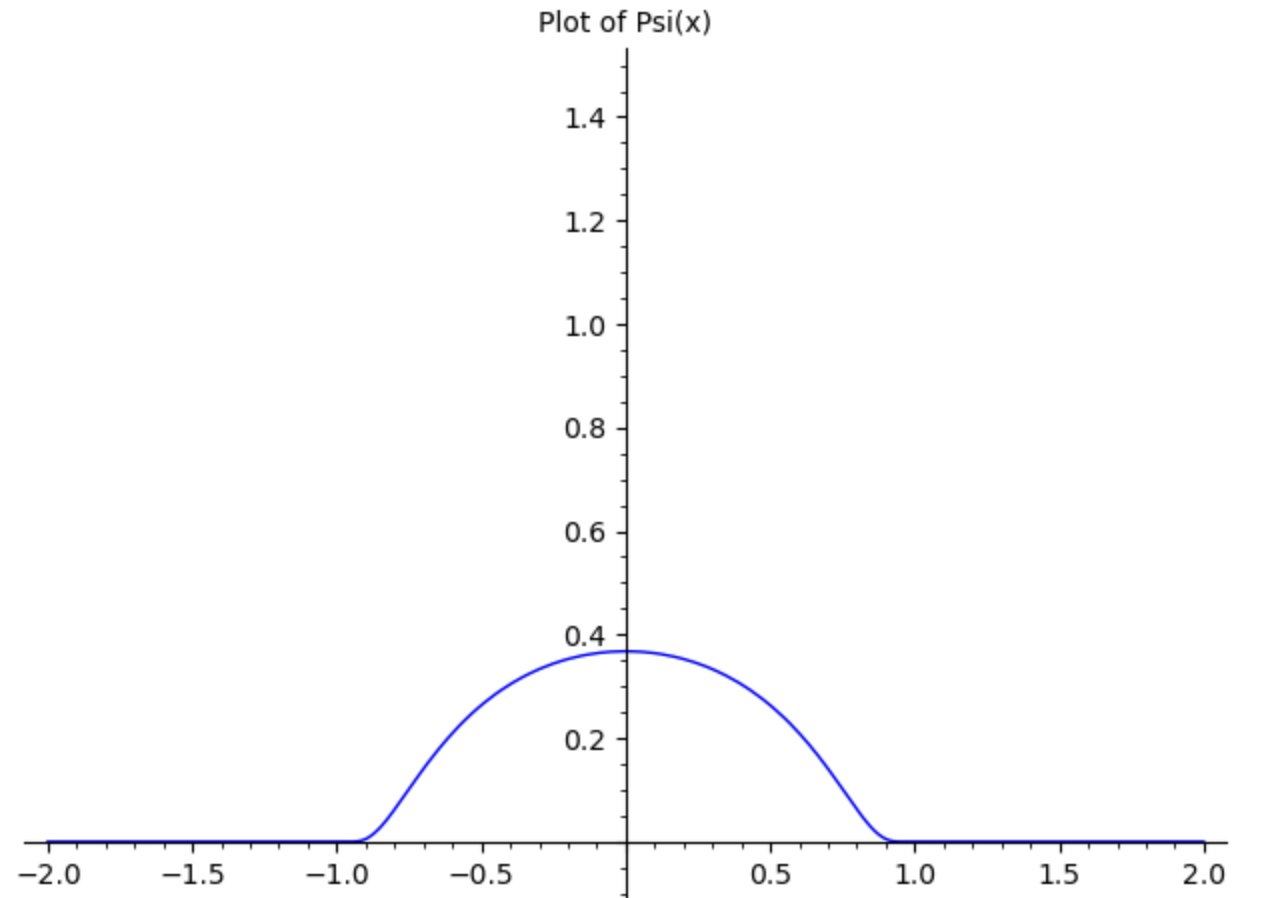
\includegraphics[height=6cm,width=16cm]{Psi_graph}
   \end{minipage}
\end{center}
Consider the smooth function $f:\R\rightarrow \R$ defined by 
\begin{align*}
f(x)\triangleq \begin{cases}
  e^{\frac{-1}{x}}& \text{ if $x>0$ }\\
  0& \text{ if $x\leq 0$ }
\end{cases}
\end{align*}
\begin{center}
   \begin{minipage}{0.9\linewidth}  
       \centering
       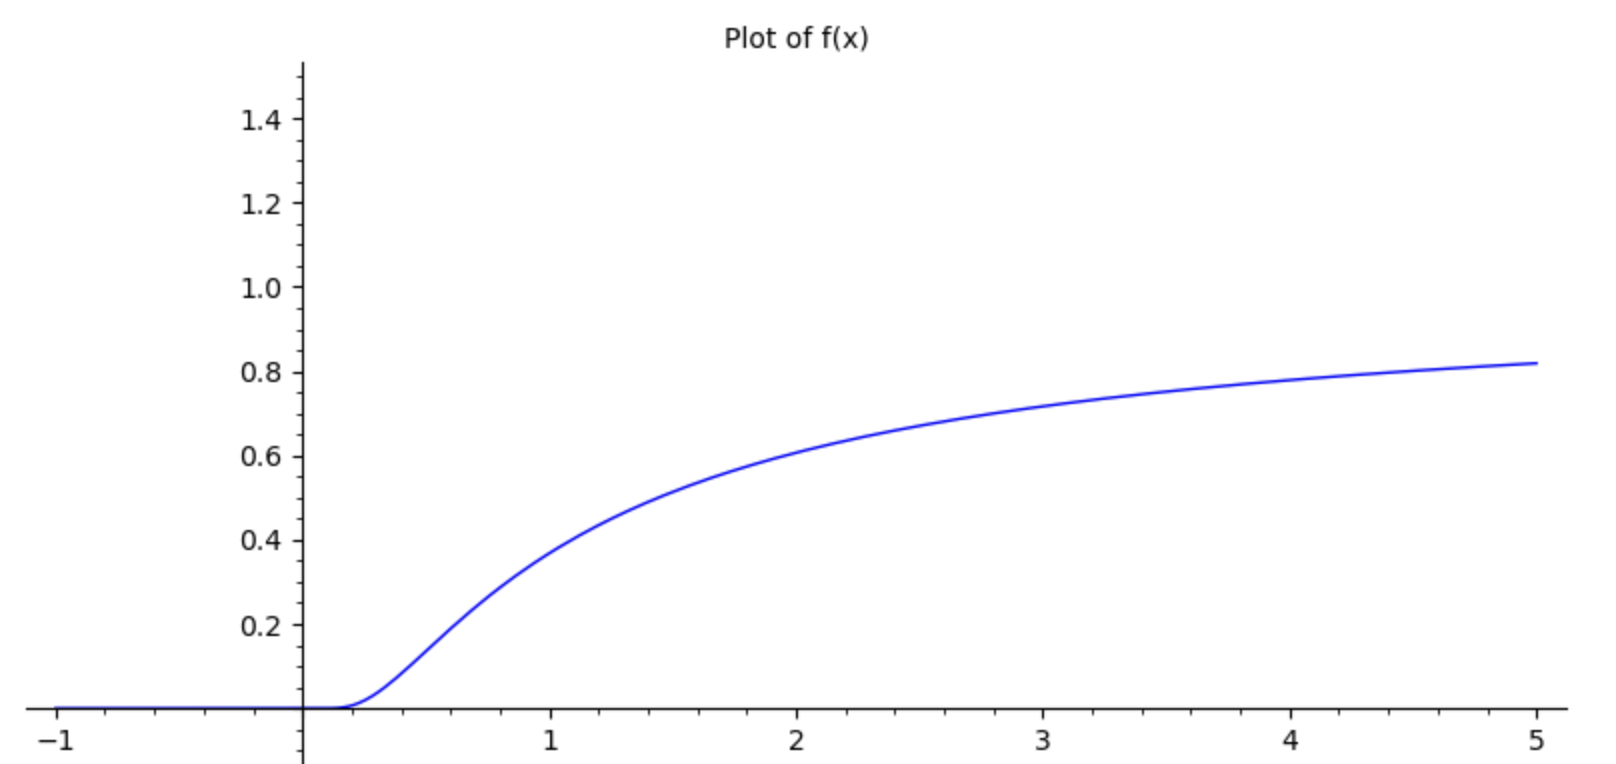
\includegraphics[height=6cm,width=16cm]{f_graph}
   \end{minipage}
\end{center}
and  $g:\R\rightarrow \R$ defined by 
\begin{align}
\label{gsm}
g(x)\triangleq \frac{f(x)}{f(x)+f(1-x)}
\end{align}
\begin{center}
   \begin{minipage}{0.9\linewidth}  
       \centering
       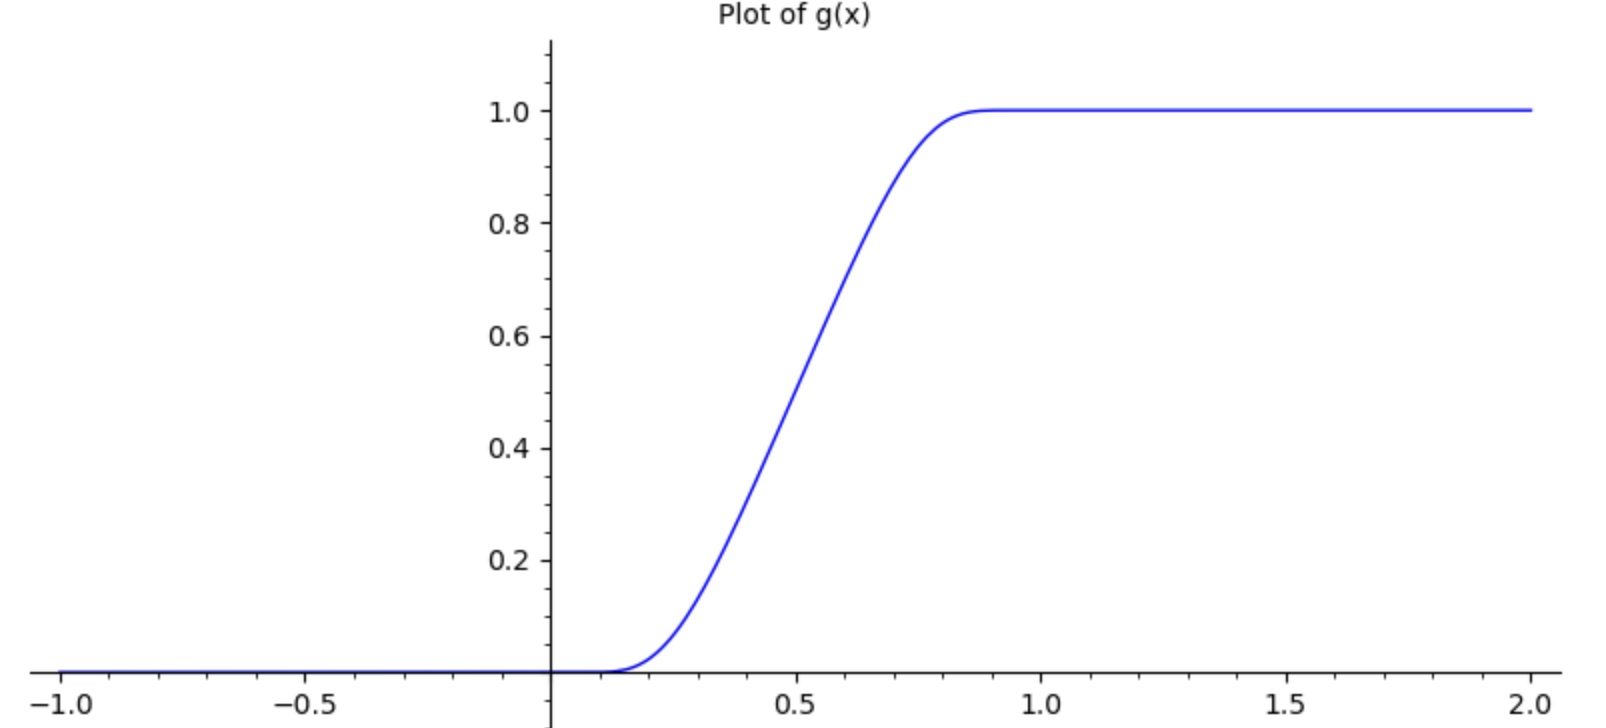
\includegraphics[height=6cm,width=16cm]{g_graph}
   \end{minipage}
\end{center}
which is a smooth increasing function such that  
\begin{align*}
g(x)=\begin{cases}
  0& \text{ if $x\leq 0$ }\\
  1& \text{ if $x\geq 1$ }
\end{cases}\text{ and }g(x)\in (0,1)\text{ if }x\in (0,1)
\end{align*}
Lastly, if we define $h:\R\rightarrow \R$ by
\begin{align*}
h(x)\triangleq g(2+x)g(2-x)
\end{align*}
\begin{center}
   \begin{minipage}{0.9\linewidth}  
       \centering
       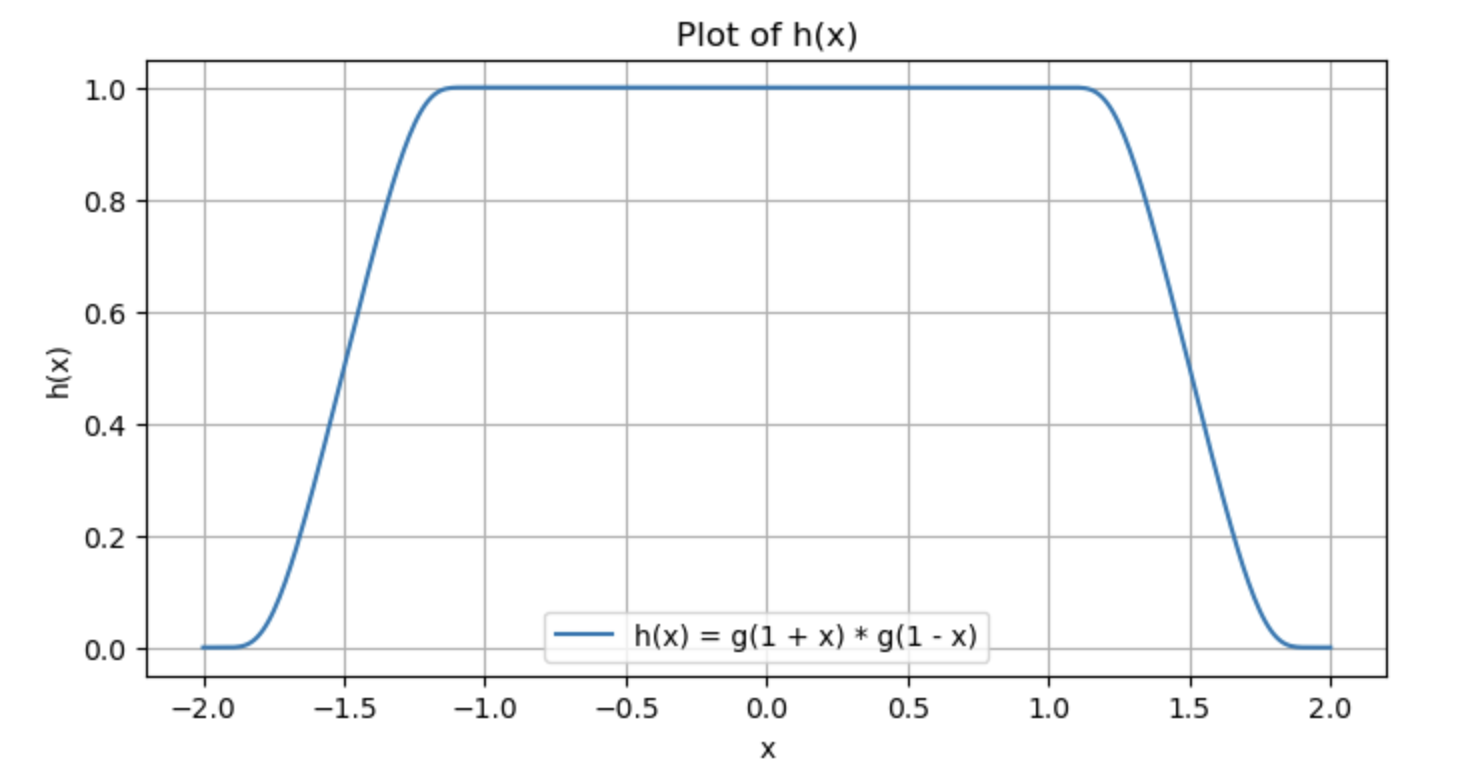
\includegraphics[height=6cm,width=16cm]{h_graph_rev}
   \end{minipage}
\end{center}
We see that $h$ is a smooth function and 
\begin{align*}
h(x)=\begin{cases}
  1& \text{ if $\abso{x}\leq 1$ }\\
  0& \text{ if $\abso{x}\geq 2$ }
\end{cases}\text{ and }h(x)\in (0,1)\text{ if } 1< \abso{x}< 2
\end{align*}
A $n$-dimensional generalization of this smooth function $h$ is  $H:\R^n\rightarrow \R$ defined by 
\begin{align*}
H(\textbf{x})\triangleq  h\Big(\frac{\abso{\textbf{x}}}{r}\Big)
\end{align*}
which is a non-negative smooth function such that 
\begin{align*}
H(\textbf{x})>0\text{ if and only if }\abso{\textbf{x}}< 2r
\end{align*}
\end{mdframed}
\begin{theorem}
\label{Smooth manifolds always admit smooth partition of unity}
\textbf{(Smooth manifolds always admit smooth partition of unity)} Given a smooth manifold $M$ and some open cover  $(U_\alpha )$ of $M$, there exists some smooth partition of unity  $(\psi_\alpha )$ subordinate to $(U_\alpha )$. 
\end{theorem}
\begin{proof}
For each $U_\alpha $ and each chart $(V,\phi)$ contained by $U_\alpha $, if we let $\mathcal{B}_{\alpha ,V}$ be the collection of the pre-images of the open balls $B_r(x)$ in $\phi (V)$ that satisfy $\exists r'>r:B_{r'}(x)\subseteq \phi (V)$, we know that $\mathcal{B}_{\alpha ,V}$ form a basis of $V$. It follows that there exists a basis $\mathcal{B}_\alpha $ for $U_\alpha $ of the form $\mathcal{B}_\alpha \triangleq \bigcup_{(V,\phi)\subseteq U_\alpha }\mathcal{B}_{\alpha ,V}$ and a basis $\mathcal{B}$ for $M$ of the form  $\mathcal{B}\triangleq \bigcup_{\alpha}\mathcal{B}_\alpha $. By \myref{Theorem}{Topological Manifold are Paracompact}, we know there exists a countable locally finite open refinement $(B_n)$ of $U_\alpha $ consisting of element of $\mathcal{B}$.\\

Now, for each $n$, there exists corresponding chart $(V,\phi)$ and $r,r'$ such that  
 \begin{align*}
   \phi (B_n)=B_r(x)\text{ and }\overline{B_r(x)}\subseteq B_{r'}(x)\subseteq \phi (V)
\end{align*}
This with some tedious effort guarantee that  
\begin{align*}
\overline{B_n}=\phi^{-1}(\overline{B_r(x)})
\end{align*}
We then can well-define a function $f_n:M\rightarrow \R$ by 
\begin{align*}
f_n \triangleq \begin{cases}
  H_n \circ \phi &\text{ on }V\\
  0&\text{ on }M\setminus \overline{B_n}
\end{cases}
\end{align*}
where $H_n:\R^n\rightarrow \R$ is a smooth function that is positive on $B_r(x)$ and zero else where. (One should at this point check that $f_n$ is well-defined)\\

Since $V$ and  $M \setminus \overline{B_n}$ are both open and $f_n$ are both smooth on them, we now see  $f_n$ is smooth on the whole  $M$. Now, since $(B_n)$ is a locally finite cover of $M$ and $f_n$ can only be positive on  $B_n$, we see that the function $f:M\rightarrow \R$ 
\begin{align*}
f(x)\triangleq \sum_{n\inn}f_n(x)\text{ is well defined }
\end{align*}
and that $f$ is positive on whole $M$  because each $f_n$ is positive on $B_n$ and $(B_n)$ cover the whole $M$. Note that $f$ is also smooth on $M$ since for each $x$, there exists an open-neighborhood around $x$ on which $f$ is just a finite sum of $f_n$. We now can define for each $n$ a smooth function  $g_n:M\rightarrow \R$ by 
\begin{align*}
g_n(x)\triangleq \frac{f_n(x)}{f(x)}
\end{align*}
Lastly, because $(B_n)$ is an open refinement of $U_\alpha $, we can associate each $n$ with an $\alpha (n)$ satisfying $B_n \subseteq U_{\alpha (n)}$. Then, because $g_n$ are non-negative and  $\sum_{n\inn}g_n\equiv 1$, we can define for each $\alpha $ a function $\psi_\alpha :M\rightarrow \R$ by 
\begin{align*}
\psi_\alpha \triangleq \sum_{n:\alpha (n)=\alpha } g_n
\end{align*}
Because $(B_n)$ is locally finite and $g_n$ is only positive on $B_n$, we see that  $\psi_\alpha $ is indeed smooth. Some tedious effort shows that $\psi_\alpha $ is indeed a partition of unity.  

\end{proof}
\begin{corollary}
\label{EoSB}
\textbf{(Existence of smooth function)} Given some  $U$ open in $M$ and some $K$ closed in $M$ and contained by  $U$, there exists a smooth function  $\psi : M\rightarrow [0,1]$ such that 
\begin{enumerate}[label=(\alph*)]
  \item $\psi \equiv 1$ on $K$. 
  \item $\operatorname{supp}\psi \subseteq U$
\end{enumerate}
\end{corollary}
\begin{corollary}
\label{EoSF}
\textbf{(Extension of Smooth Function)} Suppose $K$ is closed in $M$, and $U$ is open in  $M$ while containing  $K$. For all $f\in C^{\infty}(U)$, there exists $\tilde{f}\in C^{\infty}(M)$ such that $\tilde{f}|_K=f$ and $\operatorname{supp}\tilde{f}\subseteq U$. 
\end{corollary}
\begin{proof}
\myref{Corollary}{EoSB} give us a smooth function $\psi \in C^{\infty}(M)$ such that $\psi \equiv 1$ on $K$ and  $\operatorname{supp}\psi \subseteq U$. We simply define 
\begin{align*}
\tilde{f}(p)\triangleq \begin{cases}
  \psi(p) f (p)& \text{ if $p\in  U$ }\\
  0& \text{ if $p\not\in U$ }
\end{cases} 
\end{align*}
It is clear that $\tilde{f}|_K=f$. To see $\operatorname{supp}\tilde{f} \subseteq U$, check $\operatorname{supp}\tilde{f} \subseteq \operatorname{supp}\psi$. It is clear that $\tilde{f}$ is smooth on $U$. To see $\tilde{f}$ is smooth at all $p\not\in U$, observe that $\tilde{f}\equiv 0$ on some neighborhood around $p$. 
\end{proof}
\begin{mdframed}
Before we state the next Theorem, we shall point out that since topological manifolds are locally Euclidean, they are locally connected, and thus \customref{local-path}{the connected components of a topological manifold are identical to the path-connected components}.  
\end{mdframed}
\begin{theorem}
\textbf{(Existence of Smooth Curve)} If $p,q$ are in the same connected component of smooth manifold $M$, then there exists a smooth curve $\gamma :[0,1]\rightarrow M$ joining $p,q$. By $\gamma $ being smooth, we mean $\gamma $ is smooth on $(0,1)$. 
\end{theorem}
\begin{proof}
  We first show that \olive{there exists a piece-wise smooth curve $\alpha:[0,1]\rightarrow M$ joining $p,q$}. Let $\gamma_0:[0,1]\rightarrow M$ be a curve joining $p,q$. We know there exist a collection of chart  $(U_\alpha ,\phi_\alpha )$ covering the image of $\gamma_0$ such that $U_\alpha $ are homeomorphically mapped to an open ball in $\R^n$ by  $\phi_\alpha $. Now, because image of $\gamma _0$ is compact, we can suppose the collection $(U_j,\phi_j)_{j=1}^N$ is finite. Note that $\gamma _0^{-1}(U_j)$ form an open cover for the metric space $[0,1]$. It then follows from \customref{Lebesgue's Number Lemma}{Lebesgue's Number Lemma} that there exists $n\inn$ such that  \begin{align*}
\text{ For all $k\in \set{1,\dots ,n}$ there exists some $j_k$ such that }\gamma_0([\frac{k-1}{n},\frac{k}{n}])\subseteq U_{j_k}  
\end{align*}
Because $\phi_j(U_j)$ is an open ball in $\R^d$, we can now join  $\gamma_0 (\frac{k-1}{n}),\gamma _0 (\frac{k}{n})$ with a straight line in $\phi_{{j_k}}(U_{j_k})$. In other words, for each $k$, we define $\gamma _k:[0,1]\rightarrow M$ 
\begin{align*}
  \gamma_k (t)\triangleq \phi_{j_k}^{-1}\Big[\phi_{j_k}\Big(\gamma_0 (\frac{k-1}{n})\Big)+ t[\phi_{j_k}\Big(\gamma_0 (\frac{k}{n}) \Big) - \phi_{j_k}\Big(\gamma_0 (\frac{k-1}{n}) \Big)] \Big]
\end{align*}
and 
\begin{align*}
\alpha (t)\triangleq \gamma_k (nt-k)\text{ if }t\in [\frac{k-1}{n}, \frac{k}{n}] \odone
\end{align*}
Lastly, we construct $\gamma $ by adjusting the "speed" of $\alpha $ so that it is also smooth at each $\gamma_0 (\frac{k}{n})$ for $1\leq k\leq n-1$. For this, we use the smooth function $g:\R\rightarrow \R$ we defined earlier in \myref{Equation}{gsm} and define 
\begin{align*}
\gamma (t)\triangleq \gamma_k (g(nt-k))\text{ if }t\in [\frac{k-1}{n}, \frac{k}{n}] 
\end{align*}
To see $\gamma $ is indeed smooth, note that $[ \frac{k-1}{n}-\epsilon , \frac{k}{n}+ \epsilon ]$ is contained by  $\gamma_0^{-1}(U_{j_k})$ and the curve $\phi_{j_k}\circ \gamma : [\frac{k-1}{n}-\epsilon , \frac{k}{n}+\epsilon ]\rightarrow \R^d$ is smooth for each $n$. 
\end{proof}
\section{Tangent Space}
\begin{abstract}
In this section and from now on, $C^{\infty}(M)$ denote the space of all smooth real-valued function defined on $M$. 
\end{abstract}
\begin{mdframed}
Given a point $p$ in  $M$, we define the  \textbf{tangent space $T_pM$ of $M$ at $p$} to be the space of linear functional $D:C^{\infty}(M)\rightarrow \R$ that satisfy the product rule at $p$ 
 \begin{align*}
   D(fg)=D(f) g(p)+ f(p)D(g)\text{ for all }f,g\in C^{\infty}(M)
\end{align*}
It is clear that tangent space form a vector space when endowed with pointwise scalar multiplication and addition. Note that 
\begin{align*}
D(1)=D(1^2)=D(1)+D(1)
\end{align*}
This implies that for all $D \in T_pM$, if  $f\in C^{\infty}(M)$ is constant, then $D(f)=0$. 
\end{mdframed}
\begin{theorem}
\label{Dtprn}
\textbf{(Dimension of $T_\textbf{p}\R^n$ is $n$)} For all $\textbf{p}\inr^n$, the vector space $T_\textbf{p}\R^n$ is $n$-dimensional. 
\end{theorem}
\begin{proof}
Define a function $\phi:\R^n\to T_\textbf{p}(\R^n)$ by 
\begin{align*}
\textbf{x}\mapsto D_\textbf{x}\text{ where }D_\textbf{x}(f)= \textbf{x}\cdot \nabla f(\textbf{p})
\end{align*}
It is straightforward to check that $\phi$ is well defined and a linear transformation. It remains to prove $\phi$ is bijective. Let $D_\textbf{y}=0$, to show \vi{$\phi$ is one-to-one}, we are required to show $\textbf{y}=0$. For each $j \in \set{1,\dots, n}$, define a smooth function $g_j:\R^n\rightarrow \R$ by
\begin{align}
\label{fjxj}
g_j(\textbf{x})\triangleq \textbf{x}^j
\end{align}
We then see that for all $\textbf{y}\inr^n$
\begin{align*}
D_\textbf{y}(g_j)=\textbf{y}\cdot \textbf{e}_j= \textbf{y}^j
\end{align*}
Then if $D_\textbf{y}=0$, we must have $\textbf{y}=0$. $\vdone$ \\

We now show \blue{$\phi$ is onto}. Fix $w\in T_p(\R^n)$ and define $\textbf{v}\inr^n$ by 
\begin{align*}
\textbf{v}^j \triangleq w(g_j)
\end{align*}
where $g_j$ is defined in  \myref{Equation}{fjxj}. We claim \blue{$w=D_\textbf{v}$}. Fix $f \in C^{\infty}(\R^n)$. By \customref{Multi Taylor}{Multi Variables Taylor Theorem}, we know 
\begin{align}
  f(\textbf{x})=f(\textbf{p})&+ \sum_{i=1}^n \frac{\partial f}{\partial \textbf{x}^i}(\textbf{p})(\textbf{x}^i - \textbf{p}^i)\notag
 \\ 
 & +\sum_{i,j=1}^n (\textbf{x}^i-\textbf{p}^i)(\textbf{x}^j-\textbf{p}^j)\int_0^1 (1-t) \frac{\partial f}{\partial \textbf{x}^i \partial \textbf{x}^j}(\textbf{p}+t (\textbf{x}-\textbf{p}))dt \label{vp}
\end{align}
Now, putting both side into $w$, by product rule we can cancel \myref{term}{vp}, so
 \begin{align*}
w(f)= \sum_{i=1}^n \frac{\partial f}{\partial \textbf{x}^i}(\textbf{p})w(g_i)= \sum_{i=1}^n \frac{\partial f}{\partial \textbf{x}^i}(\textbf{p})\textbf{v}^i= D_\textbf{v}(f) \bdone
\end{align*}
\end{proof}
\begin{mdframed}
As pointed out by the proof of \myref{Theorem}{Dtprn}, for each $D_\textbf{x}\in T_\textbf{p}\R^n$, the value of $D_\textbf{x}(f)$ is determined locally at $\textbf{p}$ by $f$. The same behavior happens in the general case. 
\end{mdframed}
\begin{theorem}
\label{Tangent Vector care only about local behavior}
\textbf{(Tangent Vector care only about local behavior)} Suppose $v \in T_pM$. If $f,g \in C^{\infty}(M)$ agree on some open neighborhood around $p$, then  $v(f)=v(g)$. 
\end{theorem}
\begin{proof}
Let $h\triangleq f-g \in C^{\infty}(M)$. We know $h\equiv 0$ on some open neighborhood around $p$. This implies 
 \begin{align*}
\operatorname{supp}(h)\subseteq M \setminus \set{p}\subseteq M
\end{align*}
By \myref{Corollary}{EoSB}, there exists some smooth function $\psi : M \rightarrow [0,1]$ such that $\psi \equiv 1$ on $\operatorname{supp}(h)$ and $\operatorname{supp}(\psi)\subseteq M \setminus \set{p}$. Since $\operatorname{supp}(\psi )\subseteq M \setminus \set{p}$, we know $\psi (p)=h(p)=0$, and since $\psi \equiv 1$ on $\operatorname{supp}(h)$, we also know $\psi h=h$. This let us deduce 
\begin{align*}
v(h)=v(\psi h)=v(\psi)h(p)+\psi (p) v(h)=0  
\end{align*}



\end{proof}
\begin{mdframed}
We now define the derivative  $F_{*,p}:T_pM\rightarrow T_{F(p)}N$ of a smooth map $F:M\rightarrow N$ at $p\in  M$ between smooth manifold. 
\begin{align*}
  (F_{*,p}(w))(f)\triangleq w(f\circ F)
\end{align*}
It is straightforward to check that given another smooth manifold $R$ and smooth map  $G:N\rightarrow R$ we have
\begin{enumerate}[label=(\alph*)]
  \item $F_{*,p}(w) \in T_{F(p)}N$. 
  \item  $F_{*,p}$ is linear.  
  \item $(G\circ F)_{*,p}=G_{*,F(p)}\circ F_{*,p}:T_pM\rightarrow T_{G\circ F(p)}R$. 
  \item If $\textbf{id}:M\rightarrow M$ is the identity function on $M$, then $\textbf{id}_{*,p}$ is the identity map on $T_pM$. 
  \item If $F:M\rightarrow N$ is a diffeomorphism, then  $F_{*,p}:T_pM \rightarrow T_{F(p)}(N)$ is an isomorphism of vector space and $(F_{*,p})^{-1}=(F^{-1})_{*,F(p)}$
\end{enumerate}

\end{mdframed}
\begin{theorem}
\label{TSop}
\textbf{(Tangent Space of points in open restriction)} Given some open subset $U \subseteq M$ and inclusion map $\diota  :U\rightarrow M $, for all $p \in U$, the map $\diota _{*,p}:T_pU\rightarrow T_pM$ is a vector space isomorphism.  
\end{theorem}
\begin{proof}
  We first prove that \vi{$\diota _{*,p}$ is one-to-one}. Fix $v \in T_pU$ such that $\diota_{*,p}(v)=0$.  We are required to show \vi{$v=0$}. Fix $f\in C^{\infty}(U)$. Let $(V,\phi)$ be a chart contained in $U$ and centering $p$, and let  $\epsilon $ satisfy 
\begin{align*}
  \overline{B_\epsilon (\phi (p))}\subseteq \phi (V)  
\end{align*}
Define  $K\triangleq  \overline{\phi ^{-1}(B_\epsilon (\phi (p)))}$. By \myref{Corollary}{EoSF}, we know there exists $\tilde{f}\in C^{\infty}(M)$ such that $\tilde{f}\equiv f$ on $K$. Then because \customref{Tangent Vector care only about local behavior}{tangent vector care only about local behavior}, we can now deduce 
  \begin{align*}
  v(f)=v(\tilde{f}|_U )=v(\tilde{f}\circ \diota   )=\iota_{*,p}(v)(\tilde{f}) =0 \vdone
  \end{align*}
  We now prove $\blue{\iota_{*,p}\text{ is onto}}$. Fix $w\in T_pM$, and again  $K\triangleq \overline{\phi^{-1}(B_\epsilon (\phi (p)))}$. Define $v\in T_pU$ by 
\begin{align*}
v(f)\triangleq w(\tilde{f})
\end{align*}
where $\tilde{f}\in C^{\infty}(M)$ satisfy $\tilde{f}\equiv f$ on $K$. Because for all $g\in C^{\infty}(M)$, $g \equiv g \circ \diota  $ on $K$, we know 
\begin{align*}
\iota_{*,p}(v)(g)=v(g\circ \diota )= w(g) \bdone
\end{align*}
\end{proof}
\begin{mdframed}
Given a chart $(U,\phi)$ containing $p$, we often define $\frac{\partial }{\partial \textbf{x}^i}|_p\in T_pM$ by
\begin{align}
\label{tsbasis}
\frac{\partial }{\partial \textbf{x}^i}\Big|_p (f) \triangleq \frac{\partial (f\circ \phi^{-1})}{\partial \textbf{x}^i}(\phi (p))
\end{align}
By \myref{Theorem}{TSop}, we have the following diagram 
\[\begin{tikzcd}
	{T_pM} &&& {T_{\varphi (p)}\R^m} \\
	\\
	{T_pU} & {} && {T_{\varphi(p)}\varphi(U)}
	\arrow["{\dot{\iota}_{*,\varphi(p)}}"', leftrightarrow, from=1-4, to=3-4]
	\arrow["{\dot{\iota}_{*,p}}"', leftrightarrow, from=3-1, to=1-1]
	\arrow["{\varphi_{*,p}}", leftrightarrow, from=3-1, to=3-4]
\end{tikzcd}\]
Then since $\frac{\partial}{\partial \textbf{x}^i}|_{\phi (p)}$ form a basis for $T_p\R^m$ by the proof of  \myref{Theorem}{Dtprn}, we see $\frac{\partial }{\partial \textbf{x}^i}|_p$ form a basis for $T_pM$. Note that our notation give us the convenient 
\begin{align*}
\frac{\partial }{\partial \textbf{x}^i}\Big|_p= \sum_j \frac{\partial \tilde{\textbf{x}}^j }{\partial \textbf{x}^i} \frac{\partial  }{\partial \tilde{\textbf{x}}^j }\Big|_p
\end{align*}
when we are given another chart containing $p$.  (Verify this by some tedious effort) \\






Now, if we define for each $C^1$ curve $\gamma:(-\epsilon , \epsilon )\rightarrow M$ such that $\gamma  (0)=p$, its \textbf{velocity vector $\gamma '(0) \in T_{\gamma (0)}M$} by 
\begin{align*}
\gamma '(0)(f)\triangleq (f\circ \gamma )'(0)
\end{align*}
we see that every tangent vector $v \in T_p M$ can be identified as a velocity vector of some smooth curve 
\begin{align*}
\gamma (t)\triangleq \phi^{-1}(v^1t,\dots ,v^nt)\text{ where }v= \sum v^i \frac{\partial }{\partial \textbf{x}^i}\Big|_p
\end{align*}
Moreover, we see that smooth map $F:M\rightarrow N$ preserve velocity in the sense that 
\begin{align*}
F_{*,p}(\gamma '(0))= (F\circ \gamma )'(0)
\end{align*}
This give an expected result. 
\end{mdframed}
\begin{theorem}
\textbf{(Constant function)} If at each point $p\in  M$, the derivative $F_{*,p}$ of the smooth map $F:M\rightarrow N$ is null, then $F$ is constant on each path-connected component of $M$. 
\end{theorem}
\begin{proof}
Fix $p,q$ in the same connected component of  $M$, and let  $\gamma :[0,1]\rightarrow M$ be a smooth curve joining them and lying inside the connected component. \As{$F(p)\neq F(q)$}. Let $(V,\psi)$ be a chart centering $F(p)$ and let $B$ be a regular coordinate ball (with respect to $(V,\psi)$) centering  $F(p)$ such that $F(q)\not\in \overline{B}$, and let $f\in C^\infty (N)$ be a non-negative smooth function positive on and only on $B$. Because $F_{*,p}$ are null, we can deduce
\begin{align*}
  (f\circ F\circ \gamma )'(t)=(F\circ \gamma )'(t)(f)=0\text{ for all }t\in (0,1)
\end{align*}
It then follows that $f(F(p))=f(F(q))$. \CaC 
\end{proof}
\section{Inverse Function Theorem and Rank Theorem} 
\begin{abstract}
In this section, we prove the \customref{Inverse Function Theorem for Manifolds}{Inverse Function Theorem for Manifolds} with \customref{IFT}{Inverse Function Theorem for Euclidean Spaces} and prove  \customref{Rank Theorem for Manifolds}{Rank Theorem for Manifolds} with \customref{Inverse Function Theorem for Manifolds}{Inverse Function Theorem for Manifolds}. 
\end{abstract}
\begin{mdframed}
Given a function $F:M\rightarrow N$ differentiable at some point $p\in  M$, we define \textbf{the rank of $F$ at $p$} to be the rank of the linear map $F_{*,p}:T_pM\rightarrow T_{F(p)}N$. Let $(V,\psi)$ be a  chart containing $F(p)$ and $(U,\phi)$ be a chart containing $p$ while  $F(U)\subseteq V$. To find the rank of $F_{*,p}$, we are required to compute the matrix representation $[F_{*,p}]$ with respect to the basis $ \frac{\partial }{\partial \textbf{x}^i}|_p  $ and  $\frac{\partial }{\partial \textbf{y}^j}|_{F(p)}$. To compute $[F_{*,p}]$, we first define $\widehat{F}:\phi (U)\rightarrow \psi (V)$ and $\widehat{p}\inr^m$ by 
\begin{align*}
\widehat{F}(\textbf{x})\triangleq \psi \circ F \circ \phi ^{-1}(\textbf{x})\text{ and }\widehat{p}\triangleq \phi (p)
\end{align*}
Immediately, we see that 
\begin{align}
\label{cri}
F= \psi^{-1}\circ \widehat{F}\circ \phi 
\end{align}
This immediate result \myref{Equation}{cri} is in fact very critical, since as shall show, it is easy to compute $[\widehat{F}_{*,\widehat{p}}]$ with respect to the basis $\frac{\partial }{\partial \widehat{\textbf{x}}^i}|_{\widehat{p}}$ and $\frac{\partial }{\partial \widehat{\textbf{y}}^j}|_{\widehat{F}(\widehat{p})}$, and we by definition also have the relationship 
\begin{align}
\label{rel}
  \phi_{*,p}\Big( \frac{\partial }{\partial \textbf{x}^i}\Big|_p \Big)= \frac{\partial }{\partial \widehat{\textbf{x}}^i}\Big|_{\widehat{p}}\text{ and } (\psi^{-1})_{*,\widehat{F}(\widehat{p})} \Big( \frac{\partial }{\partial \widehat{\textbf{y}}^j}\Big|_{\widehat{F}(\widehat{p})} \Big)  = \frac{\partial }{\partial \textbf{y}^j} \Big|_{F(p)}
\end{align}
Fix smooth $f\in C^{\infty}(\R^n)$. By applying  \customref{CR}{ordinary chain rule} on $f\circ \widehat{F}$ and observing \customref{DiJ}{matrix representation of $df$ and $d \widehat{F}$}, we can compute $[\widehat{F}_{*,\widehat{p}}]$ with respect to $\frac{\partial }{\partial \widehat{\textbf{x}}^i}|_{\widehat{p}}$ and $\frac{\partial }{\partial \widehat{\textbf{y}}^j}|_{\widehat{F}(\widehat{p})}$ 
\begin{align*}
\widehat{F}_{*,\widehat{p}} \Big( \frac{\partial }{\partial \widehat{\textbf{x}}^i} \Big|_{\widehat{p}} \Big)(f)= \frac{\partial  (f\circ \widehat{F})}{\partial \widehat{\textbf{x}}^i}(\widehat{p})&= \sum_j \frac{\partial f}{\partial \widehat{\textbf{y}}^j} (\widehat{F}(\widehat{p})) \frac{\partial \widehat{F}^j}{\partial \widehat{\textbf{x}}^i}(\widehat{p}) \\
 &=\sum_j \frac{\partial \widehat{F}^j}{\partial \widehat{\textbf{x}}^i}(\widehat{p}) \Big[\frac{\partial }{\partial \widehat{\textbf{y}}^j}\Big|_{\widehat{F}(\widehat{p})}(f)\Big]
\end{align*}
This in general means that 
\begin{align*}
\widehat{F}_{*,p}\Big( \frac{\partial }{\partial \widehat{\textbf{x}}^i}\Big|_{\widehat{p}} \Big)= \sum_j \frac{\partial \widehat{F}^j}{\partial \widehat{\textbf{x}}^i}(\widehat{p}) \frac{\partial }{\partial \widehat{\textbf{y}}^j}\Big|_{\widehat{F}(\widehat{p})}
\end{align*}
Then with the relationship in \myref{Equation}{rel} and \myref{Equation}{cri}, we finally have 
\begin{align*}
F_{*,p}\Big( \frac{\partial }{\partial \textbf{x}^i}\Big|_p \Big) &= (\psi^{-1})_{*,\widehat{F}(\widehat{p})}\circ \widehat{F}_{*,\widehat{p}} \circ \phi_{*,p} \Big( \frac{\partial }{\partial \textbf{x}^i}\Big|_p \Big) \\
&=(\psi^{-1})_{*,\widehat{F}(\widehat{p})} \Big( \sum_j \frac{\partial \widehat{F}^j}{\partial \widehat{\textbf{x}}^i}(\widehat{p}) \frac{\partial }{\partial \widehat{\textbf{y}}^j}\Big|_{\widehat{F}(\widehat{p})}  \Big) \\
&=\sum_j \frac{\partial \widehat{F}^j}{\partial \widehat{\textbf{x}}^i}(\widehat{p}) (\psi^{-1})_{*,\widehat{F}(\widehat{p})} \Big( \frac{\partial }{\partial \widehat{\textbf{y}}^j} \Big|_{\widehat{F}(\widehat{p})} \Big) \\
&=\sum_j \frac{\partial \widehat{F}^j}{\partial \widehat{\textbf{x}}^i}(\widehat{p}) \frac{\partial }{\partial \textbf{y}^j}\Big|_{F(p)} 
\end{align*}
which means 
\begin{align*}
[F_{*,p}]= [d\widehat{F}_{\widehat{p}}]
\end{align*}
With this in mind and noting that in the space of  $n\times m$ real matrix, the set of real matrices of full rank is open, we see that if $F$ is smooth and $F_{*,p}$ is full rank, then there exists an open neighborhood $U$ around $p$ for which  $F_{*,q}$ is full rank if $q\in U$.  \\

Now, given a function $F:M\rightarrow N$, we say $F$ is \textbf{locally a smooth diffeomorphism at $p\in M$} if there exists some open-neighborhood $U$ around $p$ such that $F(U)$ is open in $N$ and $F|_U:U\rightarrow F(U)$ is a smooth diffeomorphism between $U$ and $F(U)$, and we say $F$ is a \textbf{local  smooth diffeomorphism} if $F$ is locally a smooth diffeomorphism at $p$ for all $p\in  M$. 
\end{mdframed}
\begin{theorem}
\label{Inverse Function Theorem for Manifolds}
\textbf{(Inverse Function Theorem for Manifolds)} Suppose $M$ and $N$ are smooth manifold, and  $F:M\rightarrow N$ is some smooth map. If for some $p\in  M$, $F_{*,p}$ is invertible, then $F$ is locally a smooth diffeomorphism at $p$. 
\end{theorem}
\begin{proof}
Let  $(V,\psi)$ be a chart centering $F(p)$ and $(U,\phi)$ be a chart centering $p$ such that  $F(U)\subseteq V$. If we define $\widehat{F}:\phi (U)\rightarrow \psi (V)$ by 
\begin{align*}
\widehat{F}\triangleq \psi \circ F\circ \phi^{-1}
\end{align*}
we see that there exists some open set $\widehat{U}\subseteq \phi (U)$ containing  $\phi (p)$ such that $dF_\textbf{x}$ is invertible for all $\textbf{x}\in \widehat{U}$. Because $\widehat{F}$ is smooth, we then can apply \customref{IFT}{Ordinary Inverse Function Theorem} to have some $B_{\delta}(\textbf{0})\subseteq \widehat{U}$ such that $\widehat{F}|_{B_\delta(\textbf{0})}$ is a smooth diffeomorphism. It then follows that $F$ is a smooth diffeomorphism on  $\phi (B_\delta (\textbf{0}))$
\end{proof}
\begin{mdframed}
We say $F$ is a \textbf{smooth immersion} if $F$ is smooth and on each $p\in  M$ the differential $F_{*,p}$ is injective, and we say $F$ is a \textbf{smooth submersion} if $F$ is smooth and on each $p\in  M$ if $F$ is surjective. With \customref{Inverse Function Theorem for Manifolds}{Inverse Function Theorem for Manifolds}  in mind, we see that given smooth $F:M\rightarrow N$ 
\begin{align*}
F\text{ is a local diffeomorphism }\iff F\text{ are both immersion and submersion }
\end{align*}
\end{mdframed}
\begin{theorem}
\label{Rank Theorem for Manifolds}
\textbf{(Constant Rank Theorem for manifolds)} Given a smooth map $F:M\rightarrow N$ with constant rank $r$, for each  $p\in  M$, there exists some chart $(V,\psi)$  centering $F(p)$ and $(U,\phi)$ centering $p$ such that  $F(U)\subseteq V$ and $F$ has the coordinate representation of the form 
\begin{align*}
\widehat{F}(\textbf{x}^1,\dots ,\textbf{x}^r,\textbf{x}^{r+1},\dots ,\textbf{x}^m)=(\textbf{x}^1, \dots ,\textbf{x}^r, 0,\dots ,0)
\end{align*}
\end{theorem}
\begin{proof}
Because the Theorem is local, we may write  $F:U\subseteq \R^m\rightarrow V\subseteq \R^n$ by 
\begin{align*}
F(\textbf{x},\textbf{y})\triangleq (Q(\textbf{x},\textbf{y}),R(\textbf{x},\textbf{y}))
\end{align*}
where $Q:U\rightarrow \R^r,R:U\rightarrow \R^{n-r}$ maps $(\textbf{0},\textbf{0})$ to $\textbf{0}$. Since $F$ is of rank  $r$, we may assume   
\begin{align*}
\text{ The matrices }\begin{bmatrix}
  \frac{\partial Q^1}{\partial \textbf{x}^1}(\textbf{v})& \cdots & \frac{\partial Q^1}{\partial \textbf{x}^r}(\textbf{v}) \\
  \vdots & \ddots & \vdots \\
  \frac{\partial Q^r}{\partial \textbf{x}^1}(\textbf{v})& \cdots & \frac{\partial Q^r}{\partial  \textbf{x}^r}(\textbf{v})
\end{bmatrix}\text{ are invertible for all }\textbf{v}\in U
\end{align*}
Then if we define $\phi:U\rightarrow \R^m$ by 
\begin{align*}
\phi (\textbf{x},\textbf{y})\triangleq (Q(\textbf{x},\textbf{y}),\textbf{y})
\end{align*}
we see that 
\begin{align*}
[d\phi_\textbf{v}]= \begin{bmatrix}
  \frac{\partial Q^1}{\partial \textbf{x}^1}(\textbf{v}) & \cdots & \frac{\partial Q^1}{\partial \textbf{x}^r}(\textbf{v}) & \frac{\partial Q^1}{\partial \textbf{y}^1} (\textbf{v}) & \cdots & \frac{\partial Q^1}{\partial \textbf{y}^{m-r}}(\textbf{v}) \\
  \vdots & \ddots & \vdots & \vdots & \ddots & \vdots \\
  \frac{\partial Q^r}{\partial \textbf{x}^1}(\textbf{v}) & \cdots & \frac{\partial Q^r}{\partial  \textbf{x}^r}(\textbf{v}) & \frac{\partial Q^r}{\partial \textbf{y}^1} (\textbf{v}) & \cdots & \frac{\partial Q^r}{\partial \textbf{y}^{m-r}}(\textbf{v}) \\
  0 & \cdots & 0 & 1 & \cdots & 0\\
  \vdots & \ddots & \vdots & \vdots & \ddots & \vdots \\
  0 & \cdots & 0 & 0 &\cdots & 1 
\end{bmatrix}\text{ is invertible for all }\textbf{v}\in U
\end{align*}
It then follows from \customref{IFT}{Ordinary Inverse Function Theorem} such that there exists $U_0\subseteq U$ containing $(\textbf{0},\textbf{0})$ such that $\phi$ maps $U_0$ smooth-diffeomorphically to some open cube $\widehat{U_0}\subseteq \R^m$. \\

 It is clear for all $(\textbf{x},\textbf{y})\in \widehat{U_0}$, we have  
\begin{align*}
  (\phi|_{U_0})^{-1}(\textbf{x},\textbf{y})= (A(\textbf{x},\textbf{y}),\textbf{y})
\end{align*}
 where $A$ is some function that maps $\widehat{U_0}$ into $\R^r$. Now by definition of $\phi$, we can compute 
\begin{align*}
  (\textbf{x},\textbf{y})=\phi (A(\textbf{x},\textbf{y}),\textbf{y})= (Q(A(\textbf{x},\textbf{y}),\textbf{y}),\textbf{y})
\end{align*}
for all $(\textbf{x},\textbf{y})\in \widehat{U_0}$. This then let us compute
\begin{align*}
 Q(A(\textbf{x},\textbf{y}),\textbf{y})=\textbf{x} 
\end{align*}
for all $(\textbf{x},\textbf{y})\in \widehat{U_0}$, which implies  
\begin{align*}
F\circ \phi^{-1}(\textbf{x},\textbf{y})=F (A(\textbf{x},\textbf{y}),\textbf{y})= (\textbf{x},\tilde{R}(\textbf{x},\textbf{y}))
\end{align*}
for all $(\textbf{x},\textbf{y})\in \widehat{U_0}$ where $\tilde{R}(\textbf{x},\textbf{y})\triangleq R(A(\textbf{x},\textbf{y}),\textbf{y})$ maps $\widehat{U_0}\subseteq \R^m\text{ into }\R^{n-r}$. Now, because $\phi^{-1}:\widehat{U_0}\rightarrow U_0 \subseteq \R^m$ is full rank and $F$ is of rank  $r\leq m$, we see $F\circ \phi^{-1}:\widehat{U_0}\rightarrow \R^n$ if also of rank $r$. Then from observing that the differential of  $F\circ \phi ^{-1}$ is of the form 
\begin{align*}
[d(F\circ \phi^{-1})_{\textbf{v}}]=\begin{bmatrix} 
  1 & \cdots & 0 & 0 & \cdots & 0 \\
  \vdots & \ddots & \vdots & \vdots & \ddots & \vdots \\
  0 & \cdots & 1 & 0 & \cdots & 0  \\
  \frac{\partial \tilde{R}^1 }{\partial \textbf{x}^1}(\textbf{v}) & \cdots & \frac{\partial \tilde{R}^1 }{\partial  \textbf{x}^r}(\textbf{v}) & \frac{\partial \tilde{R}^1 }{\partial  \textbf{y}^1}(\textbf{v}) & \cdots &\frac{\partial \tilde{R}^1 }{\partial  \textbf{y}^{m-r}}(\textbf{v}) \\
  \vdots & \ddots & \vdots & \vdots & \ddots & \vdots \\
  \frac{\partial \tilde{R}^{n-r} }{\partial \textbf{x}^1}(\textbf{v}) & \cdots & \frac{\partial \tilde{R}^{n-r} }{\partial  \textbf{x}^r}(\textbf{v}) & \frac{\partial \tilde{R}^{n-r} }{\partial  \textbf{y}^1}(\textbf{v}) & \cdots & \frac{\partial \tilde{R}^{n-r} }{\partial  \textbf{y}^{m-r}}(\textbf{v}) \\
 \end{bmatrix}
\end{align*}
We can deduce 
\begin{align*}
\frac{\partial \tilde{R}^j }{\partial \textbf{y}^i}(\textbf{v})=0\text{ for all }\textbf{v}\in \widehat{U_0}\text{ and }i \in \set{1,\dots ,m-r},j \in \set{1,\dots ,n-r}
\end{align*}
This then let us write (by \customref{MVT}{MVT}) 
\begin{align}
\label{Foc}
F\circ \phi^{-1}(\textbf{x},\textbf{y})=(\textbf{x},S(\textbf{x}))
\end{align}
 for all $(\textbf{x},\textbf{y})\in \widehat{U_0}$ where $S(\textbf{x})\triangleq R(\textbf{x},\textbf{0})$. Lastly, we define $V_0\subseteq V$ by 
\begin{align*}
V_0 \triangleq \set{(\textbf{z},\textbf{w})\in V: (\textbf{z},\textbf{0})\in \widehat{U_0}} 
\end{align*}
Since $(\textbf{z},\textbf{w})\mapsto  (\textbf{z},\textbf{0})$ is a continuous map from $\R^n$ to  $\R^m$ and  $\set{(\textbf{x},\textbf{0})\inr^m:\textbf{x}\inr^r}$ is open, we see that $V_0$ is also open, which clearly contain  $(\textbf{0},\textbf{0})$.\\

Recall that $\widehat{U_0}$ is an open cube in $\R^m$; Thus from \myref{Equation}{Foc}, we can deduce
 \begin{align*}
F\circ \phi^{-1}(\widehat{U_0} ) \subseteq V_0
\end{align*}
and if we define $\psi:V_0\rightarrow \R^n$ by 
\begin{align*}
\psi (\textbf{z},\textbf{w})\triangleq (\textbf{z},\textbf{w}-S(\textbf{z}))
\end{align*}
we see $\psi$ has an explicit inverse
\begin{align*}
\psi^{-1}(\textbf{s},\textbf{t})= (\textbf{s},\textbf{t}+ S(\textbf{s}))
\end{align*}
We have established that $(V_0,\psi)$ is a smooth chart, and for all $(\textbf{x},\textbf{y})\in \widehat{U_0}$
\begin{align*}
\psi \circ F \circ \phi^{-1} (\textbf{x},\textbf{y})= (\textbf{x},\textbf{0})
\end{align*}
\end{proof}
\section{Submanifold}
\begin{abstract}
This section discuss submanifolds. Note that in this section, smooth manifold $S,M,N$ always have the dimension $s,m,n$. 
\end{abstract}
\begin{mdframed}
 By an \textbf{immersed smooth submanifold} $S$ of smooth manifold $M$, we mean a subset  $S$, endowed with a topology and a smooth structure such that the inclusion map  $\diota : S\rightarrow M$ is a smooth immersion. If we say the immersed smooth submanifold $S$ is an \textbf{embedded smooth submanifold}, we mean that the inclusion map $\diota : S \rightarrow M $ is moreover a \textbf{smooth embedding}, i.e., not only does $\diota $ have to be a smooth immersion, but $\diota  $ also have to be a topological embedding. It is clear by definition that if $S$ is an embedded smooth manifold, then the topology on $S$ must be the subspace topology.\\

  Given a subset $S$ of some smooth manifold  $M$, there exists a nice sufficient condition called  \textbf{local $k$-slice condition} for $S$ so that  $S$ can have a smooth structure that make $S$ an embedded submanifold of  $M$. We say $S$ satisfy the local $k$-slice condition if there exists a smooth atlas consisting of \textbf{$k$-slice charts $(U,\phi)$ with respect to $S$}, i.e., charts for $M$ such that  
\begin{align*}
\phi (U \cap S)= \phi (U)\cap (\R^k \times \set{\textbf{0}})
\end{align*}
\end{mdframed}
\begin{theorem}
\textbf{(Local $k$-slice condition for embedded submanifolds)} If  $S$ satisfy the local  $k$-slice condition, then $S$ have a smooth structure such that $S$ is a smooth embedded submanifold. 
\end{theorem}
\begin{proof}
Give $S$ the subspace topology. For each $k$-slice chart  $(U,\phi)$, we can define a chart $(U\cap S,\pi \circ \phi)$ for $S$ where  $\pi:\R^m \rightarrow \R^k$ is the projection defined by 
\begin{align*}
\pi (\textbf{x}^1,\dots ,\textbf{x}^m)\triangleq (\textbf{x}^1,\dots ,\textbf{x}^k)
\end{align*}
Some tedious effort shows that $(U\cap S,\pi \circ \phi )$ is indeed a chart. Because $S$ is given the subspace topology, clearly the inclusion map  $\diota $ is a topological embedding. To see that $\diota$ is also a smooth immersion, observe that for each adapted chart $(U\cap S,\pi \circ \phi)$, we have
\begin{align*}
\diota (U \cap S)\subseteq U 
\end{align*}
and for all $(\textbf{x}^1,\dots ,\textbf{x}^k)\in \pi \circ  \phi (U \cap S)$ 
\begin{align*}
\phi \circ \diota \circ (\pi \circ \phi)^{-1}(\textbf{x}^1,\dots ,\textbf{x}^k)=  (\textbf{x}^1,\dots ,\textbf{x}^k, 0,\dots ,0)
\end{align*}
This shows that $\diota $ is indeed also a smooth immersion.  
\end{proof}
\begin{mdframed}
As the next Theorem shows, the term smooth embedding is in fact very strong. 
\end{mdframed}
\begin{theorem}
\label{Ios}
\textbf{(Image of smooth embedding is always a smooth embedded submanifold)} If $F:M\rightarrow N$ is a smooth embedding, then the topology and smooth structure of $F(M)$ inherited from $M$ makes  $F(M)$ a smooth embedded manifold of $N$.  
\end{theorem}
\begin{proof}
Because $F$ is by definition a topological embedding, it is clear that $F(M)$ is endowed with the subspace topology. Fix $p \in F(M)$. Because $F$ is a smooth immersion, by  \customref{Rank Theorem for Manifolds}{Constant Rank Theorem for manifolds}, we know there exists some chart  $(U,\phi)$ for $M$ centering $F^{-1}(p)$ and some chart $(V,\psi)$ for $N$ centering  $p$ such that  $F(U)\subseteq V$ and 
\begin{align*}
\widehat{F}(\textbf{x}^1,\dots ,\textbf{x}^m)=(\textbf{x}^1,\dots ,\textbf{x}^m ,0,\dots ,0)
\end{align*}
Because $F(U)$ is open in $F(M)$, we know there exists open $V'\subseteq N$ such that 
\begin{align*}
F(U)=V' \cap F(M)
\end{align*}
We now can check that $(V\cap V', \psi|_{V\cap V'})$ is a slice chart centering $p$. 
\end{proof}
\begin{mdframed}
Note that in \myref{Theorem}{Ios}, we have in fact proved that smooth embedded submanifold always satisfy local $k$-slice condition. 


\end{mdframed}
\begin{theorem}
\label{Constant Rank Level Set Theorem}
\textbf{(Constant Rank Level Set Theorem)} If smooth $F:M\rightarrow N$ is of constant rank $k$, then level sets  $F^{-1}(q)$ for each $q\in N$ is an embedded submanifold of $M$ of  dimension $m-k$. 
\end{theorem}
\begin{proof}
Fix $p \in F^{-1}(q)$. By \customref{Rank Theorem for Manifolds}{Constant Rank Theorem for Manifold}, there exist some chart $(U,\phi),(V,\psi)$  centering $p,q$ such that  $F(U)\subseteq V$ and for all $(\textbf{x}^1,\dots ,\textbf{x}^m)\in \phi (U)$
\begin{align}
\label{psf}
\psi \circ F \circ \phi^{-1}(\textbf{x}^1,\dots ,\textbf{x}^m)= (\textbf{x}^1,\dots ,\textbf{x}^k,0,\dots ,0)
\end{align}
We now prove that $(U,\phi)$ is a  $m-k$-slice chart with respect to $F^{-1}(q)$. Let $s \in F^{-1}(q)\cap U$. Compute 
\begin{align*}
\psi \circ F(s)=\psi (q)=\textbf{0}
\end{align*}
Then since
\begin{align*}
\textbf{0}=\psi \circ F (s)= \psi \circ F \circ  \phi ^{-1}(\phi (s))
\end{align*}
from \myref{Equation}{psf}, we can deduce the first $k$ component of  $\phi (s)$ must be $0$. We have proved 
 \begin{align}
  \label{ucp}
   \phi (U\cap F^{-1}(q))\subseteq \phi (U)\cap (\set{\textbf{0}}\times \R^{m-k})
\end{align}
On the other hand, if $s \in U$ and $\phi (s)\in \set{\textbf{0}}\times \R^{m-k}$, then if we write 
\begin{align*}
\phi (s)=(0,\dots ,0,\textbf{x}^{k+1},\dots ,\textbf{x}^m)
\end{align*}
we have from \myref{Equation}{psf} that 
\begin{align*}
\psi \circ F (s)=\textbf{0}
\end{align*}
which give us $F(s)=q$. It then follows that $\phi (s)\in \phi (U \cap F^{-1}(q))$, proving the converse of \myref{Equation}{ucp}. 
\end{proof}
\begin{mdframed}
  We now generalize \customref{Constant Rank Level Set Theorem}{Constant Rank Level Set Theorem} to general smooth map. Given some smooth map $F:M\rightarrow N$, we say $p \in M$ is a \textbf{regular point} if $F_{*,p}$ is surjective; otherwise, we say $p$ is a  \textbf{critical point}. Given  $q \in N$, if $F^{-1}(q)$ contain only regular point, then we say $q$ is a \textbf{regular value}; otherwise, we say $q \in N$ is a \textbf{critical value}. If $q \in N$ is some regular value, we say $F^{-1}(q)$ is a \textbf{regular level set}. 
\end{mdframed}
\begin{theorem}
\label{Regular Level Set Theorem}
\textbf{(Regular Level Set Theorem)} Given smooth map $F:M\rightarrow N$, if $q\in N$ is some regular point, the regular level set $F^{-1}(q)$ is a smooth embedded submanifold of $M$ with dimension  $m-n$. 
\end{theorem}
\begin{proof}
  Let $U\subseteq M$  be the collection of regular points.  Because the set of full rank matrix is open in  $M_{n\times m}(\R)$ and $F$ is smooth, we can deduce  $U$ is open. Therefore, from \customref{Constant Rank Level Set Theorem}{Constant Rank Level Set Theorem}, we can deduce that $F^{-1}(q)$ is an embedded smooth submanifold of $U$. Some tedious effort and the fact \customref{TSop}{that $\diota_{*,p}:T_pU \rightarrow T_pM $ is a vector space isomorphism} now shows that $F^{-1}(q)$ is also an embedded smooth manifold of $M$. 
\end{proof}
\begin{mdframed}
Note that in \customref{Regular Level Set Theorem}{Regular Level Set Theorem}, because $F$ in priori has a regular point, we have the assumption that  $m\geq n$. As a corollary of the \customref{Regular Level Set Theorem}{Regular Level Set Theorem}, we see that  $S^n$ is regular level set  $f^{-1}(1)$ of the smooth map $f:\R^{n+1}\rightarrow \R$ defined by 
\begin{align*}
f(\textbf{x})\triangleq \abso{\textbf{x}}^2
\end{align*}
It then follows that $S^n$ is an embedded smooth submanifold of  $\R^{n+1}$.\\

Although \customref{Regular Level Set Theorem}{regular level set Theorem} shows that regular level set is always a smooth embedded submanifold, one should note that that critical level sets can sometimes also be an embedded submanifold. Consider smooth $f:\R^2 \rightarrow \R$ defined by 
\begin{align*}
f(x,y)=y^2
\end{align*}
The level set $f^{-1}(0)$ is critical everywhere but still an embedded submanifold.\\

We now go back to consider immersion. As it turned out, immersed submanifold can also be treated as the image of some injective smooth immersion. 
\end{mdframed}
\begin{theorem}
\label{Iosi}
\textbf{(Image of smooth immersion is always a smooth immersed submanifold)} Given some injective smooth immersion $F:M\rightarrow N$, the image $F(M)$ can be endowed with a topology and a smooth structure such that $F(M)$ is a smooth immersed submanifold of $N$. 
\end{theorem}
\begin{proof}
Because $F$ is injective,  we can simply give $F(M)$ the topology of $M$. For all charts $(U,\phi)$ for $M$, we can induce a chart $(F(U),\phi \circ F^{-1})$ for $F(M)$. It is clear that this indeed give a smooth structure. To see $F(M)$ is now an immersed smooth submanifold, observe that $F^{-1}:F(M)\rightarrow M$ is a smooth diffeomorphism and the inclusion map $\diota:F(M)\rightarrow N $ is the just composition of the smooth immersion  $F$ and $F^{-1}$. 
\end{proof}
\begin{mdframed}
Although there exists similarity between immersion and embedding, the latter is still strictly powerful. Consider the curve $\beta :(- \pi ,\pi)\rightarrow \R^2 $ 
\begin{align*}
\beta  (t)\triangleq (\sin 2t, \sin t)
\end{align*}
This is a smooth injective immersion, yet not a smooth embedding, since image of $\beta $ is clearly compact but $(-\pi, \pi)$ isn't shows that $\beta ^{-1}$ is not continuous. In other words, image of  $\beta $ is a smooth immersed submanifold of $\R^2$ by \myref{Theorem}{Iosi} but not a smooth embedded submanifold of $\R^2$.\\

We now shows that immersion is in fact at every point locally an embedding.  
\end{mdframed}
\begin{theorem}
\label{Local Embedding Theorem}
\textbf{(Local Embedding Theorem)} Given smooth map $F:M\rightarrow N$, $F$ is a smooth immersion if and only if for all  $p \in M$, there exists neighborhood $U$ of  $p$ in  $M$ such that  $F|_U$ is a smooth embedding. 
\end{theorem}
\begin{proof}
The if part is clear. Suppose $F$ is a smooth immersion. By \customref{Rank Theorem for Manifolds}{constant rank theorem}, there exist some charts $(U,\phi),(V,\psi)$ centering $p,F(p)$ such that $F(U)\subseteq V$ and  
\begin{align*}
\psi \circ F \circ \phi^{-1}(\textbf{x}^1, \dots ,\textbf{x}^m)=(\textbf{x}^1,\dots ,\textbf{x}^m,0,\dots ,0)
\end{align*}
It then follows that $F$ is injective on  $U$. To see that  $U$ and  $F(U)$ has the same topology, just observe that we have the following diagram
\[\begin{tikzcd}
    U &&&& {F(U)} \\
    \\
    {\varphi(U)} && {} && {\psi \circ F(U)}
    \arrow[leftrightarrow, from=1-1, to=3-1]
    \arrow[leftrightarrow, from=1-5, to=3-5]
    \arrow["{\text{obvious homeomorphism }}"', leftrightarrow, from=3-1, to=3-5]
\end{tikzcd}\]
\end{proof}
\begin{mdframed}
With \customref{Local Embedding Theorem}{local embedding Theorem}, we now see that for each $p$ in some smooth  immersed submanifold $S$ of  $M$, there exists some neighborhood  $U$ in $S$ of $p$ such that  $\diota |_U:U\rightarrow M$ is a smooth embedding; thus $U$ an embedded smooth submanifold of $M$.\\

It is easy to see that if $S$ is an immersed smooth submanifold of  $M$ and  $F:M\rightarrow N$ is a smooth map, then the restriction $F|_S$ is also a smooth map. However, it require  the fact that immersed smooth submanifold is locally an embedded submanifold to see that when we restrict the codomain of $F$, the smooth map  $F$ is still smooth.  
\end{mdframed}
\begin{theorem}
\textbf{(Smooth map is still smooth after restriction of codomain)} Given a smooth map $F:M\rightarrow N$ and an immersed smooth submanifold $S$ of $N$ such that $F(M)\subseteq S$, if $F:M\rightarrow S$ is continuous, then $F:M\rightarrow S$ is still smooth.
\end{theorem}
\begin{proof}
Fix $p \in M$ and let $q\triangleq F(p)$. We know there exists some neighborhood $U$ of $q$ in  $S$ such that  $U$ is an embedded smooth submanifold of  $N$. Then there exists some  $s$-slice chart $(V,\phi)$ for $N$ centering $q$, which give a chart $(U\cap V,\pi \circ  \phi)$ for $U$ centering $q$. Because $F:M\rightarrow N$ is a smooth map, there exists some chart $(W,\psi)$ for $M$ centering  $p$ such that  $F(W)\subseteq V$ and 
\begin{align*}
\phi \circ F \circ \psi^{-1}:\psi (W)\rightarrow \R^n\text{ is smooth }
\end{align*}
Because $F:M\rightarrow S$ is continuous and $U\cap V$ is open in $U$ which is open in  $S$, we know there exists some open set $W_0 \subseteq W$ centering $p$ such that 
 \begin{align*}
F(W_0)\subseteq U \cap V
\end{align*}
Then if we consider the chart  $(W_0,\psi),(U\cap V, \pi \circ \phi)$ for $M,S$, because 
 \begin{align*}
   \pi\circ \phi \circ F \circ \psi^{-1}:\psi (W)\rightarrow \R^s\text{ is clearly smooth }
\end{align*}
we see $F:M\rightarrow S$ is smooth at $p$. 
\end{proof}
\begin{mdframed}
Lastly, we discuss the property of tangent space $T_pS$ of smooth immersed submanifold  $S$ of  $M$. Because the fact $\diota:S\rightarrow M $ is a smooth immersion shows that $\diota_{*,p}:T_pS \rightarrow T_pM$ is always an injective vector space homomorphism, we often identify $T_pS$ as a subspace of  $T_pM$. 
\end{mdframed}
\begin{theorem}
\textbf{(Velocity Characterization of Tangent Subspace of Immersed Submanifold)} Given an immersed smooth submanifold $S$ of  $M$ and  $p \in S$, a vector $v \in T_pM$ belong to $T_pS$ if and only if there exists some smooth curve  $\alpha :(-\epsilon ,\epsilon )\rightarrow S$ such that $\alpha (0)=p$ and in $M$, $\alpha '(0)=v$. 
\end{theorem}
\begin{proof}
The proof lies in observing that for all $f\in C^{\infty}(M)$ and smooth curve $\alpha :(-\epsilon  ,\epsilon )\rightarrow S$ centering $S$, we have 
\begin{align*}
\diota_{*,p}(\alpha '(0))(f) =(f\circ \diota \circ  \alpha)'(0)=(f\circ \alpha )'(0)  
\end{align*}
where the $\alpha '(0)$ in the first quantity is in $S$. 
\end{proof}
\begin{theorem}
\textbf{(Equivalent Characterization of Tangent Subspace of Embedded Submanifold)} Given a smooth embedded submanifold $S$ of  $M$, we have 
 \begin{align*}
\diota_{*,p}(T_pS)=\set{v \in T_pM: vf=0\text{ whenever }f\in C^{\infty}(M)\text{ and }f|_S=0}  
\end{align*}
\end{theorem}
\begin{proof}
Fix $v\in \diota_{*,p}(T_pS)$ and $f\inC^{\infty}(M)$ such that $f|_S=0$. Let $w\in T_pS$ be $\diota_{*,p}(w)=v $. Observe that 
\begin{align*}
v(f)=\diota_{*,p}(w)(f)= w(f\circ \diota)=0
\end{align*}
since $f\circ \diota\in C^{\infty}(S)$ is constant. We have proved the $\subseteq$ side of the inequality. \\

Fix $v \in T_pM$ that satisfy $v(f)=0$ for all $f\in C^{\infty}(M)$ such that $f|_S=0$. Because $S$ is a smooth embedded submanifold of  $M$, we can let $(U,\phi)$ be the $s$-slice chart centering $p$ for  $M$ with respect to  $S$. We now have the chart $(U\cap S,\pi \circ \phi),(U,\phi)$ for $S,M$. This then give us 
\begin{align*}
\phi \circ \diota \circ (\pi \circ \phi )^{-1}(\textbf{x}^1,\dots ,\textbf{x}^s)=(\textbf{x}^1,\dots ,\textbf{x}^s ,0,\dots ,0)
\end{align*}
This then implies that $\diota_{*,p}$ sent each $\frac{\partial }{\partial \textbf{x}^i}\big|_p$, where $1\leq i\leq s$, to $\frac{\partial }{\partial \textbf{x}^i}\big|_p$. In other words, if we write 
\begin{align*}
  v=\sum_{i=1}^m v^i \frac{\partial }{\partial \textbf{x}^i}\Big|_p
\end{align*}
then $v\in \diota_{*,p}(T_pS)$ if and only if for all $i>s$, we have  $v^i=0$.\\

Let $\Psi:M\rightarrow S$ be a smooth function supported in $U$ and take value  $1$ on certain neighborhood of  $p$. Fix some $i>k$, if we define $f:M\rightarrow \R$ by 
 \begin{align*}
f(p)\triangleq \begin{cases}
  \Psi (p) x^i& \text{ if }p \in U \\
  0& \text{ if $p\in M \setminus \operatorname{supp}\Psi$}
\end{cases}
\end{align*}
the function $f$ is well defined, smooth, and take value $0$ on $S$. This then give us 
\begin{align*}
0=vf=\sum_{j=1}^m v^j \frac{\partial f}{\partial \textbf{x}^j}\Big|_p=v^i 
\end{align*}
where the last inequality hold true since $\Psi$ is constant on certain neighborhood of $p$. 
\end{proof}
\begin{mdframed}
Lastly, we pointed out that if $F:M\rightarrow N$ is a smooth map with constant rank, then all its level set $S\triangleq F^{-1}(c)$  has the property that 
\begin{align*}
\diota_{*,p}(T_pS)= \operatorname{Ker}F_{*,p} 
\end{align*}
since $F\circ \diota:S\rightarrow N$ is a constant function and $T_pS$ by  \customref{Constant Rank Level Set Theorem}{constant rank level set Theorem} have dimension $m-k$. 
\end{mdframed}
\section{Vector Field}
\begin{abstract}

\end{abstract}
\begin{mdframed}
Given a smooth manifold $M$ and a countable collection of chart $(U_n, \phi_n) $ that cover $M$, if we write 
 \begin{align*}
TM\triangleq \coprod _{p \in M} T_pM\triangleq \bset{(p,v): p \in M\text{ and }v \in T_pM}
\end{align*}
and let $\pi:TM\rightarrow M$ be the projection map 
\begin{align*}
\pi (p,v)\triangleq p
\end{align*}
then for each $n$ we can define a bijective function  $\Phi_n:\pi^{-1}(U_n)\rightarrow \R^{2m}$ by 
\begin{align}
\label{tch}
  \Phi_n (p,v)\triangleq  (\phi (p), v^1,\dots ,v^m)\text{ where }v=\sum_{i=1}^m v^i \frac{\partial }{\partial \textbf{x}^i}\Big|_p
\end{align}
This then let us define $E\subseteq M$ to be open if and only if $\Phi_n (E\cap \pi^{-1}(U_n))$ is open in $\R^m$ for all  $n$. Note that  the topology is well defined because $\Phi_n$ are all one-to-one. Moreover, we see that $\pi^{-1}(U_n)$ are open since for all $k\inn$
\begin{align*}
\Phi_k (\pi^{-1}(U_n)\cap \pi^{-1}(U_k))= \phi_k(U_n \cap U_k)\times \R^m\text{ is open in }\R^{2m}
\end{align*}
It then follows from the definition of our topology that $\Phi_n:\pi^{-1}(U_n)\rightarrow \Phi_n(\pi^{-1}(U_n))$ is a homeomorphism, since subsets of $\pi^{-1}(U_n)$ is open in $\pi^{-1}(U_n)$ if and only if it is open in $M$. We have proved that $(U_n,\phi_n)$ form an atlas. \\

To see that the atlas $(U_n,\Phi_n)$ is smooth, observe that 
\begin{align*}
\Phi_\beta \circ \Phi^{-1}_\alpha (\textbf{x}^1,\dots ,\textbf{x}^m ,\textbf{y}^1,\dots ,\textbf{y}^m)&= \Phi_\beta (\phi_\alpha ^{-1}(\textbf{x}^1,\dots ,\textbf{x}^m),\sum_{i=1}^m \textbf{y}^i \frac{\partial }{\partial \textbf{x}^i}\Big|_p)\\
&=\Phi_\beta \Big(\phi_\alpha ^{-1}(\textbf{x}^1,\dots ,\textbf{x}^m),\sum_{i=1}^m \textbf{y}^i \sum_{j=1}^m \frac{\partial \tilde{\textbf{x}}^j}{\partial  \textbf{x}^i}\Big|_p \frac{\partial }{\partial \tilde{\textbf{x}}^j}\Big|_p\Big)\\
&=\Big(\phi_\beta  \circ \phi^{-1}_\alpha (\textbf{x}^1,\dots ,\textbf{x}^m),\sum_{i=1}^m \textbf{y}^i \frac{\partial \tilde{\textbf{x}} ^1 }{\partial \textbf{x}^i}\Big|_p, \dots , \sum_{i=1}^m \textbf{y}^i \frac{\partial \tilde{\textbf{x}}^m }{\partial \textbf{x}^i}\Big|_p  \Big)
\end{align*}
is smooth. To show that $TM$ with the smooth atlas  $(\pi^{-1}(U_n),\Phi_n)$ is a smooth manifold, it remains to show $TM$ is second countable and Hausdorff. Note that $TM$ is second countable since  $\pi^{-1}(U_n)$ is an open cover of $TM$ consisting of second countable space. Lastly, to see $TM$ is Hausdorff, observe that if $v_p,v_q$ is not in the same fiber, then we can separate them with $\pi^{-1}(U_p),\pi^{-1}(U_q)$ where $U_p\cap U_q=\varnothing$, and if they are in the same fiber, we can separate them in the second component. \\



With $TM$ given a smooth structure, immediately, for each smooth map $F:M\rightarrow N$, we can define its global differential $F_*:TM\rightarrow TN$ by 
\begin{align*}
F_*(p,v)\triangleq \Big(F(p),F_{*,p}(v) \Big)
\end{align*}
which is smooth since for induced chart $(\pi ^{-1}(U),\Phi_{\phi})$ and $(\pi^{-1}(V),\Phi_{\psi})$ such that $F(U)\subseteq V$ we have $F_*(\pi^{-1}(U))\subseteq \pi^{-1}(V)$ and 
\begin{align*}
\Phi_\psi \circ F \circ \Phi_{\phi}^{-1} (\textbf{x}^1,\dots ,\textbf{x}^m,v^1,\dots ,v^m)= (\tilde{\textbf{x}}^1,\dots ,\tilde{\textbf{x}}^n, \sum_{j=1}^m \frac{\partial \widehat{F}^1}{ \partial \textbf{x}^j} (p)v^j, \dots , \sum_{j=1}^m \frac{\partial  \widehat{F}^n}{\partial \textbf{x}^j}(p)v^j  )
\end{align*}
Moreover, we can now talk about the smoothness of the \textbf{vector field $X$ on  $M$}, i.e., function $X:M\rightarrow TM$ such that $X(p)=(p,X_p)$ for some $X_p \in T_pM$. Immediately, given a chart $(U,\phi)$ and inducing a chart $(\pi^{-1}(U),\Phi)$ for $TM$ as in \myref{Equation}{tch}, we see 
\begin{align*}
\Phi \circ X \circ \phi^{-1}(\textbf{x}^1,\dots, \textbf{x}^m)=(\textbf{x}^1,\dots , \textbf{x}^m , X^1(\textbf{x}),\dots ,X^m(\textbf{x}))
\end{align*}
where $\sum_j X^j(p)=X_p$ for all $p \in U$. This then shows that $X:M\rightarrow TM$ is smooth on $U$ if and only if $X^1,\dots ,X^m$  are smooth on $U$. In particular, fixing some $p\in  M$ and $v \in T_pM$, we can construct a smooth vector field $X$ on  $M$ such that  $X_p=v$ by first fixing some chart  $(U,\phi)$ centering $p$, and let $\rho: M\rightarrow \R$ be a smooth function such that $\rho\equiv 1$ on $\phi^{-1}(\overline{B_r(\textbf{0})})$ and $\operatorname{supp}\rho \subseteq U$, and define 
\begin{align*}
X_q\triangleq \begin{cases}
   \rho (q) \sum_i v^i \frac{\partial }{\partial \textbf{x}^i}\Big|_q& \text{ if $q\in  U$ }\\
   0& \text{ if $q \in M \setminus \operatorname{supp}\rho$ }
\end{cases}
\end{align*}
where functions $\rho$ comes from \myref{Corollary}{EoSB}.  Moreover, we see that if we define addition and $\R$-scalar  multiplication on the space of smooth vector field $\mathfrak{X}(M)$ on $M$ by 
 \begin{align*}
   (X+Y)_p\triangleq X_p+Y_p \text{ and } (aX)_p\triangleq a(X_p)
\end{align*}
then $\mathfrak{X}(M)$ forms a vector space over $\R$. In addition to forming a vector space, some tedious efforts shows that $\mathfrak{X}(M)$ form a module over $C^{\infty}(M)$, if we define the scalar multiplication by 
\begin{align*}
  (fX)(p)=(p,f(p)X_p)
\end{align*}
In essence, vector field can be viewed as a way to "differentiate" scalar-valued function $f\in C^{\infty}(M)$. We define $Xf:M\rightarrow \R$ to be 
\begin{align*}
Xf(p)\triangleq X_pf
\end{align*}
\end{mdframed}
\begin{theorem}
\label{SCfv}
\textbf{(Smooth Criteria for vector field)} Given a vector field $X:M\rightarrow TM$, $X$ is smooth if and only if  $Xf:M\rightarrow \R$ is smooth for all $f\in C^{\infty}(\R)$
\end{theorem}
\begin{proof}
The only if part follows from noting the local expression  
 \begin{align*}
Xf(p)=\sum_{j=1}^m X^j (p) \frac{\partial f}{\partial \textbf{x}^j}(p)
\end{align*}
is clearly smooth. We now prove the if part. Fix $p\in  M$ and some chart $(U,\phi)$ centering $p$. Again let $\overline{B_r(\textbf{0})}\subseteq B_{r'}(\textbf{0})\subseteq \phi (U)$, and use \myref{Corollary}{EoSB} to construct a smooth function $\rho : M\rightarrow \R$ such that $\rho\equiv 1$ on $\phi ^{-1}(\overline{B_r(\textbf{0})})$  and $\operatorname{supp}\rho \subseteq U$. For each $j\in \set{1,\dots,m}$, we can now define $\tilde{x}^j\in C^{\infty}(M)$ by 
\begin{align*}
\tilde{x}^j(q)\triangleq \begin{cases}
  \rho (q)\textbf{x}^j & \text{ if $q \in U$ }\\
  0& \text{ if $q\in M \setminus \operatorname{supp}\rho $ }
\end{cases} 
\end{align*}
Compute that for all $q\in \phi^{-1}(B_r(\textbf{0}))$
\begin{align*}
X\tilde{x}^j(q)= \sum_{i=1}^m X^i(q) \frac{\partial }{\partial \textbf{x}^i}\Big|_q \tilde{x}^j = X^j(q)
\end{align*}
Then by premise, $X^j$ is smooth on  $B_r(\textbf{0})$. The result then follows from the same procedure on different $j$ and charts. 
\end{proof}
\begin{mdframed}
At this point, one should check that given some vector field $X:M\rightarrow TM$, we can treat $X$ as a  \textbf{derivation}, since $X$ can be treated as a linear transformation from   $C^{\infty}(M)$ to itself that satisfy 
\begin{align*}
X(fg)=fXg+gXf
\end{align*}
In particular, not only all vector fields can be treated as derivations, all derivations can also be identified as smooth vector field. 
\end{mdframed}
\begin{theorem}
\label{VfiD}
\textbf{(Vector field is Derivation)} A map $D:C^{\infty}(M)\rightarrow C^{\infty}(M)$ is a derivation if and only if for some smooth vector field $X$, $Df=Xf$  for all $f\in C^{\infty}(M)$. 
\end{theorem}
\begin{proof}
We have proved the if part. Now fix some derivation $D:C^{\infty}(M)\rightarrow C^{\infty}(M)$. For each $p\in  M$, we can define a tangent vector  $D_p\in T_pM$ by 
\begin{align*}
D_pf\triangleq (Df)(p)
\end{align*}
This then give us a vector field $X:M\rightarrow TM$ such that $Df=Xf$ for all  $f\in C^{\infty}(M)$. The fact that $X$ is smooth follows from  \myref{Theorem}{SCfv}. 
\end{proof}
\begin{mdframed}
  We now prove the Theorem that give us the pushforward of vector field. Given a smooth map $F:M\rightarrow N$, and two vector field $X,Y$ on  $M,N$, we say  $X,Y$ are  \textbf{$F$-related} if $Y_{F(p)}=F_{*,p}(X_p)$ for all $p \in M$. 
\end{mdframed}
\begin{theorem}
\label{SVFP}
\textbf{(Smooth Vector Field Pushforward)} Given a diffeomorphism $F:M\rightarrow N$. For every $X \in \mathfrak{X}(M)$, there exists a unique smooth vector field $Y$ on  $N$ that is  $F$-related to  $X$. 
\end{theorem}
\begin{proof}
Because $F$ is onto, obviously the vector field  $Y$ on  $N$ that is  $F$-related to  $X$ can only be
\begin{align*}
Y_q\triangleq F_{*,F^{-1}(q)}(X_{F^{-1}(q)})
\end{align*}
Note that $Y$ is well defined because  $F$ is one-to-one. To see $Y:N\rightarrow TN$ is indeed smooth, just observe that $Y$ is the composition of the following smooth map
 % https://q.uiver.app/#q=WzAsNCxbMSwwLCJNIl0sWzAsMCwiTiJdLFsyLDAsIlRNIl0sWzMsMCwiVE4iXSxbMSwwLCJGXnstMX0iXSxbMCwyLCJYIl0sWzIsMywiRl8qIl1d
\[\begin{tikzcd}
	N & M & TM & TN
	\arrow["{F^{-1}}", from=1-1, to=1-2]
	\arrow["X", from=1-2, to=1-3]
	\arrow["{F_*}", from=1-3, to=1-4]
\end{tikzcd}\]
\end{proof}
\begin{theorem}
\label{Cfr}
\textbf{(Criteria for $F$-related)} Given a smooth map $F:M\rightarrow N$ and two smooth vector fields $X\in \mathfrak{X}(M),Y\in \mathfrak{X}(N)$, they are $F$-related if and only if for all  $f \in C^{\infty}(N)$ we have 
\begin{align*}
X(f \circ F)=Yf \circ F
\end{align*}
\end{theorem}
\begin{proof}
Observe that for all $p \in M$
\begin{align*}
  (X(f \circ F))(p)=X_p (f\circ F)=F_{*,p}(X_p)f\text{ and }Yf\circ F(p)=Y_{F(p)}f
\end{align*}
The result then follows. 
\end{proof}
\begin{mdframed}
We now discuss ways of combining two smooth vector field to obtain another smooth vector field. Given $X,Y \in \mathfrak{X}(M)$, we define \textbf{Lie bracket} $[X,Y]:C^{\infty}(M)\rightarrow C^{\infty}(M)$ \textbf{of $X,Y$} by 
\begin{align*}
[X,Y]f\triangleq XYf-YXf
\end{align*}
which is clearly well-defined. Moreover, by some trivial computation, one see that  $[X,Y]$ form a derivation, thus \customref{VfiD}{can be treated as a smooth vector field}. With more trivial computation, we see that Lie bracket satisfy 
\begin{enumerate}[label=(\alph*)]
  \item \textbf{Bilinearity}: For all $a,b \inr$ 
    \begin{align*}
    [aX+bY,Z]&=a[X,Z]+b[Y,Z]\\
    [X,aY+bZ]&= a[X,Y]+b[X,Z]
    \end{align*} 
    \item \textbf{Alternating property}: 
    \begin{align*}
    [X,X]=0
    \end{align*} 
    \item \textbf{Jacobi Identity}: 
    \begin{align*}
    [X,[Y,Z]]+[Y,[Z,X]]+[Z,[X,Y]]=0
    \end{align*} 
    \item \textbf{Anti-symmetry}:
      \begin{align*}
      [X,Y]=-[Y,X]
      \end{align*} 
      \item For $f,g\in C^{\infty}(M)$, 
        \begin{align*}
        [fX,gY]=fg[X,Y]+(fXg)Y-(gYf)X
        \end{align*}
\end{enumerate}
In particular, we see that Lie bracket can be pushforward.  
\end{mdframed}
\begin{theorem}
\textbf{(Naturality of the Lie Bracket)} Given a smooth map $F:M\rightarrow N$  and two pairs of smooth vector field $X_1,X_2\in \mathfrak{X}(M),Y_1,Y_2 \in \mathfrak{X}(N)$, if $X_1,X_2$ are respectively  $F$-related to  $Y_1,Y_2$, then  $[X_1,X_2]$ is also $F$-related to  $[Y_1,Y_2]$. 
\end{theorem}
\begin{proof}
Use \myref{Theorem}{Cfr} to compute for all $f\in C^{\infty}(N)$
\begin{align*}
  X_1X_2(f \circ F)=X_1(Y_2f \circ F)= Y_1Y_2f \circ F 
\end{align*}
In other words, $X_1X_2$ is  $F$-related with  $Y_1Y_2$. The result then follows from linearity of $F_*$ and similar argument for $X_2X_1,Y_2Y_1$.  
\end{proof}
\begin{mdframed}
Note that given two smooth vector field $X,Y \in \mathfrak{X}(M)$ and some chart $(U,\textbf{x})$, if we write 
\begin{align*}
X=\sum_{i=1}^n X^i(\textbf{x}) \frac{\partial }{\partial \textbf{x}^i} \text{ and }Y=\sum_{j=1}^n Y^j(\textbf{x}) \frac{\partial }{\partial \textbf{x}^j}
\end{align*}
there exists an explicit formula for $[X,Y]$ 
\begin{align*}
  [X,Y]f(\textbf{x})&= \sum_{i=1}^n X^i(\textbf{x}) \frac{\partial }{\partial \textbf{x}^i} \sum_{j=1}^n Y^j \frac{\partial f}{\partial \textbf{x}^j}- \sum_{j=1}^n Y^j(\textbf{x}) \frac{\partial }{\partial \textbf{x}^j}\sum_{i=1}^n X^i \frac{\partial f}{\partial \textbf{x}^i} \\
  &=\sum_{i,j}X^i \Big(\frac{\partial Y^j}{\partial \textbf{x}^i} \frac{\partial f}{\partial \textbf{x}^j}+ Y^j \frac{\partial^2 f}{\partial \textbf{x}^i \partial \textbf{x}^j} \Big)-\sum_{i,j}Y^j \Big(\frac{\partial X^i}{\partial \textbf{x}^j} \frac{\partial f}{\partial \textbf{x}^i} + X^i \frac{\partial^2 f}{\partial \textbf{x}^j\partial \textbf{x}^i} \Big) \\
  &=\sum_{i,j} \Big(X^i \frac{\partial Y^j}{\partial \textbf{x}^i}- Y^i \frac{\partial X^j}{\partial \textbf{x}^i} \Big) \frac{\partial f}{\partial \textbf{x}^j}(\textbf{x})
\end{align*}
In other words, 
\begin{align*}
[X,Y]=\sum_{i,j} \Big(X^i \frac{\partial Y^j}{\partial \textbf{x}^i}- Y^i \frac{\partial X^j}{\partial \textbf{x}^i}  \Big) \frac{\partial }{\partial \textbf{x}^j}
\end{align*}
\end{mdframed}
\section{Cotangent Bundle}
\label{Cotangent Bundle}
\begin{abstract}
From now on, given some linear map $A:V\rightarrow W$, we always use $A^\vee$ to denote its dual map. 
\end{abstract}
\begin{mdframed}
For each $p \in M$, we use $T^*_pM$ to denote the dual space of $T_pM$ and we use $(\ld^i)$ to denote the dual basis of $(\frac{\partial }{\partial \textbf{x}^i})$ when given local coordinate. If we let $\omega \in T_p^*M$ and write 
\begin{align*}
\omega = \sum_i \omega^i \ld^i = \sum_j \tilde{\omega}^j \tilde{\ld}^j   
\end{align*}
we may compute 
\begin{align*}
  \omega^i= \omega \Big( \frac{\partial }{\partial \textbf{x}^i}\Big|_p \Big)= \omega \Big( \sum_j \frac{\partial \tilde{\textbf{x}}^j }{\partial \textbf{x}^i}(p) \frac{\partial }{\partial \tilde{\textbf{x}}^j }\Big|_p \Big)= \sum_j \frac{\partial \tilde{\textbf{x}}^j }{\partial \textbf{x}^i} (p)\tilde{\omega}^j 
\end{align*}
This give us 
\begin{align}
\label{ldi}
\widetilde{\ld}^i = \sum_{j} \frac{\partial \tilde{ \textbf{x}}^i }{\partial \textbf{x}^j} {\ld }^j 
\end{align}
Thus, when we define the \textbf{cotangent bundle} $T^*M$ to be 
\begin{align*}
T^*M\triangleq \coprod_{p \in M}T_p^*M
\end{align*}
we may induce charts for $T^*M$ by 
\begin{align*}
\Phi (p,\sum_i \xi^i\ld^i )= \Big(\phi (p),\xi^1,\dots ,\xi^n \Big)
\end{align*}
when we give $T^*M$ the topology and the smooth structure the way we give to  $TM$, the atlas is indeed smooth, since 
 \begin{align*}
\tilde{\Phi}\circ \Phi^{-1}(\textbf{x}^1,\dots ,\textbf{x}^n,\xi^1,\dots ,\xi^n)&= \tilde{\Phi}\Big(\phi^{-1}(\textbf{x}^1,\dots ,\textbf{x}^n), \sum_{i} \xi^i \ld^i \Big) \\
&= \tilde{\Phi}\Big(\phi^{-1}(\textbf{x}^1,\dots ,\textbf{x}^n), \sum_{i} \xi^i \sum_j  \frac{\partial \tilde{\textbf{x}}^j }{\partial \textbf{x}^i}\tilde{\ld}^j  \Big) \\
&=\Big(\tilde{\textbf{x}}^1,\dots, \tilde{\textbf{x}}^n, \sum_i \frac{\partial \tilde{\textbf{x}}^1 }{\partial \textbf{x}^i} (\textbf{x})\xi^i ,\dots , \sum_i  \frac{\partial \tilde{\textbf{x}}^n }{\partial \textbf{x}^i} (\textbf{x})\xi^i \Big)
\end{align*}
Given a section $\omega:M\rightarrow  T^*M$ of the cotangent bundle $T^*M$, we say  $\omega$ is a \textbf{covector field}. Note that the natural charts show that $\omega$ is smooth if and only if $\omega^i$ are all smooth where 
\begin{align*}
\omega= \sum_i \omega^i \ld^i
\end{align*}
If a section $\omega:M\rightarrow T^*M$ is smooth, we say $\omega$ is a \textbf{1-form} on $M$, and we use the notation  $\Omega^1(M)$ to denote the space of 1-form on  $M$. Obviously, the purpose of 1-form is to take in a smooth vector field $X \in \mathfrak{X}(M)$ and output a 0-form  $\omega X\in \Omega^0(M)$ defined by 
\begin{align*}
  (\omega X)_p \triangleq \omega_p X_p = \sum_{i=1} \omega^i X^i (p)
\end{align*}
A standard argument similar to that of \myref{Theorem}{SCfv} shows that $\omega$ is smooth if and only if $\omega X \in \Omega^0(M)$ for all $X\in \mathfrak{X}(M)$. Let $f\in \Omega^0(M)$. We then see that if we define the \textbf{differential $df\in \Omega^1(M)$ of $f$} by 
\begin{align*}
df(X)\triangleq Xf
\end{align*}
then by \myref{Theorem}{SCfv}, $df$ is indeed smooth and thus belong to $\Omega^1(M)$. Moreover, the differential satisfy the Leibniz rule 
\begin{align*}
d(fg)=fd_g+gd_f
\end{align*}
Locally, let $\textbf{x}^i\in \Omega^0(M)$; We see $(d\textbf{x}^i)$ is the dual basis of $(\frac{\partial }{\partial \textbf{x}^i})$. Simple computation then show 
\begin{align*}
df=\sum_i \frac{\partial f}{\partial \textbf{x}^i}d\textbf{x}^i
\end{align*}
In particular, this give us 
\begin{align}
\label{ldi2}
d\textbf{x}^i= \sum_j \frac{\partial \textbf{x}^i }{\partial \tilde{\textbf{x}}^j }  d\tilde{\textbf{x}}^j
\end{align}
an equation one may reproduce using \myref{Equation}{ldi}.
\end{mdframed}
\begin{theorem}
\label{Cfz}
\textbf{(Constant function and zero differential)} Given some connected manifold $M$ and  $f\in \Omega^0(M)$ 
\begin{align*}
f\text{ is constant }\iff df=0
\end{align*}
\end{theorem}
\begin{proof}
If $f $ is constant, then locally 
\begin{align*}
df=\sum_i \frac{\partial f}{\partial \textbf{x}^i}d\textbf{x}^i=0
\end{align*}
Now, suppose $df=0$. Fix $p \in M$. Because $f$ is continuous, we know $f^{-1}(\set{f(p)})$ is closed. Again, locally we have
\begin{align*}
0=df=\sum_i \frac{\partial f}{\partial \textbf{x}^i}d\textbf{x}^i
\end{align*}
which implies $f$ is constant on some neighborhood of each point of $M$. This implies $f^{-1}(\set{f(p)})$ is open. It then follows from $M$ being connected that $f^{-1}(\set{f(p)})=M$.  
\end{proof}
\begin{mdframed}
  Given a smooth map $F:M\rightarrow N$, we define \textbf{the pullback $F^*f$ of 0-form $f\in \Omega^0(N)$ by $F$} simply by 
\begin{align*}
F^*f\triangleq f\circ F
\end{align*}
and we define \textbf{the pullback $F^*\omega$ of 1-form $\omega\in \Omega^1(N)$ by $F$}  by 
\begin{align*}
  (F^*\omega)_p\triangleq (F_{*,p})^{\vee} (\omega_{F(p)})
\end{align*}
\end{mdframed}
\begin{theorem}
\textbf{(Smoothness of pullback of 1-form)} Given some smooth map $F:M\rightarrow N$ and some 1-form $\omega \in \Omega^1(N)$, the covector field $F^*\omega$ is indeed smooth. 
\end{theorem}
\begin{proof}
Let $F$ maps a chart  $U$ into  $V$. Write  $F(\textbf{x}^1,\dots ,\textbf{x}^m)=(\textbf{y}^1,\dots ,\textbf{y}^n)$. Compute 
\begin{align*}
  (F^*\omega)_p X&= (F_{*,p})^{\vee}(\omega_{F(p)})X  \\
  &= \omega_{F(p)} F_{*,p}X \\
  &= \sum_i \omega^i_{F(p)} \ld ^i_{F(p)} F_{*,p}X \\
  &=\sum_{i}\omega^i_{F(p)}\ld ^i_{F(p)}F_{*,p} \sum_{j} X^j_p \frac{\partial }{\partial \textbf{x}^j}\Big|_p  \\
  &=\sum_{i}\omega^i_{F(p)}\ld ^i_{F(p)} \sum_{j} X^j_p\sum_l  \frac{\partial F^l}{\partial \textbf{x}^j}(p) \frac{\partial }{\partial \textbf{y}^l}\Big|_{F(p)}  \\
  &=\sum_{i,j,l} \omega^i _{F(p)} X^j_p \frac{\partial F^l}{\partial \textbf{x}^j}(p) \ld ^i_{F(p)} \frac{\partial }{\partial \textbf{y}^l}\Big|_{F(p)} \\
  &=\sum_{i,j} \omega^i_{F(p)}X^j_p \frac{\partial F^i}{\partial \textbf{x}^j}(p)
\end{align*}
\end{proof}
\begin{theorem}
\label{Dic}
\textbf{(Differential is compatible with pullback)} Given some smooth map $F:M\rightarrow N$ and some 0-form $f\in \Omega^0(N)$, we have 
\begin{align*}
  F^*(df)=d(F^*f)
\end{align*}
\end{theorem}
\begin{proof}
Compute 
\begin{align*}
  (F^*df)_p X&= (F_{*,p})^{\vee} (df_p)X \\
  &= df_p (F_{*,p} X) \\
  &=(F_{*,p}X)f\\
  &=X_p (f \circ F) \\
  &=X_p(F^*f)=d(F^*f)_pX
\end{align*}
\end{proof}
\begin{Example}{\textbf{(Pullback)}}{}
\begin{align*}
F:\R^3\rightarrow \R^2\text{ defined by }F(x_1,x_2,x_3)\triangleq (x_1x_2,x_2+x_3)=(x,y)
\end{align*}
Define $\alpha \in \Omega^2(\R^2)$ by 
\begin{align*}
\alpha =xdx\wedge  dy 
\end{align*}
We see  
\begin{align*}
F^*(xdx\wedge  dy)&=F^*(xdx)\wedge   F^*(dy)\\
&=F^*(x)F^*(dx)\wedge  F^*(dy) \\
&=x_1x_2d(F^*x)\wedge   d(F^*y)\\
&=x_1x_2d(x_1x_2)\wedge   d(x_2+x_3) \\
&=x_1x_2\Big(\frac{\partial x_1x_2}{\partial x_1}dx_1 + \frac{\partial x_1x_2}{\partial x_2}dx_2 \Big)\wedge (dx_2+dx_3)  \\
&=x_1x_2\Big(x_2dx_1 + x_1dx_2 \Big)\wedge (dx_2+dx_3)  \\
&= x_1x_2^2 dx_1 \wedge  dx_2  + x_1^2 x_2 dx_2 \wedge  dx_3 + x_1x_2^2 dx_1 \wedge   dx_3 
\end{align*}
\end{Example}
\section{Linear Algebra for Differential Form}
\begin{abstract}
This section construct tensor and exterior power for usage of the next section. 
\end{abstract}
\begin{theorem}
\label{CoT}
\textbf{(Construction of a Tensor product)} Let $V$ be a finite-dimensional real vector space. The definition 
 \begin{align*}
   T^k(V)\triangleq L(\overbrace{V^*,\dots ,V^*}^{k\text{ copies }};\R)\text{ and }(v_1\otimes \cdots \otimes  v_k)(\omega_1 ,\dots , \omega_k)\triangleq \omega_1(v_1)\cdots \omega_k (v_k)
\end{align*}
does satisfy the universal property.
\end{theorem}
\begin{proof}
It is clear that the tensor product map $\otimes  :V^k\rightarrow T^k(V)$ does map elements of $V^k$ into $T^k(V)$ multi-linearly. Let $f:V^k\rightarrow W$ be a multi-linear map. It remains to show \vi{the existence and uniqueness of some linear map $F:T^k(V)\rightarrow W$ satisfying}
\begin{align}
\label{vfv}
\vi{F(v_1\otimes  \cdots \otimes  v_k)=f(v_1,\dots ,v_k)}
\end{align}
Let $\set{w_1,\dots ,w_n}$ be a basis for $V$. We first show 
\begin{align*}
  \olive{B\triangleq \bset{w_{I(1)}\otimes  \cdots \otimes  w_{I(k)}:I\text{ maps }\set{1,\dots ,k}\text{ into }\set{1,\dots ,n}}\text{ form a basis for }T^k(V)}
\end{align*}
Let $\set{\omega_1,\dots ,\omega_n}$ be the dual basis of $\set{w_1,\dots ,w_n}$. To see $B$ is linearly independent, fix 
\begin{align*}
\sum_{I}c_I w_{I(1)}\otimes  \cdots \otimes  w_{I(k)}\in T^k(V)
\end{align*}
This element by definition of dual basis have the property 
\begin{align*}
\Big(\sum_{I}c_I w_{I(1)}\otimes  \cdots \otimes  w_{I(k)} \Big) (\omega_{J(1)},\dots ,\omega_{J(k)})= c_J
\end{align*}
This implies that if this element is zero, then $c_I=0$ for all $I$. We have shown the linear independence of $B$. Fix $\alpha \in T^k(V)$. Compute 
\begin{align*}
&\alpha \Big(\sum_{i_1=1}^n c_{1,i_1}\omega_{i_1},\dots ,\sum_{i_k=1}^n c_{k,i_k}\omega_{i_k} \Big)\\
&=\sum_{i_1,\dots ,i_k} (c_{1,i_1}\cdots c_{k,i_k})\alpha (\omega_{i_1},\dots ,\omega_{i_k}) \\
&=\sum_{i_1,\dots ,i_k} (c_{1,i_1}\cdots c_{k,i_k})\alpha (\omega_{i_1},\dots ,\omega_{i_k}) \big[w_{i_1}\otimes  \cdots \otimes  w_{i_k}(\omega_{i_1},\dots ,\omega_{i_k}) \big] \\
&=\sum_{i_1,\dots ,i_k}\alpha (\omega_{i_1},\dots ,\omega_{i_k})w_{i_1}\otimes  \cdots \otimes  w_{i_k}(c_{1,i_1}\omega_{i_1},\dots ,c_{k,i_k}\omega_{i_k})\\
&=\sum_{i_1,\dots ,i_k}\alpha (\omega_{i_1},\dots ,\omega_{i_k})w_{i_1}\otimes  \cdots \otimes  w_{i_k}(\sum_{j_1}c_{1,j_1}\omega_{j_1},\dots ,\sum_{j_k}c_{k,j_k}\omega_{j_k})
\end{align*}
The above computation shows that 
\begin{align*}
\alpha = \sum_{i_1,\dots ,i_k}\alpha (\omega_{i_1},\dots , \omega_{i_k}) w_{i_1}\otimes  \cdots \otimes  w_{i_k}
\end{align*}
We have shown $B$ indeed spans  $T^k(V)$. $\odone$\\

The existence and uniqueness of linear map $F:T^k(V)\rightarrow W$ satisfying \myref{Equation}{vfv} then follows from the existence of such basis $B$. Explicitly, one may check  $F$ must be  
\begin{align*}
F\Big(\sum_{I}c_Iw_{I(1)}\otimes \cdots \otimes  w_{I(k)}\Big)= \sum_I c_I f(w_{I(1)},\dots ,w_{I(k)}) \vdone
\end{align*}
\end{proof}
\begin{mdframed}
  In this section, by \textbf{$k$-covariant tensor $\alpha $ on $V$}, we mean an element of $T^k(V^*)$, which according to our definition of tensor product in \myref{Theorem}{CoT}, is a multilinear form $\alpha : ((V^*)^*)^k\rightarrow \R$, which should always be regarded as a multilinear form on $V^k$. Given two covariant tensor $\alpha \in T^k(V^*),\beta \in T^l(V^*)$, we may define their \textbf{tensor product $\alpha \otimes  \beta \in T^{k+l}(V^*)$} by 
\begin{align*}
\alpha \otimes  \beta (v_1,\dots ,v_{k+l})\triangleq \alpha (v_1,\dots ,v_k)\beta (v_{k+1},\dots ,v_{k+l})
\end{align*}
One may check that 
\begin{align*}
T(V^*)\triangleq  \bigotimes_{k=0}^{\infty} T^k(V)
\end{align*}
form an associative algebra and a ring if we define its vector multiplication by extending the tensor product. Now, if we define the  \textbf{$k$-th exterior power $\extp^k(V)$ of $V$} by
\begin{align*}
\extp^k(V)\triangleq \bset{\alpha \in T^k(V):\alpha \text{ is alternating }}
\end{align*}
we see $\extp^k(V^*)$ is simply the space of all alternating $k$-linear forms on  $V$. It shall be clear that given $\omega_1,\dots ,\omega_k \in T^1(V^*)=V^*$, if we define $(\omega_1,\dots ,\omega_k):V^k\rightarrow \R$ by 
\begin{align*}
  (\omega_1,\dots ,\omega_k)(v_1,\dots ,v_k)\triangleq  \begin{vmatrix}
      \omega_1 v_1 & \cdots & \omega_1 v_k \\
      \vdots & \ddots & \vdots \\
      \omega_k v_1 & \cdots & \omega_k v_k
  \end{vmatrix} 
\end{align*}
then $(\omega_1,\dots ,\omega_k)$ is an alternating $k$-linear form on $V$, thus belongs to $\extp^k(V^*) $. One may check by simple computation that 
\begin{align*}
  (\omega_1,\omega_2)=\omega_1 \otimes \omega_2- \omega_2 \otimes  \omega_1
\end{align*}
It is clear from property of determinant that 
\begin{align*}
  (\omega_1,\dots ,\omega_k)\neq 0\text{ if and only if }\set{\omega_1,\dots ,\omega_k}\text{ is linearly independent }
\end{align*}
We may now present a good characterization of $\extp^k(V)$. 
\end{mdframed}
\begin{theorem}
\label{Boe}
\textbf{(Basis of $\extp^k(V^*)$)} Let $\set{\omega_1,\dots ,\omega_n}$ be some basis for $V^*$. 
 \begin{align*}
B\triangleq \bset{(\omega_{i_1},\dots ,\omega_{i_k})\in \extp^k(V^*): 1\leq i_1 <\cdots < i_k \leq n }\text{ form a basis for }\extp^k(V^*)
\end{align*}
\end{theorem}
\begin{proof}
Let $\set{v_1,\dots,v_n}$ be a basis for $V$ dual of $\set{\omega_1,\dots ,\omega_n}$. It follows from computation (in basic linear algebra) that an alternating $k$-linear form $\alpha \in \extp^k(V^*)$ is determined by its values on $\set{(v_{i_1},\dots ,v_{i_k})\in V^k:1\leq i_1 <\cdots <i_k\leq n}$. Let $1\leq i_1 <\cdots < i_k\leq n$ and $1\leq j_1<\cdots <j_k\leq n$. It is clear that $(\omega_{i_1},\dots ,\omega_{i_k})(v_{j_1},\dots ,v_{j_k})$ equals to $1$ if and only if  $i_1=j_1,\dots ,i_k=j_k$, and equals to $0$ otherwise. This then let us write 
\begin{align*}
\alpha = \sum_{1\leq i_1<\cdots <i_k\leq n} c_{i_1,\dots ,i_k} (\omega_{i_1},\dots ,\omega_{i_k})
\end{align*}
where $c_{i_1,\dots ,i_k}=\alpha (v_{i_1},\dots ,v_{i_k})$. We have shown $B$ indeed spans  $\extp^k(V^*)$. Inputting $(v_{i_1},\dots ,v_{i_k})$ into any finite linear combinations of elements of $B$ shows that $B$  is indeed linearly independent. 
\end{proof}
\begin{mdframed}
To discuss more about $\extp^k (V^*)$, we first define a projection $\operatorname{Alt}:T^k(V^*)\rightarrow \extp^k(V^*)$, called \textbf{alternation}, by 
\begin{align*}
\operatorname{Alt}\alpha (v_1,\dots ,v_k) \triangleq \frac{1}{k!} \sum_{\sigma \in S_k}(\operatorname{sgn} \sigma)\alpha (v_{\sigma(1)},\dots ,v_{\sigma (k)})
\end{align*}
\end{mdframed}
\begin{theorem}
\label{Ali}
\textbf{(Alternation is a well-defined projection)} For all $\alpha \in T^k(V^*)$,  $\operatorname{Alt}\alpha $ is alternating, and if $\alpha $ is alternating, then $\operatorname{Alt}\alpha =\alpha $. 
\end{theorem}
\begin{proof}
WLOG, suppose $v_1=v_2$.  We are required to show 
\begin{align*}
\operatorname{Alt}\alpha (v_1,\dots,v_k)=0
\end{align*}
Define $\pfi:S_k\rightarrow S_k$ by $\pfi(\sigma)\triangleq g \sigma$, where $g$ in cycle notation is just  $(1,2)$. Abstract group theory tell us $\pfi$ is bijective, $\pfi$ is its own inverse and $\pfi$ maps the set of even permutations to the set of odd permutations bijectively. We now see 
\begin{align*}
\operatorname{Alt}\alpha (v_1,\dots ,v_k)= \frac{1}{k!}\sum_{\sigma \in A_k}\alpha (v_{\sigma (1)},v_{\sigma (2)},\dots ,v_{\sigma (k)}) - \alpha (v_{g\sigma (1)},\dots ,v_{g \sigma(k)})=0 
\end{align*}
The fact that $\operatorname{Alt}$ maps alternating $\alpha $ to itself follows from 
\begin{align*}
\alpha (v_{\sigma (1)},\dots ,v_{\sigma (k)})=\begin{cases}
  \alpha (v_1,\dots, v_k)& \text{ if $\sigma$ is even }\\
  -\alpha (v_1,\dots ,v_k)& \text{ if $\sigma$ is odd }
\end{cases}
\end{align*}
\end{proof}
\begin{mdframed}
Because of \myref{Theorem}{Ali}, we may now define \textbf{the wedge product $\alpha \wedge  \beta  $ of $\alpha  \in \extp^k(V^*)$ and $\beta \in \extp^l(V^*)$} to be an alternating $k+l$-covariant tensor $\alpha \wedge  \beta  \in \extp^{k+l}(V^*)$ on $V$ by 
\begin{align*}
\alpha \wedge  \beta \triangleq \frac{(k+l)!}{k!l!}\operatorname{Alt}(\alpha \otimes \beta ) \in \extp^{k+l}(V^*) 
\end{align*}
\end{mdframed}
\begin{theorem}
\label{WP}
\textbf{(Wedge Product)} Let $\set{\omega_1,\dots ,\omega_n}$ be a basis for $T^1(V^*)=\extp^1 (V^*)=V^*$. We have 
\begin{align*}
  (\omega_1 ,\dots ,\omega_k)\wedge  (\omega_{k+1},\dots, \omega_{k+l})=(\omega_1,\dots ,\omega_{k+l}) 
\end{align*}
\end{theorem}
\begin{proof}
Let $\set{v_1,\dots ,v_n}$ be the dual basis for $V$. Because both sides are alternating, we only have to show they agree on 
\begin{align*}
B\triangleq \bset{(v_{i_1},\dots ,v_{i_{k+l}}):1\leq i_1< \cdots < i_{k+l} \leq n}
\end{align*}
Note that 
\begin{align*}
  (\omega_1,\dots ,\omega_{k+l})(v_1,\dots ,v_{k+l})=1
\end{align*}
and $(\omega_1,\dots , \omega_{k+l})$ take value $0$ on any other element of  $B$. Compute 
\begin{align*}
  &(\omega_1,\dots ,\omega_k)\wedge (\omega_{k+1},\dots ,\omega_{k+l}) (v_1,\dots ,v_{k+l})\\
  &= \frac{1}{k!l!}\sum_{\sigma \in S_{k+l}} (\operatorname{sgn}\sigma) (\omega_1,\dots ,\omega_k)(v_{\sigma (1)},\dots ,v_{\sigma (k)})(\omega_{k+1},\dots ,\omega_{k+l})(v_{\sigma (k+1)},\dots ,v_{\sigma (k+l)}) \\
  &= \frac{1}{k!l!}\sum_{\sigma \in S_{k+l}}(\operatorname{sgn}\sigma ) \begin{vmatrix}
      \omega_1 v_{\sigma (1)} & \cdots & \omega_1 v_{\sigma (k)}\\
      \vdots & \ddots & \vdots \\
      \omega_k v_{\sigma (1)} & \cdots & \omega_k v_{\sigma (k)}
  \end{vmatrix}  \begin{vmatrix}
      w_{k+1}v_{\sigma (k+1)} & \cdots & w_{k+1} v_{\sigma (k+l)} \\
      \vdots & \ddots & \vdots \\
      \omega_{k+l}v_{\sigma (k+1)} & \cdots & \omega_{k+l}v_{\sigma (k+l)}
  \end{vmatrix} 
\end{align*}
For terms in the last expression to be non-zero, $\sigma$ must maps $\set{1,\dots ,k}$ into itself bijectively; therefore 
\begin{align*}
  &(\omega_1,\dots ,\omega_k)\wedge (\omega_{k+1},\dots ,\omega_{k+l}) (v_1,\dots ,v_{k+l})\\
  &= \frac{1}{k!l!} \sum_{\sigma \in S_k,\tau \in S_l} (\operatorname{sgn}\sigma)(\operatorname{sgn}\tau) \begin{vmatrix}
      \omega_1 v_{\sigma (1)} & \cdots & \omega_1 v_{\sigma (k)} \\
      \vdots & \ddots & \vdots \\
      \omega_k v_{\sigma (1)} & \cdots & \omega_k v_{\sigma (k)}     
  \end{vmatrix} \begin{vmatrix}
      \omega_{k+1} v_{\tau (k+1)} &\cdots & \omega_{k+1} v_{\tau (k+l)} \\
      \vdots & \ddots & \vdots \\
      \omega_{k+l} v_{\tau (k+1)} & \cdots & \omega_{k+l}v_{\tau (k+l)}
  \end{vmatrix} \\
  &= \frac{1}{k!l!} \sum_{\sigma \in S_k ,\tau \in S_l} (\operatorname{sgn}\sigma)^2 (\operatorname{sgn}\tau)^2 \hspace{0.5cm}(\because \text{\customref{Det}{this equivalent definition of determinant}}) \\
  &=1
\end{align*}
Note that we have in fact proved that $(\omega_1,\dots ,\omega_k)\wedge  (\omega_{k+1},\dots ,\omega_{k+l})$ take value $0$ on any element of  $B$ other than  $(v_1,\dots ,v_{k+l})$ by giving the expression in determinant forms. 
\end{proof}
\begin{mdframed}
Following \myref{Theorem}{WP}, we may prove that wedge product is associative in the sense that 
\begin{align*}
  (\alpha \wedge  \beta )\wedge  \gamma =\alpha  \wedge  (\beta  \wedge  \gamma  )   
\end{align*}
by writing $\alpha ,\beta \text{ and }\gamma $ all as linear combinations of basis elements given in \myref{Theorem}{Boe}.  Therefore, it make sense to use the notation $\alpha \wedge  \beta  \wedge \gamma $ to denote both of them. In particular, we now may write 
\begin{align*}
  (\omega_1,\dots ,\omega_k)=\omega_1 \wedge  \cdots \wedge  \omega_k  
\end{align*}
Note that by direct computation, one may also deduce 
\begin{align*}
\alpha \wedge  \beta = (-1)^{kl}\beta  \wedge  \alpha 
\end{align*}
if $\alpha \in \extp^k(V^*),\beta \in \extp^l(V^*)$. 
\end{mdframed}
\section{Differential Form}
\begin{abstract}
  In this section, $M$ has dimension  $n$. 
\end{abstract}
\begin{mdframed}
Following the setting of the last 2 sections, given a chart for $M$, by \myref{Theorem}{Boe}, 
\begin{align*}
  \bset{\ld^{i_1}\wedge \cdots \wedge \ld^{i_k}: 1\leq i_1<\cdots <i_k\leq n }\text{ form a basis for }\extp^k (T_p^*M)
\end{align*}
where $(\ld^i)$ is the dual basis of $(\frac{\partial }{\partial \textbf{x}^i})$. Thus, we may construct the \textbf{$k$-th cotangent bundle} $\extp^kT^*M$ 
\begin{align*}
\extp^k T^*M \triangleq \coprod_{p \in M}\extp^k (T_p^*M)
\end{align*}
by inducing the natural chart 
\begin{align*}
\Phi \Big(p , \sum_I \xi^I\ld^I \Big)\triangleq \Big(p , \begin{bmatrix}
\xi^{I_1} \\
\vdots \\
\xi^{I_{\binom{n}{k}}}
\end{bmatrix} \Big)
\end{align*}
The transition functions can be verified to be smooth by computing  
\begin{align*}
&\xi^I= \xi \Big( \frac{\partial }{\partial \textbf{x}^I} \Big)=\xi \Big(\frac{\partial }{\partial \textbf{x}^{i_1}}\wedge \cdots \wedge  \frac{\partial }{\partial \textbf{x}^{i_k}}  \Big) \\
&=\xi \Big( \sum_{j_1} \frac{\partial \tilde{\textbf{x}}^{j_1} }{\partial \textbf{x}^{i_1}} \frac{\partial }{\partial \tilde{\textbf{x}}^{j_1} }\wedge  \cdots \wedge  \sum_{j_k} \frac{\partial \tilde{\textbf{x}}^{j_k} }{\partial \textbf{x}^{i_k}} \frac{\partial }{\partial \tilde{\textbf{x}}^{j_k} }  \Big) \\
&=\xi \Big( \sum_{J} \frac{\partial \tilde{\textbf{x}}^J }{\partial  \textbf{x}^I} \frac{\partial }{\partial \tilde{\textbf{x}}^J } \Big)\text{ where } \frac{\partial \tilde{\textbf{x}}^J }{\partial \textbf{x}^I}\triangleq \prod_{l=1}^k \frac{\partial \tilde{\textbf{x}}^{j_l} }{\partial \textbf{x}^{i_l}}
\end{align*}
Crucially, note that we used the \myref{Equation}{ldi2} in the second line of our computation.  
\end{mdframed}

\begin{Example}{\textbf{(Change of coordinate for differential form)}}{}
\begin{align*}
M\triangleq \R^2\setminus \set{(x,0)\inr^2:x\geq 0}\text{ and }\omega=dx\wedge dy 
\end{align*}
If we consider another chart 
 \begin{align*}
x=r\cos \theta,y=r\sin \theta
\end{align*}
\myref{Equation}{ldi2} give 
\begin{align*}
  dx&= \frac{\partial x}{\partial r}dr+ \frac{\partial x}{\partial \theta}d\theta &\text{ and }dy&= \frac{\partial y}{\partial r}dr+ \frac{\partial y}{\partial \theta}d\theta\\
    &= \cos \theta dr-r \sin \theta d\theta & &= \sin \theta dr +r \cos \theta d\theta  
\end{align*}
So 
\begin{align*}
\omega &=dx\wedge dy  \\
&=(\cos \theta dr-r\sin \theta d\theta)\wedge  (\sin \theta dr+r \cos \theta d\theta) \\
&= r\cos^2 \theta (dr\wedge  d\theta) -r  \sin^2 \theta (d\theta \wedge  dr) =r dr\wedge  d\theta 
\end{align*}
\end{Example}
\begin{mdframed}
We use the notation $\Omega^k(M)$ to denote the space of smooth sections of $\extp^k T^*M$ and call these sections \textbf{$k$-th forms}. Note that the naming are consistent when $k=0$ or $1$ if one take the convention  $\extp^0(V)=\R$. Again, one may use an argument similar to \myref{Theorem}{SCfv} to see that a section $\alpha $ of $\extp^k T^*M$ is smooth if and only if 
\begin{align*}
\alpha ^{I} \text{ is smooth for all $I$ }
\end{align*}
where $\alpha = \sum_I \alpha^I \ld^I$. In \customref{Cotangent Bundle}{the Cotangent Bundle section}, we see how differential $d$ maps the space  $\Omega^0(M)$ of 0-forms linearly into the space $\Omega^1(M)$ of 1-forms. We now extend such linear map to map $\Omega^k(M)$ into $\Omega^{k+1}(M)$ for arbitrary $k$. For the sake of convenience, given a chart, we shall use $(d\textbf{x}^i)$ to denote the dual basis of $(\frac{\partial }{\partial \textbf{x}^i})$ instead of using $\ld^i$. This convention is certainly an abuse of notation since there generally does not exists $\textbf{x}^i\in \Omega^0(M)$ such that $d\textbf{x}^i=\ld ^i$ on the whole chart. However, given a point $p \in U$ one can certainly define $\textbf{x}^i \in \Omega^0(M)$ using bump function so that $d\textbf{x}^i$ is dual to $\frac{\partial }{\partial \textbf{x}^i}$ on some neighborhood of $p$. 
\end{mdframed}
\begin{theorem}
\label{Existence of Exterior Derivative}
\textbf{(Existence of Exterior Derivative)} On any smooth manifold $M$, there exists a natural linear map  $d:\Omega^k(M)\rightarrow \Omega^{k+1}(M)$ called the \textbf{exterior derivative} satisfying 
\begin{enumerate}[label=(\alph*)]
  \item If $f \in \Omega^0(M)$, then $df\in \Omega^1(M)$ is the differential of $f$. 
  \item $d^2=0$.
  \item  $d (\alpha \wedge  \beta  )=d\alpha \wedge  \beta +(-1)^k \alpha \wedge  d\beta   $ if $ \alpha  \in \Omega^k(M)$
\end{enumerate}
\end{theorem}
\begin{proof}
  Fix $\alpha  \in \Omega^k(M)$. The uniqueness part follows from computing 
  \begin{align*}
  d\alpha =\sum_I d\alpha^I \wedge  d\textbf{x}^I 
  \end{align*}
by property (b) and (c) on all charts, where 
\begin{align*}
\alpha = \sum_I \alpha^I d\textbf{x}^I
\end{align*}
We claim 
\begin{align*}
&d\alpha (X_1,\dots ,X_{k+1})\\
&\triangleq \sum_{1\leq i\leq k+1}(-1)^{i+1}X_i \Big(\omega (X_1,\dots ,\widehat{X}_i,\dots ,X_{k+1}) \Big) \\
&+\sum_{1\leq i<j\leq k+1}\omega \Big( [X_i,X_j],X_1 ,\dots ,\widehat{X}_i,\dots ,\widehat{X}_j,\dots ,X_{k+1} \Big)
\end{align*}
suffices, where the hats indicate omitted arguments.  
\end{proof}
\begin{mdframed}
We now see that differential is merely a special case of the exterior derivative. This inspires us to believe exterior derivative is compatible with pullback, \customref{Dic}{just like the differential}. Given some smooth map $F:M\rightarrow N$, we define the \textbf{pullback $F^*\alpha $ of $k$-form  $\alpha \in \Omega^k(N)$ by $F$} by 
\begin{align*}
  (F^* \alpha )_p(v_1,\dots ,v_k)\triangleq \alpha_{F(p)}(F_{*,p}v_1,\dots ,F_{*,p}v_k)
\end{align*}
\end{mdframed}
\begin{theorem}
\label{Picw}
\textbf{(Pullback is compatible with wedge product)} Given a smooth map $F:M\rightarrow N$ and some $k,l$-forms  $\alpha ,\beta $, we have 
\begin{align*}
F^* (\alpha \wedge  \beta  )=(F^* \alpha) \wedge  \beta + \alpha \wedge  (F^* \beta ) 
\end{align*}
\end{theorem}
\begin{proof}

\end{proof}
\begin{theorem}
\label{Pic}
\textbf{(Pullback is compatible with exterior derivative)} Given a smooth map $F:M\rightarrow N$ and some $k$-form  $\alpha \in \Omega^k(N)$, we have 
\begin{align*}
F^*d\alpha =d(F^* \alpha)  
\end{align*}
\end{theorem}
\begin{proof}
Write 
\begin{align*}
\alpha_p = \sum_{i_1 <\cdots <i_k} a_{i_1,\dots ,i_k}(p) d\textbf{x}^{i_1}\wedge  \cdots \wedge  d\textbf{x}^{i_k}  
\end{align*}
Using the property of the exterior derivative and the \customref{Dic}{compatibility of pullback and differential}, we may compute 
\begin{align*}
d(F^* \alpha )&=\sum_{i_1<\cdots <i_k}  d \Big((a_{i_1,\dots ,i_k}\circ F) (F^*d\textbf{x}^{i_1})\wedge \cdots \wedge  (F^*d\textbf{x}^{i_k})   \Big) \\
&= \sum_{i_1 <\cdots <i_k} d(a_{i_1,\dots ,i_k}\circ F) \wedge  (F^* d\textbf{x}^{i_1}) \wedge  \cdots \wedge  (F^* d\textbf{x}^{i_k})  \\ 
&= \sum_{i_1 <\cdots <i_k} d(F^*a_{i_1,\dots ,i_k}) \wedge  (F^* d\textbf{x}^{i_1}) \wedge  \cdots \wedge  (F^* d\textbf{x}^{i_k})   \\
&=  \sum_{i_1 <\cdots <i_k} (F^*da_{i_1,\dots ,i_k}) \wedge  (F^* d\textbf{x}^{i_1}) \wedge  \cdots \wedge  (F^* d\textbf{x}^{i_k})  = F^*(d\alpha ) 
\end{align*}
\end{proof}
\begin{mdframed}
Suppose $\theta_t$ is a local flow generated by $X \in \mathfrak{X}(M)$, we define the \textbf{Lie-derivative $\mathcal{L}_X \alpha $ of the $k$-form  $\alpha $ with respect to $X$} by 
\begin{align*}
\mathcal{L}_X \alpha \triangleq \frac{\partial }{\partial t} (\theta_t^* \alpha )\Big|_{t=0}
\end{align*}
More precisely, 
\begin{align*}
  (\mathcal{L}_X \alpha)_p \triangleq  \lim_{t\to 0} \frac{(\theta_t ^{*}\alpha_{\theta_t (p)}) -\alpha_p }{t} 
\end{align*}
Because \customref{Pic}{pullback is compatible with exterior derivative}, we have 
\begin{align*}
d(\mathcal{L}_X \alpha )= \mathcal{L}_X d\alpha 
\end{align*}
and because \customref{Picw}{pullback is also compatible with wedge product}, we also have 
\begin{align*}
\mathcal{L}_X (\alpha \wedge  \beta  )= (\mathcal{L}_X \alpha )\wedge  \beta + (\alpha \wedge  \mathcal{L}_X \beta  ) 
\end{align*}


We also define \textbf{interior multiplication  $\iota_X \alpha \in \Omega^{k-1}(M)$ by $X$} by 
\begin{align*}
\iota_X \alpha (Y_1,\dots ,Y_{k-1})\triangleq \alpha (X,Y_1,\dots ,Y_{k-1})
\end{align*}
One may check that 
\begin{enumerate}[label=(\alph*)]
  \item $\iota_X^2=0 $.
  \item $\iota_X (\alpha \wedge  \beta  )=(\iota_X \alpha   )\wedge  \beta + (-1)^k \alpha \wedge  (\iota_X \beta   )$ where $k$ is the degree of  $\alpha$. 
\end{enumerate}
Note that property (b) implies 
\begin{align*}
\iota_X (d\textbf{x}^1\wedge  \cdots \wedge  d\textbf{x}^k)=\sum_{i=1}^k (-1)^{i-1}X^i d\textbf{x}^i \wedge \cdots \wedge  \widehat{d\textbf{x}^i} \wedge \cdots \wedge  d\textbf{x}^k      
\end{align*}
where the hats indicate omitted arguments.   
\end{mdframed}
\begin{theorem}
\textbf{(Cartan's magic formula)} Given $X \in \mathfrak{X}(M),\alpha  \in \Omega^k(M)$, we have 
\begin{align*}
\mathcal{L}_X\alpha = d(\iota_X \alpha  )+ \iota_X d \alpha 
\end{align*}
\end{theorem}
\begin{proof}
If $k=0$, then 
 \begin{align*}
d(\iota_X \alpha  )+\iota_X d\alpha &= \iota_X d\alpha  \\
&=\iota_X \sum_i \frac{\partial \alpha}{\partial \textbf{x}^i}d\textbf{x}^i \\
&=\sum_i \frac{\partial \alpha }{\partial \textbf{x}^i}\iota_X d\textbf{x}^i \\
&=\sum_i \frac{\partial \alpha }{\partial \textbf{x}^i} X^i = \sum_{i} (X^i \frac{\partial }{\partial \textbf{x}^i}) \alpha = X\alpha = \mathcal{L}_X \alpha 
\end{align*}
Let $k=r+1$ and suppose the proposition hold true for $k=r$. WLOG, we only have to prove the proposition for 
\begin{align*}
f(p)d\textbf{x}^1 \wedge  \cdots \wedge  d\textbf{x}^{r+1}  
\end{align*}
Compute 
\begin{align*}
&\mathcal{L}_X (d\textbf{x}^1 \wedge  (fd\textbf{x}^2\wedge  \cdots \wedge   d\textbf{x}^{r+1} )  ) \\
&= (\mathcal{L}_X d\textbf{x}^1)\wedge  (fd\textbf{x}^2\wedge  \cdots \wedge  d\textbf{x}^{r+1}  ) + d\textbf{x}^1 \wedge (\mathcal{L}_X (fd\textbf{x}^2 \wedge  \cdots \wedge d\textbf{x}^{r+1}  )) \\
&=dX^1\wedge \beta  + d\textbf{x}^1 \wedge \big[ (d \iota_X)\beta +(\iota_X d  )\beta         \big]    
\end{align*}
where $\beta = fd\textbf{x}^2 \wedge  \cdots \wedge  d\textbf{x}^{r+1}  $. On the other hand, compute 
\begin{align*}
  &(\iota_X d+ d \iota_X)(d\textbf{x}^1 \wedge  \beta  )\\
  &= \iota_X (-d\textbf{x}^1 \wedge  d\beta )+ d\Big((\iota_X d\textbf{x}^1)\wedge \beta - d\textbf{x}^1 \wedge  (\iota_X \beta   )      \Big) \\
  &=\iota_X (-d\textbf{x}^1 \wedge  d\beta  )+ d\Big( X^1 \wedge  \beta - d\textbf{x}^1 \wedge  (\iota_X \beta  )   \Big) \\
  &= -\iota_X d\textbf{x}^1  \wedge  d\beta  + d\textbf{x}^1 \wedge  \iota_X d\beta + dX^1 \wedge  \beta  +X^1 \wedge  d\beta  + d\textbf{x}^1 \wedge  (d \iota_X \beta   )     \\
  &= -X^1 \wedge  d\beta  + d\textbf{x}^1 \wedge  \iota_X d\beta + dX^1 \wedge  \beta  +X^1 \wedge  d\beta  + d\textbf{x}^1 \wedge  (d \iota_X \beta   )     \\
  &=d\textbf{x}^1 \wedge  \big[ (d \iota_X )\beta + (\iota_X d )+ \beta    \big] + dX^1 \wedge  \beta  
\end{align*}
\end{proof}
\chapter{Differential Geometry 2}
\section{De Rham Cohomology}
\begin{abstract}

\end{abstract}
\begin{mdframed}
We say a form $\alpha $ is \textbf{closed} if $d\alpha =0$ and say $\alpha $ is  \textbf{exact} if $\alpha=d\beta $ for some $\beta $. Property of exterior derivative tell us that the vector space of exact $k$-forms is a subspace of the closed $k$-forms. In other words, we have the following Euler diagram 
\begin{center}
   \begin{minipage}{0.9\linewidth}  
       \centering
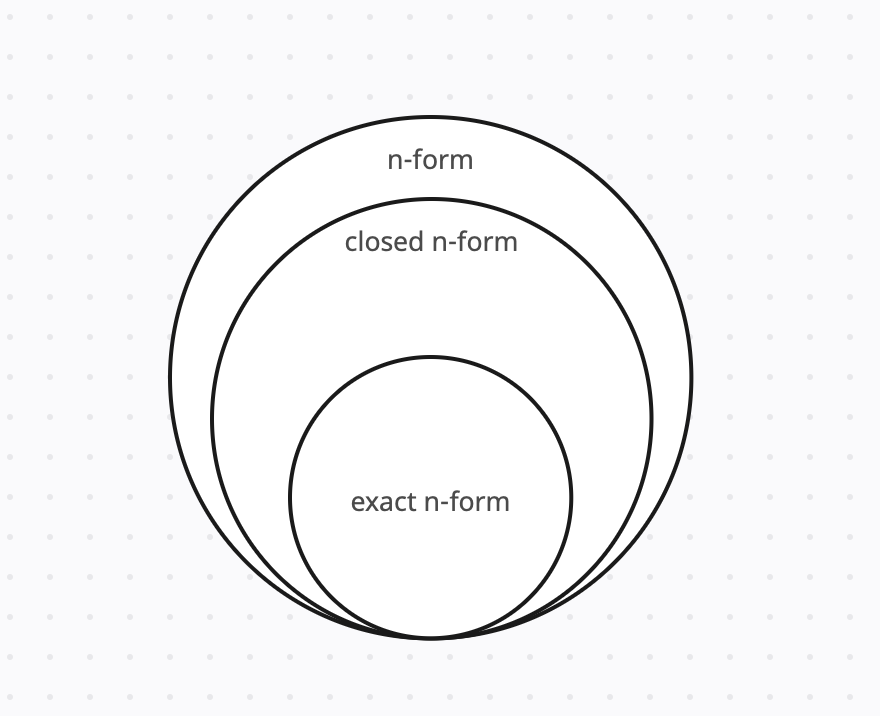
\includegraphics[height=8cm,width=14cm]{ednf}
   \end{minipage}
\end{center}
Thus, we may define the \textbf{De Rham cohomology group $H^k(M)$ in degree $k$ of  $M$} to be the quotient vector space 
\begin{align*}
H^k(M)\triangleq \frac{\set{\text{ closed $k$-th forms }}}{\set{\text{ exact $k$-th forms }}}
\end{align*}
By \myref{Theorem}{Cfz}, a 0-form is closed if and only if it is a constant, it follows from no 0-forms being exact that 
\begin{align*}
H^0(M)= \R
\end{align*}
if $M$ is connected. Note that the requirement of second countability make compact manifold have only finite amount of connected component. It follows that 
\begin{align*}
H^0(M)=\R^{\text{number  connected components of }M}
\end{align*}
It is clear that 
\begin{align*}
H^k(M)=\Omega^k(M)=0\text{ if }k>\operatorname{dim}M
\end{align*}
We may define a bilinear product $H^k(M)\times H^l(M)\to H^{k+l}(M)$ by 
\begin{align*}
[\alpha ][\beta ]\triangleq  [\alpha \wedge  \beta ]
\end{align*}
To see that this bilinear product is well-defined, compute 
\begin{align*}
  (\alpha + d\gamma )\wedge  (\beta  + d\delta)&= \alpha \wedge  \beta + \alpha \wedge  d \delta + d\gamma  \wedge  \beta  + d\gamma   \wedge  d\delta     \\
  &= \alpha \wedge  \beta  + (-1)^kd(\alpha \wedge  \delta )  + (-1)^{k-1}d (\gamma \wedge  \beta  )+d(\gamma  \wedge  d \delta )
\end{align*}
differing to $\alpha \wedge  \beta $ by some exact $k+l$-th form. If $F:M\rightarrow N$ is a smooth map, then we have a natural linear map $F^*:H^k(N)\rightarrow H^k(M)$ defined by 
\begin{align*}
F^* [\alpha ]\triangleq [F^* \alpha ]
\end{align*}
Again, this is well defined because 
\begin{align*}
F^*(\alpha +d \gamma )= F^* \alpha +d F^* \gamma  
\end{align*}
differing to $F^*\alpha $ by some exact $k$-form. 
\end{mdframed}
\begin{theorem}
\label{PPL}
\textbf{(Deformation invariance of De Rham Cohomology group)} Let $F:M\times  (-\epsilon  ,1+\epsilon )\rightarrow N$ be a smooth map. If we define $F_t:M\rightarrow N$ by 
\begin{align*}
F_t(x)\triangleq F(x,t)
\end{align*}
then for all $k\geq 0$
\begin{align*}
F_0^*=F_1^*
\end{align*}
\end{theorem}
\begin{proof}
Fix some closed form $\alpha \in \Omega^k(N)$. Locally, because $d\textbf{x}^1,\dots ,d\textbf{x}^m,dt$ form a basis for $T_p^*(M\times (-\epsilon , 1+\epsilon ) )$, by \myref{Theorem}{Boe} we may decompose $F^* \alpha $ into 
\begin{align*}
F^* \alpha  = \beta_t + \gamma_t \wedge  dt 
\end{align*}
where $\beta _t,\gamma _t\in \Omega^k (M)$. Write 
\begin{align*}
\beta _t= \sum_I B^I (\textbf{x}^1,\dots ,\textbf{x}^m,t)d\textbf{x}^I \text{ and } \gamma _t= \sum_I C^I (\textbf{x}^1,\dots ,\textbf{x}^m,t)d\textbf{x}^I
\end{align*}

Using \myref{Theorem}{Picw}, we may compute 
\begin{align*}
d(\beta _t + \gamma_t \wedge  dt )&=  d\Big( \sum_I B^I(\textbf{x}^1,\dots ,\textbf{x}^m,t)d\textbf{x}^I \Big) + d \Big(\sum_I C^I (\textbf{x}^1,\dots ,\textbf{x}^m,t)d\textbf{x}^I \Big) \wedge  dt  \\
&= \sum_I \Big[\sum_{j=1}^m \frac{ \partial B^I}{\partial \textbf{x}^j} d\textbf{x}^j \wedge    d\textbf{x}^I + \frac{\partial B^I}{\partial t}dt \wedge  d\textbf{x}^I    \Big] + \sum_I \sum_{j=1}^m \frac{\partial C^I}{\partial \textbf{x}^j}d\textbf{x}^j \wedge  d\textbf{x}^I \wedge  dt   \\
&= d_M \beta_t - \frac{\partial \beta _t}{\partial t} \wedge  dt+  (d_M \gamma_t) \wedge  dt 
\end{align*}
This with \myref{Theorem}{Pic} and the fact $\alpha $ is closed give us 
\begin{align*}
0=F^* d\alpha =dF^* \alpha = d(\beta _t + \gamma_t \wedge  dt ) =d_M\beta_t - \frac{\partial \beta _t}{\partial t}\wedge  dt + (d_M \gamma _t )\wedge  dt   
\end{align*}
This give us 
\begin{align*}
\frac{\partial \beta _t}{\partial t}= d_M \gamma_t
\end{align*}
Note that 
\begin{align*}
  F_t^* \alpha = \beta _t
\end{align*}
We then have 
\begin{align*}
  F_1^* \alpha -F_0^{*}\alpha &= \int_0^1 \frac{\partial \beta_t }{\partial t}dt \\
  &=\int_0^1 d_M \gamma_t dt =d_M \int_0^1 \gamma_t dt
\end{align*}
\end{proof}
\begin{corollary}
\label{PL}
\textbf{(Poincare Lemma)} Let $n,k\geq 1$. We have 
\begin{align*}
H^k(\R^n)=0 
\end{align*}
\end{corollary}
\begin{proof}
 Define $F:\R^n\times (-\epsilon ,1+\epsilon )\rightarrow \R^n$ by 
  \begin{align*}
  F(\textbf{x},t)\triangleq t\textbf{x}
  \end{align*}
so that 
\begin{align*}
F_0\text{ is the zero map and $F_1$ is the identity map }
\end{align*}
Now, because for $k\geq 1$
\begin{align*}
  &F_0^*:\Omega^k(\R^n)\rightarrow \Omega^k(\R^n)\text{ is a zero map } \\
  \text{ and }&F_1^* :\Omega^k(\R^n)\rightarrow \Omega^k (\R^n)\text{ is the identity map }
\end{align*}
we have 
\begin{align*}
&F_0^*:H^k(\R^n)\rightarrow H^k(\R^n)\text{ is a zero map } \\
  \text{ and }&F_1^*:H^k(\R^n)\rightarrow H^k(\R^n)\text{ is the identity map }
\end{align*}
\myref{Theorem}{PPL} states that $F_0^*=F_1^*$. It then follows that $H^k(\R^n)=0$.
\end{proof}
\begin{mdframed}
The same argument can be used to show 
\begin{align}
\label{hkm}
H^k(M\times \R^m)\cong  H^k(M)
\end{align}
for $k\geq 0$ by setting 
\begin{align*}
F(p,\textbf{x},t)\triangleq (p,t \textbf{x})
\end{align*}
\end{mdframed}
\begin{mdframed}
We now compute $H^k(S^1)$ by another method. Again note that $H^0(S^1)\cong  \R$ because $S^1$ is connected and  $H^k(S^1)\cong 0$ for $k\geq 2$ because $\operatorname{dim}S^1=1$. Recall that $S^1\cong  \R \setminus \Z$ where $\R \setminus \Z$ is given the smooth structure 
\begin{align*}
  \begin{cases}
\phi_0: \set{[x]:x\in (0,1)}  \rightarrow (0,1) \\
\phi_0 ( \pi ^{-1}(x))\triangleq x
  \end{cases} \text{ and }\begin{cases}
\phi_1: \set{[x]:x\in (\frac{-1}{2},\frac{1}{2})}  \rightarrow (-\frac{1}{2},\frac{1}{2}) \\
\phi_1 ( \pi ^{-1}(x))\triangleq x
  \end{cases}
\end{align*}
We claim the $1$-form  $\alpha \in \Omega^1 (\R \setminus \Z)$ defined by 
\begin{align*}
\alpha \triangleq \begin{cases}
  dx_0 \text{ on }\set{[x]: x \in (0,1)} \\
  dx_1\text{ on }\set{[x]:x \in (\frac{-1}{2}, \frac{1}{2})}
\end{cases}
\end{align*}
is well-defined, where $x_0: \set{[x]: x \in (0,1)}\rightarrow (0,1),x_1 : \set{[x]:x \in (\frac{-1}{2}, \frac{1}{2})}\rightarrow  (\frac{-1}{2}, \frac{1}{2})$ is defined by 
\begin{align*}
x_0\triangleq \phi_0   \text{ and }x_1 \triangleq \phi_1
\end{align*}
This is true because the area where two charts overlaps have two connected components, and $x_0,x_1$ take the same value on one of them while taking values different by constant $1$ on another. Also note that $\alpha $ is clearly non-zero, so we have shown $\Omega^1 (\R \setminus \Z)\neq 0$. \\

Note that $\alpha $ is not exact since if $\alpha = d\gamma $ for some $\gamma \in \Omega^0(\R \setminus \Z)$ then $\gamma $ on $\set{[x]: x \in (0,1)}$ must have the same action as $x_0$, which is impossible since this make  $\gamma $ discontinuous at end-point. On the other hand, suppose $\beta  \in \Omega^1 (\R \setminus \Z)$. Write in local coordinate 
\begin{align*}
\beta  (x)=g(x)dx\text{ on }\set{[x]:x \in (0,1)}
\end{align*}
Set $f\in \Omega^{1}(\R \setminus \Z)$ by 
\begin{align*}
f(x)\triangleq \int_0^x g(s)ds - \Big( \int_0^1 g(s)ds \Big)x \text{ on } \set{[x]:x \in (0,1)}
\end{align*}
It follows that 
\begin{align*}
\beta = \Big( \int_0^1 g(s)ds \Big)\alpha + df
\end{align*}
We have shown $H^1(S^1)=\R$
\end{mdframed}
\begin{theorem}
\textbf{(De Rham Cohomology of $S^n$)} For $n>0$ 
 \begin{align*}
H^k (S^n) \cong \begin{cases}
  \R & \text{ if $k=0\text{ or }n$ }\\
  0& \text{ if otherwise }
\end{cases}
\end{align*}
\end{theorem}
\begin{proof}
The case of $n=1$ have been proved in the above paragraph. We first prove 
\begin{align*}
\vi{H^1(S^2)\cong  0}
\end{align*}
Define  
 \begin{align*}
 U \triangleq S^2 \setminus \overline{B_\epsilon (N)} \text{ and }V \triangleq S^2 \setminus \overline{B_\epsilon (S)}
 \end{align*}
By means of stereographic projection, we know $U$ and  $V$ are both diffeomorphic to an open ball in  $\R$. Let $\alpha \in \Omega^1(S^2)$ be a closed $1$-form.  By \customref{PL}{Poincare Lemma}, $\alpha |_U$ and $\alpha |_V$ are both exact. Write 
\begin{align*}
\alpha = du \text{ on }U\text{ and }\alpha =dv\text{ on }V
\end{align*}
where $u\in \Omega^{0}(U),v \in \Omega^{0}(V)$ are two zero-forms. Compute 
\begin{align*}
d(u-v)=\alpha -\alpha =0\text{ on }U\cap V
\end{align*}
This implies $u-v \in \Omega^{0}(U \cap V)$ are closed. It then follows from $U \cap V$ being connected that $u-v\in \Omega^0(U \cap V)$ is constant. Therefore, if we define $\gamma \in \Omega^0(S^1)$ by 
\begin{align*}
\gamma  \triangleq \begin{cases}
  u& \text{ on  }U\\
  v+c&\text{ on }V
\end{cases}
\end{align*}
where $c\equiv u-v$ on $U \cap V$, then $\gamma $ is well-defined. It is easily seen that $\alpha = d\gamma $. $\vdone$\\

We now prove 
\begin{align*}
\blue{H^2(S^2)\cong  \R}
\end{align*}
Again, define 
 \begin{align*}
 U \triangleq S^2 \setminus \overline{B_\epsilon (N)} \text{ and }V \triangleq S^2 \setminus \overline{B_\epsilon (S)}
 \end{align*}
By means of stereographic projection, we know $U$ and  $V$ are both diffeomorphic to an open ball in  $\R^2$. Let $\alpha \in \Omega^2(S^n)$ be a closed $2$-form. By \customref{PL}{Poincare Lemma}, $\alpha |_U, \alpha |_V$ are both exact. Write 
\begin{align*}
\alpha = du \text{ on }U\text{ and }\alpha =dv\text{ on }V
\end{align*}
where $u\in \Omega^{1}(U),v \in \Omega^{1}(V)$ are two $1$-forms. Compute 
\begin{align*}
d(u-v)=\alpha -\alpha =0\text{ on }U\cap V
\end{align*}
This implies $u-v\in \Omega^{1}(U \cap V)$ are closed. Compute by \myref{Equation}{hkm} 
\begin{align*}
H^{1}(U \cap V)\cong  H^{1}(S^{1}\times \R)\cong  H^{1}(S^{1})\cong \R
\end{align*}
Let $[\omega]\in H^1(U \cap V)$ be non-trivial. We then see 
\begin{align*}
u-v=c \omega + dw 
\end{align*}
for some unique $c \inr$ and $w\in \Omega^0(U \cap V)$. We now show that \olive{such $c$ only depends on $\alpha $, independent of choice of  $u,v$}.   




We may now define a linear map $H^2(S^2)\rightarrow \R$ by 
\begin{align*}
\alpha \mapsto c_\alpha 
\end{align*}

\end{proof}
\section{Orientation}
\begin{abstract}
  This section gives an \customref{EDO}{equivalent definitions for orientation} and constructs \customref{Svf}{the standard volume form for $S^n$}. In this section, $M$ is always a $m$-dimensional smooth manifold  
\end{abstract}
\begin{mdframed}
Let $(U,\textbf{x}),(V,\textbf{y})$ be two charts for $M$. If 
\begin{align*}
  \operatorname{det} \Big(\frac{\partial \textbf{y}^i}{\partial \textbf{x}^j} \Big)>0\text{ everywhere on }U \cap V
\end{align*}
we say their transition function is \textbf{orientation preserving}. We say an atlas $\mathcal{U}$ for  $M$ is  \textbf{oriented atlas} if all transition functions for $\mathcal{U}$ is orientation preserving. A maximal oriented atlas for $M$ is said to be an  \textbf{orientation} of $M$. If $M$ admits an oriented atlas, we say  $M$ is  \textbf{orientable}; moreover, if we say $M$ is an  \textbf{oriented manifold}, we mean that $M$ is equipped with a maximal oriented atlas.\\

By a \textbf{volume form on $M$}, we mean a top-degree differential form $\omega \in \Omega^m(M)$ such that $\omega$ is non-zero everywhere. On the space of volume forms, we may define an equivalence relation by relating two volume forms $\omega,\omega'$ together if there exists some positive zero-form $f\in \Omega^0(M)$ such that  $\omega'=f \omega$.\\


We may now prove the equivalency of two definitions of orientation.  
\end{mdframed}
\begin{theorem}
\label{EDO}
\textbf{(Equivalent Definition of Orientation)} Let $M$ be a smooth manifold. There exists a one-to-one correspondence between the set of orientation of $M$ and the set of equivalence class of volume forms. 
\end{theorem}
\begin{proof}
Let $\omega$ be a volume form. By changing $\textbf{x}^1$ to $-\textbf{x}^1$ if necessary, we may find an atlas $\mathcal{U}$ such that 
\begin{align}
\label{vu}
f>0\text{ when we write }\omega= f(\textbf{x}) \ld^1 \wedge  \cdots \wedge  \ld ^n  \text{ on }U
\end{align}
for all $(U,\textbf{x})\in \mathcal{U}$. If on another chart $(V,\textbf{y})\in \mathcal{U}$, we write 
\begin{align*}
\omega= g(\textbf{y})\tilde{\ld }^1 \wedge  \cdots \wedge  \tilde{\ld }^n  \text{ on }V
\end{align*}
by \myref{Equation}{ldi}, we may compute 
\begin{align*}
f(\textbf{x})\ld ^1 \wedge  \cdots \wedge   \ld ^n=\omega&= g(\textbf{y}) \tilde{\ld } ^1 \wedge  \cdots \wedge \tilde{\ld } ^n   \\
&= g(\textbf{y}(\textbf{x})) \operatorname{det}\Big( \frac{\partial \textbf{y}^i}{\partial \textbf{x}^j} \Big) \ld ^1 \wedge  \cdots \wedge  \ld ^n  \text{ on }U\cap V
\end{align*}
It follows from $f,g$ are both positive that $\operatorname{det}\Big( \frac{\partial \textbf{y}^i}{\partial \textbf{x}^j} \Big)>0$. We have shown $\mathcal{U}$ is an oriented atlas. Direct computation with \myref{Equation}{ldi} shows that if $\omega'$ is a volume form equivalent to $\omega$, then the oriented atlas $\mathcal{U}'$ induced by the same procedure is consistent with $\mathcal{U}$. We have constructed a function  $F$ that maps the set of equivalence class of volume forms into the set of orientation of  $M$. Note that, again, direct computation with \myref{Equation}{ldi} shows that $F$ is one-to-one. \\

It remains to show $F$ is onto. Let $(U_\alpha )$ be a maximal oriented atlas, and let \customref{Smooth manifolds always admit smooth partition of unity}{$(\phi_\alpha )$ be a partition of unity subordinate to $(U_\alpha )$}. Define $\omega \in \Omega^n(M)$ by 
\begin{align*}
\omega \triangleq \sum_{\alpha } \phi_\alpha \ld ^1_\alpha \wedge  \cdots \wedge  \ld _\alpha ^n  
\end{align*}
Note that $\omega$ is well-defined because $(\phi_\alpha )$ is locally finite. Let $p \in M$. To see $\omega$ is indeed non-vanishing, let $(U_{\alpha _1},\textbf{x})$ be a chart containing $p$, and compute on an neighborhood around $p$ 
 \begin{align*}
\omega&= \sum_{\alpha :\phi_\alpha (p)>0} \phi_\alpha d\textbf{y}^1_\alpha \wedge  \cdots \wedge  d\textbf{y}^n_\alpha    \\
&= \sum_{\alpha :\phi_\alpha (p)>0} \phi_\alpha  \operatorname{det}\Big( \frac{\partial \textbf{y}^i_\alpha  }{\partial \textbf{x}^j } \Big) d\textbf{x}^1 \wedge  \cdots \wedge   d\textbf{x}^n\neq 0
\end{align*} 
This implies that $\omega$ is a volume form satisfying \myref{Equation}{vu}. In other words, $F$ maps  $[\omega]$ to $(U_\alpha )$. We have shown $F$ is indeed onto.  
\end{proof}
\begin{mdframed}
Because of \myref{Theorem}{EDO}, if $M$ is oriented with oriented atlas $\mathcal{U}$ and  $\omega$ is a volume form such that 
\begin{align*}
f>0\text{ when we write }\omega= f(\textbf{x}) \ld^1 \wedge  \cdots \wedge  \ld ^n  \text{ on }U\text{ for all }U \in \mathcal{U}
\end{align*}
we say $\omega$ is a \textbf{positively oriented volume form}. 
\end{mdframed}
\label{Svf}
\begin{Example}{\textbf{(Standard volume form of $S^n$)}}{}
\vspace{0.8cm}
Let $f:\R^{n+1}\rightarrow \R$ be a smooth map, and $M\subseteq \R^{n+1}$ be a regular level set. By \customref{Regular Level Set Theorem}{regular level set theorem}, $M$ is an embedded submanifold of $\R^{n+1}$. Let $p \in M$. Because $p$ is a regular point, we know 
\begin{align*}
\frac{\partial f}{\partial \textbf{x}^i}(p) \neq 0\text{ for some }i
\end{align*}
then by \customref{IpFT}{implicit function theorem} and uniqueness of smooth structure, we have some chart $(U,\phi)$ around $p$ such that 
\begin{align*}
\phi (\textbf{x}^1,\dots ,\textbf{x}^n)= (\textbf{x}^1,\dots , \widehat{\textbf{x}}^i,\dots ,\textbf{x}^{n+1})
\end{align*}
and 
\begin{align*}
\frac{\partial f}{\partial \textbf{x}^i}\neq 0\text{ on }U
\end{align*}
Therefore, we may define a non-vanishing $n$-form $\omega$ on $U$ by  
\begin{align}
\label{ojh}
\omega\triangleq  (-1)^i \Big(\frac{\partial f}{\partial \textbf{x}^i}\Big)^{-1}  d\textbf{x}^1\wedge \cdots  \wedge  \widehat{d \textbf{x}}^i \wedge  \cdots \wedge  d \textbf{x}^{n+1}
\end{align}
To see $\omega$ is globally well-defined, first observe that   because $f$ is constant on  $M$, globally we have 
 \begin{align}
\label{0df}
0=\sum_{k} \frac{\partial f}{\partial \textbf{x}^k}d\textbf{x}^k
\end{align}
Now, if $(V,\psi)$ is a similarly defined chart with 
\begin{align*}
\phi (\textbf{x}^1,\dots ,\textbf{x}^n)= (\textbf{x}^1,\dots ,\widehat{\textbf{x}}^j,\dots ,\textbf{x}^{n+1}) 
\end{align*}
and 
\begin{align*}
\frac{\partial f}{\partial \textbf{x}^j}\neq 0\text{ on }V
\end{align*}
such that $V \cap U\neq \varnothing$, we may compute by \myref{Equation}{0df} that 
\begin{align*}
d\textbf{x}^j = - \Big( \frac{\partial f}{\partial \textbf{x}^j} \Big)^{-1} \sum_{k\neq j} \frac{\partial f}{\partial \textbf{x}^j}  d\textbf{x}^k\text{ on }U \cap V
\end{align*}
Therefore, the expression of $\omega$ in \myref{Equation}{ojh} on $V \cap U$ is equal to 
\begin{align*}
  \omega= (-1)^j \Big( \frac{\partial f}{\partial \textbf{x}^j} \Big)^{-1}d\textbf{x}^1 \wedge  \cdots \wedge  \widehat{d \textbf{x}}^j \wedge  \cdots \wedge  d\textbf{x}^{n+1}    
\end{align*}
We have shown $\omega$ is globally well-defined. Now, if we let $f(\textbf{x})\triangleq \abso{\textbf{x}}^2$ and let $f(M)=1$, we see $M=S^n$ and  
 \begin{align*}
\omega= \frac{(-1)^i}{2\textbf{x}^i} d\textbf{x}^1 \wedge  \cdots \wedge \widehat{d \textbf{x}}^i \wedge \cdots \wedge  d\textbf{x}^{n+1}    
\end{align*}
on $\set{\textbf{x} \in S^n: \textbf{x}^i \neq 0}$. We call this $\omega$ the \textbf{standard volume form on $S^n$}. 
\end{Example}
\begin{mdframed}
Because the $m$-th exterior powers of $T_p^*M$ are 1-dimensional, for each pair of volume forms  $\omega,\omega' \in \Omega^m(M)$, there exists some $f:M\rightarrow \R^*$ such that $\omega'=f \omega$. Charts by charts, one can check that $f\in \Omega^0(M)$ is indeed smooth. Define $g:\R^*\rightarrow \set{0,1}$ by 
  \begin{align*}
  g(x)\triangleq \begin{cases}
    1& \text{ if $x>0$ }\\
    0& \text{ if $x<0$ }
  \end{cases}
  \end{align*}
Because $g$ is continuous, we know  $g \circ f: M\rightarrow \set{0,1}$ is continuous. It then follows that if $M$ has  $n$ connected components, then there are $2^n$ orientation on  $M$. 
\end{mdframed}
\section{Integration on Manifold}
\begin{abstract}
In this section, we introduce the idea of integration on smooth manifold and prove  \customref{HBT}{the hairy ball theorem} for smooth vector field and that \customref{rpin}{$\RP^n$ is not orientable for even  $n$}
\end{abstract}
\begin{mdframed}
Let $M$ be an oriented manifold and  $\omega \in \Omega^m(M)$ be a top-degree form with compact support.  Because $M$ is oriented and $\omega$ is of compact support, we may find a finite set of charts $U_1,\dots ,U_N$ such that $\operatorname{supp}\omega \subseteq U_1 \cup \cdots \cup U_N$ and $f_i$ share the same sign if we write on each chart  
\begin{align*}
\omega|_{U_i }= f_i (\textbf{x})\ld_i^1 \wedge  \cdots \wedge  \ld_i^m
\end{align*}
Let $\phi_1,\dots ,\phi_N$ be a smooth partition of unity subordinated to $U_1,\dots ,U_N$. We define the integral of $\omega$ on $M$ to be 
 \begin{align*}
\int_M \omega\triangleq \sum_{i=1}^N \int_{\R^m} \phi_i f_i (\textbf{x}) 
\end{align*}
To show that the definition is independent of choice of the finite covers and partition of unity, let $\tilde{U}_j$ be a another finite cover and $\tilde{\phi}_j$ a subordinating partition of unity, and check 
\begin{align*}
\sum_j \int_M \tilde{\phi}_j \omega= \sum_{i,j} \int_M \tilde{\phi}_j \phi_i \omega  = \sum_i \int_M \phi_i \omega
\end{align*}
\end{mdframed}
\begin{theorem}
\label{SCST}
\textbf{(Special Case of Stoke's Theorem)} Let $M$ be oriented and  $\omega\in \Omega^{m-1}(M)$ be of compact support. We have 
\begin{align*}
\int_M d\omega=0
\end{align*}
\end{theorem}
\begin{proof}
Again, let $\phi_i$ be a partition of unity subordinated to a positively oriented finite set of charts. On each chart, we may write 
\begin{align*}
\phi_i \omega= \sum_{n=1}^m (-1)^{n+1} a_n \ld^1 \wedge  \cdots \wedge \widehat{\ld }^n \wedge  \cdots \wedge \ld^m    
\end{align*}
Compute 
\begin{align*}
d(\phi_i \omega)= \sum_{n=1}^m \frac{\partial a_n}{\partial \textbf{x}^n} \ld ^1 \wedge  \cdots \wedge \ld^m   
\end{align*}
It then follows from each $a_n$ is of compact support that 
 \begin{align*}
\int_M d\omega= \sum_i \int_M d(\phi_i \omega)=0
\end{align*}
\end{proof}
\begin{mdframed}
Immediately, following from \customref{SCST}{special case of Stoke's theorem}, we see that if $M$ is compact and orientable, then 
 \begin{align*}
H^m(M)\neq 0
\end{align*}
since if $\alpha \in \Omega^m(M)$ is a positively oriented volume forms, then 
\begin{align*}
\int_M \alpha  >0
\end{align*}
which implies $\alpha $ is not exact. 
\end{mdframed}
\begin{theorem}
\label{rpin}
\textbf{($\RP^n$ is not orientable for even  $n$)} Define an equivalence relation on $\R^{n+1}\setminus \set{\textbf{0}}$ by 
\begin{align*}
\textbf{x}\sim \textbf{y}\text{ if }\textbf{x}=\ld  \textbf{y}\text{ for some }\ld \inr
\end{align*}
Let $\pi $ be the quotient map and $\RP^n$ be the quotient space. If we give $\RP^n$ the atlas 
\begin{align*}
[\textbf{x}_1 ,\dots ,\textbf{x}_{n+1}]\mapsto  \Big(\frac{\textbf{x}_1}{\textbf{x}_i}, \dots , \frac{\textbf{x}_{i-1}}{\textbf{x}_i},\frac{\textbf{x}_{i+1}}{\textbf{x}_i}, \dots ,\frac{\textbf{x}^{n+1}}{\textbf{x}^i}\Big) 
\end{align*}
and $n$ is even, then  $\RP^n$ is not orientable. 
\end{theorem}
\begin{proof}
We first show that
\begin{center}
   \begin{minipage}{0.9\linewidth}  
     \olive{$\pi  : S^n \rightarrow \RP^n $ is a smooth immersion}. 
   \end{minipage}
\end{center}
Define $U\triangleq \set{\textbf{x}\in S^n: \textbf{x}_1>0}$ and $\phi : U\rightarrow \R^n$ by 
\begin{align*}
\phi (\textbf{x})\triangleq (\textbf{x}_2 ,\dots , \textbf{x}_n)
\end{align*}
Compute 
\begin{align*}
\psi \circ \pi  \circ  \phi ^{-1} (\textbf{x}_2 ,\dots ,\textbf{x}_{n+1})=  \Big(\frac{\textbf{x}_2}{\textbf{x}_1},\dots , \frac{\textbf{x}_{n+1}}{\textbf{x}_1}\Big)
\end{align*}
We have shown $\pi $ is indeed smooth. To see $\pi _{*,p}$ is invertible everywhere, observe that $\psi \circ \pi  \circ   \phi^{-1}$ have the action 
\begin{align*}
\textbf{y}\mapsto  \frac{\textbf{y}}{\sqrt{1- \abso{\textbf{y}}^2} }
\end{align*}
which has a left inverse 
\begin{align*}
\textbf{y}\mapsto \frac{\textbf{y}}{\sqrt{1+ \abso{\textbf{y}}^2} }
\end{align*}
One can check from definition of $\pi $ that this left inverse is indeed an inverse. More precisely, we have established a diffeomorphism between $U$ and $\pi  (U)$. Therefore, $\pi$ is a local diffeomorphism. This implies $\pi _{*,p}$ is invertible everywhere. $\odone$ \\

 Let $\omega \in \Omega^n (S^n)$ be the \customref{Svf}{standard volume form of $S^n$}. Define a smooth diffeomorphism $\sigma :S^n\rightarrow S^n$ by 
\begin{align*}
\sigma (\textbf{x})\triangleq - \textbf{x}
\end{align*}
We now show 
\begin{align}
\label{sgw}
  \vi{\sigma^* \omega = - \omega}
\end{align}
Compute on $\set{\textbf{x} \in S^n : \textbf{x}_i \neq 0} $
\begin{align*}
  \sigma^* \omega &=  \sigma^*  \Big[\frac{(-1)^i}{2\textbf{x}_i} d\textbf{x}_1 \wedge  \cdots \wedge \widehat{d \textbf{x}_i} \wedge \cdots \wedge  d\textbf{x}_{n+1}  \Big] \\
  &= \frac{(-1)^i}{-2\textbf{x}_i}d(-\textbf{x}_1)\wedge  \cdots \wedge  d(-\textbf{x}_{i-1}) \wedge  d(-\textbf{x}_{i+1}) \wedge  \cdots \wedge   d(-\textbf{x}_{n+1})    \\
  &=(-1)^{n-1} \omega=-\omega 
\end{align*}
Repeating the same computation on $\textbf{x}_j \neq 0$, we see that, indeed, $\sigma^* \omega= -\omega$ globally. $\vdone$\\


\As{$\theta \in \Omega^n (\RP^n)$ is a volume form}. Because $\pi$ is an immersion, we know $\pi ^* \theta \in \Omega^n (S^n)$ is also a volume form. Therefore, we may define an no-where-zero $f\in \Omega^0(S^n)$ by 
\begin{align*}
f\triangleq \frac{\pi ^* \theta}{\omega }
\end{align*}
It is clear that $\pi \circ \sigma= \pi  $. Therefore, 
\begin{align*}
  f\omega= \pi ^* \theta= (\pi  \circ  \sigma)^* \theta= \sigma^* \pi ^* \theta= \sigma^* (f \omega)= -(f \circ \sigma)\omega 
\end{align*}
This give us 
\begin{align*}
f(\textbf{x})=-f(-\textbf{x})\text{ for all }\textbf{x}\in S^n
\end{align*}
This is impossible, since the fact that $S^n$ is connected implies  $f$ have the same sign everywhere. \CaC 
\end{proof}
\begin{theorem}
\label{HBT}
\textbf{(Hairy Ball Theorem in Differential Geometry)} Let  $X\in \mathfrak{X}(S^{2m})$ be a smooth vector field. 
\begin{align*}
\text{ There exists some $p  \in S^{2m}$ such that }X_p=0
\end{align*}
\end{theorem}
\begin{proof}
\As{$X$ is non-vanishing}. Obviously, we may identify each $T_\textbf{x}S^{2m}$ as a $2m$-dimensional subspace of  $\R^{2m+1}$ orthogonal to $\textbf{x}$. This way, $X$ is smooth function that maps  $S^{2m}$ into $\R^{2m+1}$ such that 
\begin{align*}
X(\textbf{x})\cdot \textbf{x}=0\text{ for all }\textbf{x} \in S^{2m}
\end{align*}
Because the normalizing function $\textbf{x}\mapsto \frac{\textbf{x}}{\abso{\textbf{x}}}$ is smooth, if we define $\widehat{X}\in \mathfrak{X}(S^{2m})$ by 
\begin{align*}
\widehat{X}_\textbf{x}\triangleq \frac{X_\textbf{x}}{\abso{X_\textbf{x}}}
\end{align*}
then $\widehat{X}$ is indeed smooth. Define $F_t:S^{2m}\rightarrow S^{2m}$ by 
\begin{align*}
F_t(\textbf{x})\triangleq (\cos t)\textbf{x}+ (\sin t)\widehat{X}_\textbf{x}
\end{align*}
Tedious computations shows that $F:S^{2m}\times \R \rightarrow S^{2m}$ is indeed smooth. Compute 
\begin{align*}
F_0(\textbf{x})=\textbf{x}\text{ and }F_\pi  (\textbf{x})=-\textbf{x}\text{ for all }\textbf{x}\in S^{2m}
\end{align*}
Let $\omega \in \Omega^{2m}(S^{2m})$ be the \customref{Svf}{standard volume form}. By \myref{Equation}{sgw} proved in \myref{Theorem}{rpin}, we have 
\begin{align*}
F_0(\omega)=\omega\text{ and }F_\pi  (\omega)=-\omega
\end{align*}
It then follows from \customref{PPL}{deformation invariance of De Rham cohomology group} that $\omega$ is exact. This cause a contradiction, since \customref{SCST}{special case of Stoke's theorem} says that exact top-form $\omega$ on $S^{2n}$, which is compact, must have 
\begin{align*}
\int_M \omega =0
\end{align*}
while the fact $\omega$ is the standard volume form implies 
\begin{align*}
\int_M \omega> 0 \tCaC
\end{align*}
\end{proof}
\section{Stoke's Theorem}
\begin{abstract}

\end{abstract}
\begin{mdframed}
In this section, we use  $\H^n$ to denote the upper-half space of $\R^n$
\begin{align*}
\H^n \triangleq \set{\textbf{x}\in \R^n: \textbf{x}^n \geq 0}
\end{align*}
By a $n$-dimensional topological manifold with boundary, we mean a second-countable and Hausdorff topological space $M$ such that for all $p \in M$, there exists some neighborhood $U$ around  $p$ homeomorphic to some open subsets of  $\H^n$. By invariance of domain, a non-trivial Theorem in algebraic topology, one can deduce that if $p$ is mapped by some chart into $\partial \H^n$, then all charts map $p$ into  $\partial \H^n$. Therefore, we may distinguish between the \textbf{interior $M^\circ $ and boundary $\partial M$ of $M$}.  \\

It is clear that $M^\circ $ and $\partial M$ when endowed with subspace topology from $M$, they are respectively a $n$-dimensional topological  manifold and a $(n-1)$-dimensional topological manifold. Let $f$ be a function that maps $E\subseteq \H^n$ into $\R^n$, where $E$ is open in  $\H^n$ and contain $p \in \partial \H^n$, we say $f$ is smooth at $p$ if there exists some smooth function $\widehat{f}:B_\epsilon (p)\rightarrow \R^n$ such that 
\begin{align*}
\widehat{f}\equiv f \text{ on }E\cap B_\epsilon (p)
\end{align*}
With this in mind, it make sense for us to talk about \textbf{smooth manifold with boundary}. \\

Let $p \in \partial M$ and $(U,\phi)$ be a chart around $p$. Because
\begin{align*}
T_pM\cong  T_p U\cong  T_{\phi (p)}\phi (U)\cong  T_{\phi (p)} \H^n \cong  T_{\phi (p)}\R^n
\end{align*}
we see $T_pM$ is also  $n$-dimensional, where the last isomorphism is given by the derivative of inclusion map $\diota: \H^n\rightarrow \R^n $. (Lemma 3.11 in Lee) 
\end{mdframed}
\begin{theorem}
\textbf{(Induced orientation on boundary)} If $\mathcal{U}$ is an oriented atlas for $M$, then its restriction 
\begin{align*}
\mathcal{U}'\triangleq \bset{(U\cap \partial M,\phi |_{U \cap \partial M}): (U,\phi) \in \mathcal{U}}
\end{align*}
is an oriented atlas for $\partial M$. 
\end{theorem}
\begin{proof}
Let $(U,\textbf{x}),(V,\textbf{y}) \in \mathcal{U}$. Because 
\begin{align*}
\textbf{y}^n (\textbf{x}^1,\dots ,\textbf{x}^{n-1},0)=0
\end{align*}
we know 
 \begin{align*}
\frac{\partial \textbf{y}^n}{\partial \textbf{x}^{i}}=0,\frac{\partial \textbf{y}^n}{\partial \textbf{x}^n}>0\text{ for $i<n$ on }\partial M
\end{align*}
Then because the Jacobian $J_M$ of the transition function between $\textbf{x},\textbf{y}$ has the form 
\begin{align*}
\begin{vmatrix} 
  \frac{\partial \textbf{y}^1}{\partial \textbf{x}^1} & \cdots & \frac{\partial \textbf{y}^1}{\partial \textbf{x}^{n-1} & \frac{\partial \textbf{y}^1}{\partial \textbf{x}^n}} \\
  \vdots & \ddots & \vdots & \vdots  \\
  \frac{\partial \textbf{y}^{n-1}}{\partial \textbf{x}^1} & \cdots & \frac{\partial \textbf{y}^{n-1}}{\partial \textbf{x}^{n-1}} & \frac{\partial \textbf{y}^{n-1}}{\partial \textbf{x}^n} \\
  0 & \cdots & 0 & \frac{\partial \textbf{y}^n}{\partial \textbf{x}^n}
\end{vmatrix}\text{ on }\partial M
\end{align*}
we see that the Jacobian $J_{\partial M}$ of the transition function between the restricted $\textbf{x},\textbf{y}$ is 
\begin{align*}
\begin{vmatrix} 
  \frac{\partial \textbf{y}^1}{\partial \textbf{x}^1} & \cdots & \frac{\partial \textbf{y}^1}{\partial \textbf{x}^{n-1}} \\ 
  \vdots & \ddots & \vdots  \\
  \frac{\partial \textbf{y}^{n-1}}{\partial \textbf{x}^1} & \cdots & \frac{\partial \textbf{y}^{n-1}}{\partial \textbf{x}^{n-1}}  
\end{vmatrix} = \frac{J_M}{\frac{\partial \textbf{y}^n}{\partial \textbf{x}^n}}>0
\end{align*}
\end{proof}
\begin{mdframed}
Note that if a positively oriented volume form $\omega$ has the expression 
\begin{align*}
f(\textbf{x}) d\textbf{x}^1 \wedge  \cdots \wedge  d\textbf{x}^n  
\end{align*}
then its pullback $\diota^*\omega $ to the boundary by \textbf{stoke convention} have the expression 
\begin{align}
\label{-1n}
  (-1)^n f(\textbf{x})d\textbf{x}^1 \wedge  \cdots \wedge  d\textbf{x}^{n-1}  
\end{align}
\end{mdframed}
\begin{theorem}
\textbf{(Stoke's Theorem)} Let $M$ be an oriented  $n$-dimensional manifold with  boundary $\partial M$, and let $\omega \in \Omega^{n-1}(M)$ be of compact support. We have 
\begin{align*}
\int_M d\omega = \int_{\partial M} \omega 
\end{align*}
where the restriction of $\omega$ on $\partial M$ should be considered as the pullback $\diota^*\omega $ of $\diota: \partial M\rightarrow M $. 
\end{theorem}
\begin{proof}
Let $\set{U_\alpha }$ be an open cover, and let $\set{\rho_\alpha }$ be a subordinate partition of unity. Therefore, we may write 
\begin{align*}
\int_M d\omega= \sum_{i=1}^N \int_M \rho_i d\omega= \sum_{i=1}^N \int_M d(\rho_i \omega)
\end{align*}
Fix $i$. Write   
\begin{align}
\label{fi}
\rho_i \omega= \sum_{j=1}^n (-1)^{j-1}a_j d\textbf{x}^1 \wedge  \cdots \wedge  \widehat{d \textbf{x}^j}  \wedge  \cdots \wedge   d\textbf{x}^n 
\end{align}
And compute 
\begin{align*}
d (\rho_i \omega)= \sum_{j=1}^n \frac{\partial a_j}{\partial \textbf{x}^j} d\textbf{x}^1 \wedge  \cdots \wedge  d\textbf{x}^n  
\end{align*}
If $U_i\cap  \partial M= \varnothing$, then we may use Fubini's Theorem and Fundamental Theorem of Calculus to conclude 
\begin{align*}
\int_M d(\rho_i \omega)=0 
\end{align*}
If  $U_i \cap \partial M \neq \varnothing$,  by \myref{Equation}{-1n} and \myref{Equation}{fi}, we may observe 
\begin{align*}
\diota^* (\rho_i \omega) = - a_n d\textbf{x}^1 \wedge  \cdots \wedge  d\textbf{x}^{n-1}  
\end{align*}
And again use Fubini's Theorem and Fundamental Theorem of Calculus to compute 
\begin{align*}
\int_M d(\rho_i \omega)=  \int_{\textbf{x}^n \geq 0} \frac{\partial a_n}{\partial \textbf{x}^n} &= \int_{\R^{n-1}} a_n(\textbf{x}^1,\dots ,\textbf{x}^n)\Big|_{\textbf{x}^n=0}^{\infty } \\
&=-\int_{\R^{n-1}} a_n (\textbf{x}^1,\dots ,\textbf{x}^{n-1},0) \\
&=\int_{\partial M} \rho_i \omega
\end{align*}
This finishes the proof.
\end{proof}
\begin{theorem}
\textbf{(Brouwer's fixed point Theorem)} If 
\end{theorem}
\begin{proof}

\end{proof}
\begin{theorem}
\textbf{(Top De Rham cohomology group of oriented compact connected manifold)} If $M$ is a $n$-dimensional oriented compact connected manifold, then 
 \begin{align*}
H^n(M)\cong  \R
\end{align*}
\end{theorem}
\begin{proof}

\end{proof}
\section{Degree Theory}
\begin{theorem}
\textbf{(Degree of a Smooth Map)} Suppose $M$ and  $N$ are compact, connected, oriented, smooth manifold of dimension  $n$, and  $F:M\rightarrow N$ is a smooth map. There exists a unique integer $k$, called the  \textbf{degree of $F$}, that satisfies both the following conditions 
\begin{enumerate}[label=(\alph*)]
  \item For every smooth $n$-form  $\omega$ on $N$, 
     \begin{align*}
    \int_M F^* \omega= k \int_N \omega
    \end{align*} 
  \item If $q \in N$ is a regular value of $F$, then 
     \begin{align*}
    k= \sum_{p \in F^{-1}(q)}\operatorname{sgn}(p)
    \end{align*}
  where $\operatorname{sgn}(p)=\operatorname{sgn}(\operatorname{det}F_{*,p})$. 
\end{enumerate}
\end{theorem}
\begin{proof}
Let $\theta$ be some $n$-from on  $N$ such that 
 \begin{align*}
\int_N \theta =1
\end{align*}
Define 
\begin{align*}
k\triangleq \int_M F^* \theta\inr
\end{align*}
Fix $\omega \in \Omega^n (N)$. Because $N$ is compact connected oriented, we know  $H^n(N)=0$. This implies 
\begin{align*}
\omega= a \theta  + \beta 
\end{align*}
for some closed $n$-form  $\beta $ on $N$. Because $M,N$ have no  boundary, and pullback maps closed forms to closed forms, we know 
\begin{align*}
\int_M F^* \omega= a\int_M F^* \theta =  k a= k \int_N \omega
\end{align*}
It remains to show $k$ satisfy condition  (b). 
\end{proof}
\chapter{Geometry Archived}
\section{Lie Group}
\begin{mdframed}
Suppose $\beta  \in \Omega^1 (\R \setminus \Z)$. Write in local coordinate 
\begin{align*}
\beta  (x)=g(x)dx\text{ on }\set{[x]:x \in (0,1)}
\end{align*}
The whole point here is then to find some $f \in \Omega^1 (\R \setminus \Z)$ so that on the chart $\set{[x]: x \in (0,1)}$, we have 
\begin{align*}
\beta = cdx + df\text{ for some constant $c$ }
\end{align*}
The argument presented in class is to set  
\begin{align*}
f(x)\triangleq \int_0^x g(s)ds\text{ for }x\in (0,1)
\end{align*}
in local coordinate and get the conclusion $c= \int_0^1 g(s)ds$. This confuse me: If $f$ have the above action on  $\set{[x]:x \in (0,1)}$, then we must have $\int_0^1 g(s)ds=0$ so that $f$ is continuous. Yet, we don't know nothing about $g$. Why can we assume $\int_0^1 g(s)ds=0$? Doesn't this assumption just make $\beta =df$ on $\set{[x]: x\in (0,1)}$?  
\end{mdframed}
\begin{mdframed}
By a \textbf{Lie group}, we mean a smooth manifold equipped with a group structure such that the inversion and group addition are both smooth map, or equivalently, that 
\begin{align*}
M^2\rightarrow  M; (g,h)\mapsto gh^{-1}
\end{align*}
is smooth. 
\end{mdframed}
\section{Integral Curve and Flow}
\begin{abstract}
Note that in this section, $I,J$ always stand for open intervals and integral is always defined on some open interval. 
\end{abstract}
\begin{mdframed}
Given some smooth manifold $M$, and some smooth map $\theta :\R \times M\rightarrow M$, we say $\theta$ is a \textbf{smooth global flow}, or an \textbf{1-parameter group of diffeomorphism}, if when we define for all $t\inr$ a function $\theta_t:M\rightarrow M$ by
\begin{align*}
\theta_t(p)\triangleq \theta (t,p)
\end{align*}
we have the following properties 
\begin{enumerate}[label=(\roman*)]
  \item $\theta_t:M\rightarrow M$ is smooth diffeomorphism for all $t\inr$. 
  \item $\theta_0=\textbf{id}$. 
  \item For all $t,s \inr,\theta_{t+s}=\theta_t \circ \theta_s$. 
\end{enumerate}
Immediately we see where does the name 1-parameter group of diffeomorphism comes from: The set  $\set{\theta_t: t\inr}$ clearly form a group with function composition. Moreover, we see that for each $p\in  M$, $\theta_t(p)$, when treated as a function in $t$, is a smooth curve in $M$, since we have the following commutative diagram 
% https://q.uiver.app/#q=WzAsMyxbMCwwLCJcXG1hdGhiYntSfVxcdGltZXMgTSJdLFsyLDAsIk0iXSxbMCwyLCJcXG1hdGhiYntSfSJdLFswLDEsIlxcdGhldGEiXSxbMiwwLCJGIl0sWzIsMSwiXFx0aGV0YV90KHApIiwyXV0=
\[\begin{tikzcd}
	{\mathbb{R}\times M} && M \\
	\\
	{\mathbb{R}}
	\arrow["\theta", from=1-1, to=1-3]
	\arrow["F", from=3-1, to=1-1]
	\arrow["{\theta_t(p)}"', from=3-1, to=1-3]
\end{tikzcd}\]
where $F(t)\triangleq (t,p)$. With this fact in mind and some tedious effort, we can induce a vector field $X$ by defining 
\begin{align}
\label{indf}
X_pf\triangleq \frac{df(\theta_t(p))}{dt}\Big|_{t=0}
\end{align}
To see $X$ is smooth, we see that if we write locally  
\begin{align*}
\theta_t(\textbf{x})=(\textbf{y}^1(t,\textbf{x}),\dots ,\textbf{y}^n(t,\textbf{x}))
\end{align*}
by \customref{CR}{Chain Rule} we have
\begin{align*}
X_{\textbf{x}}f&= \frac{\partial f(\textbf{y}^1(t,\textbf{x}),\dots ,\textbf{y}^n(t,\textbf{x}))}{\partial t}\Big|_{t=0}\\
&= \sum_{i=1}^n \frac{\partial f}{\partial \textbf{y}^i}(\textbf{x}) \frac{\partial \textbf{y}^i}{\partial t}(t,\textbf{x})\Big|_{t=0}
\end{align*}
This then give us 
\begin{align*}
Xf(\textbf{x})= \sum  \frac{\partial \textbf{y}^i}{\partial t}(0,\textbf{x}) \frac{\partial f}{\partial \textbf{y}^i} 
\end{align*}
It follows from $\textbf{y}$ being smooth that $Xf$ is smooth. We have shown smooth global flow induce smooth vector field by means of \myref{Equation}{indf}. We now show that on compact manifold, we can conversely induce smooth global flow from smooth vector filed.\\

If we say  $\gamma :I\rightarrow M$ is an \textbf{integral curve with respect to some vector field $X$}, we mean that $\gamma '(t)=X_{\gamma (t)}$ for all $t \in I$, and if we say $\gamma $ centers $p$, we mean  $0 \in I$ and $\gamma (0)=p$. Immediately, we see from \customref{Picard-Lindelof Theorem}{Picard-Lindelof Theorem} that for all $p$, there always exists some integral curve centering  $p$. Moreover, given two integral curve $\gamma_1,\gamma_2:I_1,I_2\rightarrow M$ centering $p$, if we let  $J\triangleq I_1\cap I_2$ and 
\begin{align*}
S\triangleq \set{t \in J:\gamma _1(t)=\gamma_2(t)}
\end{align*}
By continuity we see $S$ is closed in  $J$, and by \customref{Picard-Lindelof Theorem}{Picard-Lindelof Theorem} we see $S$ is also open in $I$. It then follows from  $J$ being also an open interval that  $S=J$. In other words,  $\gamma_1,\gamma _2$ agree on $J$. This then implies the existence of some integral curve $\gamma:I\rightarrow M$ centering $p$ such that every integral curve $\gamma_1:I_1\rightarrow M$ centering $p$ satisfy  $I_1 \subseteq I$ and 
\begin{align*}
\gamma (t)=\gamma_1(t)\text{ for all }t\in I_1
\end{align*}
We call this curve the \textbf{maximal integral curve centering $p$}. 
\end{mdframed}
\begin{theorem}
\textbf{(Smooth vector field induce smooth global flow on smooth compact manifold)} If $M$ is compact and  $X \in \mathfrak{X}(M)$, then for each $p\in  M$, the maximal integral curve centering $p$ is defined on the whole  $\R$ and if we define $\theta:\R\times M\rightarrow M$ by 
\begin{align*}
\theta (t,p)\triangleq \alpha _p(t)\text{ where }\alpha _p\text{ is the maximal integral curve centering $p$ }
\end{align*}
then $\theta$ form a smooth global flow.
\end{theorem}
\begin{proof}
Let $\alpha_p:I_p\rightarrow M$ be the maximal integral curve centering $p$. Our definition for $\theta$ is now only on 
\begin{align*}
\bigcup_{p\in M} I_p \times \set{p}\subseteq \R\times M
\end{align*}
Let $I_p$ be the domain of the maximal integral curve centering $p$. Clearly, for all $p \in M$ there exists some open set $U_p$ containing $\phi(I_p,p)$. Because $M$ is compact, we may select some finite open cover $U_{p_1},\dots ,U_{p_N}$. Define 
\begin{align*}
I\triangleq \bigcap_{i=1}^N I_{p_i}
\end{align*}
It is clear that $0 \in I$. It then follows that $I$ is an non-empty open interval. 






Now observe that for all $s\in I_p$ if we let 
\begin{align*}
I\triangleq \set{t\inr:t+s \in I_p}
\end{align*}
and define $\gamma :I\rightarrow M$ by 
\begin{align*}
\gamma (t)\triangleq \theta_{t+s}(p)
\end{align*}
then $\gamma $ is an integral curve centering $\theta_s(p)$. This implies $I \subseteq I_{\theta (s,p)}$ and 
\begin{align*}
\theta_t \circ \theta_s (p)=\theta_{t+s}(p)\text{ for all }t \in I
\end{align*}
\end{proof}
\begin{mdframed}
Now, suppose $\theta$ is a smooth global flow induced by smooth vector field $X$. Given some scalar function $f \in C^{\infty}(M)$, we see that if we define the \textbf{Lie derivative $\mathcal{L}_Xf\inC^{\infty}(M)$ of $f$ with respect to  $X$} by 
\begin{align*}
\mathcal{L}_Xf(p)\triangleq \frac{d}{dt}\Big|_{t=0}(f\circ \theta_t)(p)
\end{align*}
we have 
\begin{align*}
\mathcal{L}_Xf(p)&=(f\circ \alpha )'(0)\text{ where }\alpha (t)\triangleq \theta_t(p)\\
&=\alpha '(0)f \\
&=X_pf
\end{align*}
In other words, 
\begin{align*}
\mathcal{L}_Xf=Xf
\end{align*}
Given some tangent vector valued function, i.e., some smooth vector filed $Y \in \mathfrak{X}(M)$, we can similarly define the \textbf{Lie derivative $\mathcal{L}_XY\in \mathfrak{X}(M)$ of $Y$ with respect to  $X$} by 
\begin{align*}
  (\mathcal{L}_XY)_pf\triangleq \lim_{t\to 0} \frac{(\theta_{-t})_{*,\theta_t(p)}(Y_{\theta_t(p)})f-Y_pf}{t} 
\end{align*}
We shall prove that $\mathcal{L}_XY$ is well defined. 



\end{mdframed}
\begin{theorem}
\textbf{(Existence of Lie derivative)} If $X,Y\in \mathfrak{X}(M)$, then 
 \begin{align*}
\mathcal{L}_XY=[X,Y]
\end{align*}
\end{theorem}
\begin{proof}
We first define \textbf{pushforward $\widehat{Y}_t \in \mathfrak{X}(M)$} of $Y$ for all $t\inr$ by \customref{SVFP}{letting $\widehat{Y}_t$ to be the unique smooth vector field on $M$ so that  $\widehat{Y}_t,Y$ is $\theta_{t}$-related, or equivalently,  $Y,\widehat{Y}_t$ is $\theta_{-t}$-related}. Explicitly, we may write 
\begin{align*}
  Y_{\theta_t(p)}=(\theta_t)_{*,p}(\widehat{Y}_t)_p
\end{align*}
We can now rewrite 
\begin{align*}
(\mathcal{L}_XY)_pf&= \lim_{t\to 0} \frac{(\theta_{-t})_{*,\theta_t(p)}(Y_{\theta_t(p)})f-Y_pf}{t} \\
&= \lim_{t\to 0} \frac{(\widehat{Y}_t)_pf-Y_pf}{t} \\
&=\lim_{t\to 0} \frac{(\widehat{Y}_t-\widehat{Y}_0)_pf}{t} 
\end{align*}



Using \myref{Theorem}{Cfr}, we may compute, for all $p\in M$, 
\begin{align*}
\frac{d }{dt}\Big|_{t=0}(\widehat{Y}_t)(f\circ \theta_t)(p)= \frac{d }{d t}\Big|_{t=0}Yf\circ \theta_t (p)=X_p(Yf)
\end{align*}
On the other hands, we may also compute with some limit argument that  
\begin{align*}
  \frac{d}{dt}\Big|_{t=0}(\widehat{Y}_t)(f\circ \theta_t)(p)&=\lim_{t\to 0} \frac{(\widehat{Y}_t)(f\circ \theta_t)(p)-(\widehat{Y}_0)(f\circ \theta_t)(p)+(\widehat{Y}_0)(f\circ \theta_t)(p)-(\widehat{Y}_0)(f\circ \theta_0)(p)}{t}\\
&=\lim_{t\to 0}  \frac{(\widehat{Y}_t-\widehat{Y}_0)_p(f\circ \theta_t)}{t} + \lim_{t\to 0} \frac{Y_p(f\circ \theta_t)-Y_p(f\circ \theta_0)}{t} \\
&=(\mathcal{L}_XY)_pf+ \lim_{t\to 0} \frac{Y_p(f\circ \theta_t-f)}{t} \\
&=(\mathcal{L}_XY)_pf+ Y_p(\lim_{t\to 0} \frac{(f\circ \theta_t-f)}{t}) \\
&= (\mathcal{L}_XY)_pf+ Y_p(Xf)
\end{align*}
We have deduced
\begin{align*}
  (\mathcal{L}_XY)_pf+Y_p(Xf)=X_p(Yf)
\end{align*}
which is just 
\begin{align*}
\mathcal{L}_XY=[X,Y]
\end{align*}
\end{proof}
\section{Archived}
\begin{theorem}
\textbf{(Existence of Exterior Derivative)} On any smooth manifold $M$, there exists a natural linear map  $d:\Omega^k(M)\rightarrow \Omega^{k+1}(M)$ called the \textbf{exterior derivative} satisfying 
\begin{enumerate}[label=(\alph*)]
  \item If $f \in \Omega^0(M)$, then $df\in \Omega^1(M)$ is the differential of $f$. 
  \item $d^2=0$.
  \item  $d (\alpha \wedge  \beta  )=d\alpha \wedge  \beta +(-1)^k \alpha \wedge  d\beta   $ if $ \alpha  \in \Omega^k(M)$
\end{enumerate}
\end{theorem}
\begin{proof}
  Fix $\alpha  \in \Omega^k(M)$. The uniqueness part follows from computing 
  \begin{align*}
  d\alpha =\sum_I d\alpha^I \wedge  d\textbf{x}^I 
  \end{align*}
by property (b) and (c) on all charts, where 
\begin{align*}
\alpha = \sum_I \alpha^I d\textbf{x}^I
\end{align*}
We claim 
\begin{align*}
&d\alpha (X_1,\dots ,X_{k+1})\\
&\triangleq \sum_{1\leq i\leq k+1}(-1)^{i+1}X_i \Big(\omega (X_1,\dots ,\widehat{X}_i,\dots ,X_{k+1}) \Big) \\
&+\sum_{1\leq i<j\leq k+1}\omega \Big( [X_i,X_j],X_1 ,\dots ,\widehat{X}_i,\dots ,\widehat{X}_j,\dots ,X_{k+1} \Big)
\end{align*}
suffices, where the hats indicate omitted arguments.  


Let $U$ be a chart. It is then clear that we must define 
\begin{align*}
d\alpha = \sum_I d\alpha^I \wedge   d\textbf{x}^I \text{ on }U
\end{align*}
It remains to show such definition is well defined and satisfies properties (b) and (c). The well-defined part requires us to show 
\begin{align*}
\sum_I d\alpha^I d\textbf{x}^I= \sum_I d\beta^I d\textbf{y}^I 
\end{align*}
on where they overlaps. 



On $\widehat{U}\triangleq \phi^{-1}(B_{r}(\phi (p)))$, we may then write 
\begin{align*}
\alpha  = \sum_{i_1 < \cdots <i_k} a_{i_1,\dots ,i_k} d\textbf{x}^{i_1} \wedge  \cdots \wedge  d\textbf{x}^{i_k}  
\end{align*}
We define 
\begin{align*}
d\alpha \triangleq  \sum_{i_1< \cdots < i_k}da_{i_1,\dots ,i_k} \wedge   d\textbf{x}^{i_1}\wedge  \cdots \wedge  d\textbf{x}^{i_k}  \text{ on }\widehat{U}
\end{align*}
where 
\begin{align*}
da_{i_1,\dots ,i_k} X_q\triangleq \widehat{X}_q (a_{i_1,\dots ,i_k})
\end{align*}
where  $\widehat{X}=X |_{\widehat{U}}$. Note that the expression make sense because $T_p \widehat{U}\cong T_pM$. Note that our local definition is indeed linear and does satisfy (a). Compute 
\begin{align*}
d(d\alpha )&= d\Big(\sum_{i_1< \cdots < i_k}da_{i_1,\dots ,i_k} \wedge   d\textbf{x}^{i_1}\wedge  \cdots \wedge  d\textbf{x}^{i_k}   \Big)\\
&=d\Big(\sum_{j;i_1<\cdots <i_k} \frac{\partial a_{i_1,\dots ,i_k}}{\partial \textbf{x}^j}d\textbf{x}^j \wedge  d\textbf{x}^{i_1}\wedge \cdots \wedge  d\textbf{x}^{i_k}    \Big)\\
&=\sum_{j,l;i_1<\cdots <i_k} \underbrace{\frac{\partial a_{i_1,\dots ,i_k}}{\partial \textbf{x}^j \partial \textbf{x}^l}}_{\text{ symmetric in }j,l}\underbrace{d\textbf{x}^l \wedge   d\textbf{x}^j}_{\text{ skew-symmetric in }j,l} \wedge  d\textbf{x}^{i_1}\wedge \cdots \wedge  d\textbf{x}^{i_k} =0 
\end{align*}
We have shown our local definition satisfy (b). Let $\beta  \in \Omega^{s}(M)$ and write 
\begin{align*}
\beta  \triangleq \sum_{i_1 <\cdots <i_s}b_{i_1,\dots ,i_{s}} d\textbf{x}^{i_1} \wedge  \cdots  \wedge  d\textbf{x}^{i_{s}} \text{ on }\widehat{U}
\end{align*}
Using the multi-index notation, we may compute 
\begin{align*}
d(\alpha \wedge  \beta  )&= d\Big(\sum_I a_I d\textbf{x}^{I}\wedge \sum_J b_Jd\textbf{x}^{J} \Big) \\
&= d\Big( \sum_{I,J} a_I b_J d\textbf{x}^I \wedge d\textbf{x}^J  \Big) \\
&=\sum_{I,J} d\big( a_Ib_J d\textbf{x}^I \wedge  d\textbf{x}^J  \big) \\
&=\sum_{I,J} (a_I db_J+b_Jda_I)\wedge   d\textbf{x}^I \wedge  d\textbf{x}^J  \\
&=\sum_{I,J} b_J d a_I \wedge   d\textbf{x}^I \wedge  d\textbf{x}^J + \sum_{I,J} a_I db_J \wedge  d\textbf{x}^I \wedge  d\textbf{x}^J   \\
&= d\alpha \wedge  \beta  + \sum_{I,J}(-1)^ka_I   d\textbf{x}^I \wedge db_J \wedge  d\textbf{x}^J       \\
&= d\alpha \wedge  \beta + (-1)^k \alpha \wedge  d \beta   
\end{align*}
It remains to show our definition is in fact globally defined. That is, for another expression 
\begin{align*}
\alpha = \sum_{i_1< \cdots <i_k}b_{i_1,\dots ,i_k}d\textbf{y}^{i_1}\wedge  \cdots \wedge d\textbf{y}^{i_k}  
\end{align*}
that lies in $\widehat{U}$, we have 
\begin{align*}
\sum_{i_1< \cdots < i_k}da_{i_1,\dots ,i_k} \wedge   d\textbf{x}^{i_1}\wedge  \cdots \wedge  d\textbf{x}^{i_k} = \sum_{i_1 <\cdots <i_k}db_{i_1,\dots ,i_k} \wedge  d\textbf{y}^{i_1}\wedge  \cdots \wedge  d\textbf{y}^{i_k}   
\end{align*}
Using the already proved properties, we may compute on $\widehat{U}$ that 
\begin{align*}
\sum_{i_1< \cdots < i_k}da_{i_1,\dots ,i_k} \wedge   d\textbf{x}^{i_1}\wedge  \cdots \wedge  d\textbf{x}^{i_k}&=d\Big(\sum_{i_1 <\cdots <i_k}b_{i_1,\dots ,i_k}  d\textbf{y}^{i_1}\wedge  \cdots \wedge  d\textbf{y}^{i_k}   \Big)\\
&= \sum_{i_1 <\cdots <i_k} d (b_{i_1,\dots ,i_k}  d\textbf{y}^{i_1}\wedge  \cdots \wedge  d\textbf{y}^{i_k}) \\
(\text{ property (a) and (c)})\hspace{0.5cm}&= \sum_{i_1 <\cdots <i_k} db_{i_1,\dots ,i_k} \wedge (d\textbf{y}^{i_1}\wedge  \cdots \wedge  d\textbf{y}^{i_k}  ) \\
&+ b_{i_1,\dots ,i_k} \wedge d(d\textbf{y}^{i_1}\wedge  \cdots \wedge  d\textbf{y}^{i_k}  ) \\
(\text{ property (b) })\hspace{0.5cm}&=  \sum_{i_1< \cdots <i_k} db_{i_1,\dots ,i_k}\wedge  d\textbf{y}^{i_1}\wedge  \cdots \wedge  d\textbf{y}^{i_k}   
\end{align*}
\end{proof} 
\begin{mdframed}
Note that if take some $1$-form  $\alpha \in \Omega^1(\R^3)$ and write 
\begin{align*}
\alpha =a_1dx^1 + a_2dx^2+a_3dx^3
\end{align*}
We then see that the differential of $\alpha $ have the form of curl 
\begin{align*}
d\alpha &= da_1 \wedge  dx^1 + da_2\wedge  dx^2 +da_3\wedge   dx^3   \\
&=  \sum_i (\frac{\partial a_i}{\partial x^1}dx^1+\frac{\partial a_i}{\partial x^2}dx^2+ \frac{\partial a_i}{\partial x^3}dx_3)\wedge  dx^i \\
&=\Big(\frac{\partial a_1}{\partial x^1}-\frac{\partial a_1}{\partial x^2}\Big) dx^1 \wedge  dx^2 + \Big( \frac{\partial a_3}{\partial x^2}- \frac{\partial a_2}{\partial x^3} \Big)dx^2 \wedge  dx^3+ \Big( \frac{\partial a_3}{\partial x^1}- \frac{\partial a_1}{\partial x^3} \Big) dx^1\wedge  dx^3 
\end{align*}
from (b) in \myref{Theorem}{Existence of Exterior Derivative} and \myref{Equation}{fid}. We also see that the differential of 2-form $\beta \in \Omega^2(\R^3)$ 
\begin{align*}
\beta =b_1 dx^1 \wedge  dx^2 + b_2 dx^2\wedge  dx^3 + b_3 dx^1 \wedge  dx^3   
\end{align*}
have the form of divergence
\begin{align*}
d\beta  &=db_1 \wedge  dx^2\wedge  dx^3+ db_2 \wedge  dx^3 \wedge  dx^1 + db_3 \wedge  dx^1\wedge  dx^2      \\
&= \Big( \frac{\partial b_1}{\partial x^1} + \frac{\partial b_2}{\partial x^2}+ \frac{\partial b_3}{\partial x^3} \Big) dx^1 \wedge  dx^2 \wedge  dx^3  
\end{align*}
\end{mdframed}

\chapter{Complex Analysis}
\section{Cauchy Integral Theorem}
\begin{abstract}
Note that in this section, when we talk about derivative of function defined on subset of real line, we do consider one-sided derivative, i.e., for $\gamma :[a,b]\rightarrow \C$ to be $C^1$, the limit of $\frac{\gamma (a+h)-\gamma  (a)}{h}$ as $h\searrow 0$ must exist. 
\end{abstract}
\begin{mdframed}
Let $[a,b]\subseteq \R$ be some compact interval. We say $\gamma :[a,b]\rightarrow \C$ is a \textbf{parametrization} if 
\begin{enumerate}[label=(\alph*)]
  \item $\gamma (x)\neq \gamma (y)$ unless $x=a\text{ and }y=b$. 
  \item There exists some partition $\set{a=c_0<\cdots <c_N=b}$ such that $\gamma|_{[c_n,c_{n+1}]}:[c_n,c_{n+1}]\rightarrow \C$ are $C^1$ wish non-vanishing derivative. 
\end{enumerate}
A parametrization $\gamma :[a,b]\rightarrow \C$ is said to be \textbf{closed} if $\gamma(a)=\gamma (b)$. Two parametrizations $\gamma :[a,b]\rightarrow \C,\alpha :[c,d]\rightarrow \C$ are said to be \textbf{equivalent} if there exists some $C^1$ bijection  $s:[a,b]\rightarrow [c,d]$ such that 
\begin{align*}
\gamma (t)= \alpha (s(t))\text{ and }s'(t)>0\text{ for all }t\in [a,b]
\end{align*}
\customref{IFT}{Inverse Function Theorem} shows that our definition for parametrization equivalence is indeed an equivalence relation. We then can define \textbf{contour} to be the equivalence class of parametrizations. Immediately, we see that all parametrization of a contour have the same image and if any of them is closed, then all of them are closed. This allow us to talk about the image of a contour and if a contour is closed. If we define \textbf{length} for parametrization $\gamma :[a,b]\rightarrow \C$ to be $\int_a^b \gamma  '(t)dt$, then a \customref{CoV}{change of variables} shows that all parametrizations in $[\gamma ]$ have the same length as $\gamma $. This allow us to define the \textbf{length for contour}. Now, given some parametrization $\gamma :[a,b]\rightarrow \C$ and some continuous complex-valued function $f$ defined on the image $\gamma ([a,b])$, we can define its \textbf{contour integral} by 
\begin{align*}
\int_\gamma f(z)dz \triangleq \int_a^b f(\gamma  (t))\gamma  '(t)dt
\end{align*}
Again the \customref{CoV}{change of variables} shows that our definition is well defined for contours. Similar to the real case, we have the estimation  
\begin{align}
\label{LM}
\abso{\int_{\gamma}fdz}\leq LM
\end{align}
where $L$ is the length of  $\gamma $ and $M$ is the maximum of  $\abso{f}$ on $\gamma $. We can also generalize \customref{FTC2}{Part 2 of Fundamental Theorem of Calculus} to contour integral: If $D\subseteq \C$ is open, $f:D\rightarrow \C$ is continuous, and $F:D\rightarrow \C$ satisfy $F'(z)=f(z)$ for all $z\in D$, then for all contour $\gamma :[a,b]\rightarrow D$, we have 
\begin{align*}
\int_{\gamma }fdz=F(\gamma (b))-F(\gamma (a))
\end{align*}
We are now ready to state \customref{CTft}{Cauchy's Integral Theorem for triangles}. Note that term "closed triangle" as a set include both its interior area and boundary. For example, a closed triangle can be 
\begin{align*}
\set{x+iy \inc: x\in [0,1]\text{ and }y\in [0,x]}
\end{align*}
\end{mdframed}
\begin{theorem}
\label{CTft}
\textbf{(Cauchy's Integral Theorem for triangles)} If $D\subseteq \C$ is open, $f:D\rightarrow \C$ is holomorphic and $D$ contain some closed triangle  $T$, then 
\begin{align*}
\int_{\partial  T}fdz=0
\end{align*}
\end{theorem}
\begin{proof}
Denote $T$ by $T^{(0)}$. Construct triangles $T_1^{(1)},T_2^{(1)},T_3^{(1)},T_4^{(1)}$ as in the figure below. \\

\begin{center}
   \begin{minipage}{0.9\linewidth}  
       \centering       
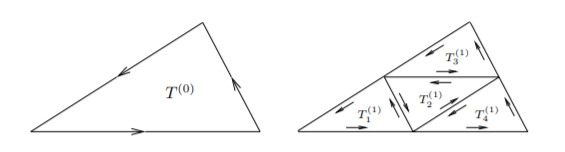
\includegraphics[height=8cm,width=16cm]{triangle.png} 
   \end{minipage}
\end{center}

Obviously, we may parametrize the boundaries of these triangles so that 
\begin{align*}
\int_{ \partial T^{(0)}}fdz= \sum_{n=1}^4 \int_{\partial T^{(1)}_n} fdz
\end{align*}
Taking absolute value on both side, we deduce 
\begin{align*}
  \abso{\int_{\partial  T^{(0)}}fdz }\leq 4 \abso{\int_{\partial  T^{(1)}_j}fdz}\text{ for some $j \in \set{1,2,3,4}$}
\end{align*}
Denote $T_j^{(1)}$ by $T^{(1)}$. Repeating this process, we obtain a decreasing sequence of triangles 
\begin{align*}
T^{(0)} \supseteq T^{(1)} \supseteq \cdots \supseteq T^{(n)} \supseteq \cdots 
\end{align*} 
with the property that
\begin{align}
\label{pe1}
\abso{\int_{\partial  T^{(0)}}fdz}\leq 4^n \abso{\int_{\partial T^{(n)}}fdz}
\end{align}
Let $d^{(n)}\text{ and }p^{(n)}$ denote the diameter and perimeter of $T^{(n)}$ for all $n\inz_0^+$. Some tedious effort shows that 
\begin{align}
\label{pe2}
d^{(n)}=2^{-n}d^{(0)}\text{ and }p^{(n)}=2^{-n}p^{(0)}
\end{align}
\myref{Theorem}{DSoC} implies 
\begin{align*}
\bigcap_{n\inn} T^{(n)}=\set{z_0}\text{ for some }z_0 \in D
\end{align*}
Because $f$ is holomorphic at  $z_0$, we may write $f:D\rightarrow \C$ by 
\begin{align*}
f(z)=f(z_0)+f'(z_0)(z-z_0)+o(z-z_0)(z-z_0)
\end{align*}
Clearly the first two terms have antiderivatives. Using \myref{Equation}{pe1} and \myref{Equation}{pe2}, we may now estimate 
\begin{align*}
 \abso{\int_{\partial T^{(0)}}f(z)dz}\leq  4^n\abso{\int_{\partial T^{(n)}} f(z)dz}&= 4^n\abso{\int_{\partial  T^{(n)}} o(z-z_0)(z-z_0)dz}\\
  &\leq 4^np^{(n)}d^{(n)}\max_{ z\in \partial T^{(n)}}\abso{o(z-z_0)}\\
  &= p^{(0)}d^{(0)} \max_{z \in \partial T^{(n)}} \abso{o(z-z_0)}\to 0\text{ as }n\to \infty
\end{align*}
\end{proof}
\begin{mdframed}
By $D\subseteq \C$ being \textbf{star-convex with center $z_*$}, we mean that for all $z \in D$, the contour $\gamma :[0,1]\rightarrow \C$ defined by 
\begin{align*}
\gamma (t)\triangleq z_*+t(z-z_*)
\end{align*}
satisfy $\gamma ([0,1])\subseteq D$. 
\end{mdframed}
\begin{theorem}
\textbf{(Existence of antiderivative on star-convex domain)} Suppose $D\subseteq \C$ is open and star-convex with centre  $z_*$. If $f:D\rightarrow \C$ is holomorphic, then $F:D\rightarrow \C$ defined by 
\begin{align*}
F(z)\triangleq \int_\gamma f(w)dw\text{ where }\gamma :[0,1]\rightarrow D\text{ is defined by }\gamma(t)\triangleq z_*+t(z-z_*)
\end{align*}
is an antiderivative of $f$. 
\end{theorem}
\begin{proof}
Fix $z_0 \in D$. Because $D$ is open, there exists some open ball $B_\epsilon (z_0)$ small enough to be contained by $D$. For all $z\in B_\epsilon (z_0)$, the closed triangle $T$ specified by the vertices $\set{z_*,z,z_0}$ is contained by $D$, since all $p\in  T$ lies in some line segment joining $z_*$ and $w$ where $w$ is some point that lies in the line segment joining $z$ and  $z_0$.  We then can apply \customref{CTft}{Cauchy's Integral Theorem for triangles} to have the estimate 
\begin{align*}
  \abso{\frac{F(z)-F(z_0)}{z-z_0}-f(z_0)}&= \abso{\frac{\int_\gamma [f(w)-f(z_0)]dw}{z-z_0}}\\
  &\leq \max_{w \in \gamma }\abso{f(w)-f(z_0)}\to 0\text{ as }z \to z_0
\end{align*}
where $\gamma$ is the line segment traveling from $z_0$ to  $z$.  
\end{proof}
\begin{mdframed}
At this point, it is appropriate for us to define \textbf{the winding number $w(\gamma ,z_0)$ of a contour $\gamma :[a,b]\rightarrow \C$ around some point $z_0\not\in \gamma $} by 
\begin{align*}
w(\gamma ,z_0)\triangleq  \frac{1}{2\pi  i}\int_{\gamma } \frac{1}{z-z_0}dz
\end{align*}
Immediately, we see that our definition satisfy our geometric intuition in the sense that the circle $\gamma :[0,2\pi  ]\rightarrow \C$ is defined by 
\begin{align*}
\gamma (t)\triangleq z_0 + e^{it}
\end{align*}
have winding number  
\begin{align*}
w(\gamma ,z_0)= \frac{1}{2\pi i}\int_0^{2\pi } e^{- it }ie^{it}dt= 1
\end{align*}
Moreover, we expect any closed contour $\gamma :[a,b]\rightarrow \C$ to have integer-valued winding number. This is true. Consider $f:[a,b]\rightarrow \C$ defined by 
\begin{align*}
f(t)\triangleq \frac{1}{2\pi  i}\int_a^t \frac{\gamma '(s)}{\gamma (s)-z_0}ds
\end{align*}
One may check by direct computation that 
\begin{align*}
\frac{d}{dt}e^{-2\pi  if (t)}(\gamma (t)-z_0)\equiv 0 
\end{align*}
It then follows from $\gamma $ being closed that 
\begin{align*}
e^{-2\pi  if(a)}=e^{-2\pi  if(b)}
\end{align*}
which implies 
\begin{align*}
w(\gamma ,z_0)=f(b)=f(a)+n=n\inz
\end{align*}
Given some contour $\gamma :[a,b]\rightarrow \C$, if we define $g:\C\setminus \gamma \rightarrow \C$ by 
\begin{align*}
g(z)\triangleq w(\gamma ,z)
\end{align*}
we see that $g$ is continuous, since if $z_0\not\in \gamma $, we may find $D_r(z_0)$ disjoint with $\gamma $ and obtain the estimate 
 \begin{align*}
\abso{w(\gamma ,z_0)-w(\gamma ,z_1)}&= \frac{1}{2\pi  }\abso{\int_\gamma \Big[ \frac{1}{z-z_0}-\frac{1}{z-z_1} \Big]dz} \\
&=\frac{1}{2\pi  }\abso{\int_{\gamma } \frac{z_1-z_0}{(z-z_0)(z-z_1)}dz} \\
&\leq \frac{L \abso{z_1-z_0}}{ r^2 \pi  }\text{ where }L\text{ is the length of }\gamma 
\end{align*}
as long as $\abso{z_0-z_1}<\frac{r}{2}$. The continuity of $g$ together with the fact that  $g$ can only be integer-valued implies that  $g$ is constant on any connected component of  $\C \setminus \gamma $. We may now finally state our version of \customref{CIT}{Cauchy Integral Theorem}. 
\end{mdframed}
\begin{theorem}
\label{CIT}
\textbf{(Cauchy Integral Theorem)} Suppose $D\subseteq \C$ is open and $f:D\rightarrow \C$ is holomorphic. If $\gamma :[a,b]\rightarrow \C$ is a closed contour lying in $D$ such that  $w(\gamma ,z)=0$ for all $z\not\in D$, then 
\begin{align*}
\int_\gamma  fdz=0 
\end{align*}
\end{theorem}
\begin{proof}
As Prof Frank remarked, the proof is omitted here for being too long and tricky. 
\end{proof}
\begin{theorem}
\label{CIF}
\textbf{(Cauchy Integral Formula)}  Let $U\subseteq \C$ be open, $D$ be an closed disk contained by  $U$, and $C$ be a closed contour running through the boundary of $D$ counterclockwise. If $f:U\rightarrow \C$ is holomorphic and $a\in D^\circ $, then 
\begin{align*}
f(a)= \frac{1}{2\pi  i}\int_C \frac{f(z)}{z-a}dz
\end{align*}
\end{theorem}
\begin{proof}
Fix $\epsilon $. Let $\delta$ satisfy 
\begin{align*}
\abso{z-a}\leq \delta \implies  \abso{f(z)-f(a)}\leq \epsilon 
\end{align*}
With a geometric argument using \customref{CIT}{Cauchy Integral Theorem}, one have 
\begin{align*}
\int_C \frac{f(z)}{z-a}dz=  \int_{\gamma  } \frac{f(z)}{z-a}dz
\end{align*}
where $\gamma :[0,2\pi ]\rightarrow D^\circ $ is defined by  
\begin{align*}
\gamma (t)\triangleq a+ \delta e^{it} 
\end{align*}
The proof then follows from the estimation 
\begin{align*}
  \abso{f(a)- \frac{1}{2\pi i}  \int_C \frac{f(z)}{z-a}dz}&= \abso{f(a)- \frac{1}{2\pi  i}\int_\gamma  \frac{f(z)}{z-a}dz} \\
                              &= \abso{f(a)- \frac{1}{2\pi  i}\int_0^{2\pi  } \frac{f(a+ \delta e^{it})}{\delta e^{it} } i\delta e^{i t} dt}  \\
                              &= \frac{1}{2\pi } \abso{\int_0^{2\pi  } f(a+ \delta e ^{it})- f(a)dt}\leq \epsilon 
\end{align*}
\end{proof}
\begin{theorem}
\label{Hfaa}
\textbf{(Holomorphic functions are analytic)} Let $U\subseteq \C$ be an open, $D$ be an closed disk contained by $U$ and centering $a$ with radius  $R$. Let $C$ be a closed contour running through the boundary of $D$ counterclockwise. If we define for all $n\geq 0$ 
\begin{align*}
c_n\triangleq  \frac{1}{2 \pi  i}\int_C \frac{f(z)}{(z-a)^{n+1}}dz
\end{align*}
then the power series 
\begin{align*}
  \sum_{n=0}^{\infty} c_n (z-a)^n
\end{align*}
agrees with $f$ on $D^{\circ }$. 
\end{theorem}
\begin{proof}
Let $z\in D^{\circ }$. By \customref{CIF}{Cauchy's Integral Formula}, we have 
\begin{align*}
f(z)&= \frac{1}{2\pi  i}\int_C \frac{f(w)}{w-z}dw \\
&=\frac{1}{2\pi  i}\int_C f(w)\Big[ \frac{1}{w-a} + \frac{z-a}{(w-a)^2}+ \cdots + \frac{(z-a)^m}{(w-a)^{m+1}} + \frac{(z-a)^{m+1}}{(w-a)^{m+1}(w-z)} \Big]dw \\
&=\sum_{n=0}^{m} c_n (z-a)^n + \frac{1}{2\pi  i}\int_C \frac{(z-a)^{m+1}}{(w-a)^{m+1}(w-z)}dw
\end{align*}
The proof then follows from noting  $\abso{\frac{z-a}{w-a}}<1$ and direct estimation of \myref{Equation}{LM}. 
\end{proof}
\begin{mdframed}
What follows from the fact  \customref{Hfaa}{holomorphic functions are analytic} and 
\customref{TT}{Taylor's Theorem for Power Series} is that if $f$ is holomorphic on some open disk  $D_{r+\epsilon }(a)$ and $C$ is the closed contour running through the boundary of  $D_r(a)$ counterclockwise, then we have a nice formula  
\begin{align*}
f^{(n)}(a)=  \frac{n!}{2\pi  i}\int_C \frac{f(z)}{(z-a)^{n+1}}dz
\end{align*}
which agrees with our \customref{CIF}{Cauchy integral Formula}.\\ 

In particular, we often encounter  complex function $f:\C\rightarrow \C$ that is \textbf{entire}, i.e., $f$ is holomorphic on the whole $\C$. \myref{Theorem}{Hfaa} states that for all $R>0$, if we let  $C$ be the closed contour running through the boundary of the open disk centering $0$ with radius  $R$  counterclockwise, then 
\begin{align*}
f=\sum_{n=0}^{\infty}c_{n,R} z^n \text{ on the open disk with radius }R
\end{align*}
for $c_{n,R}$ given in \myref{Theorem}{Hfaa}. Let $R_1< R_2$. Trivially, 
\begin{align*}
\sum_{n=0}^{\infty} c_{n,R_1}z^n=\sum_{n=0}^{\infty} c_{n,R_2}z^n\text{ on the open disk with radius }R_1
\end{align*}
It then follows from \customref{Identity Theorem}{Identity Theorem} that 
\begin{align*}
c_{n,R_1}=c_{n,R_2}\text{ for all }n
\end{align*}
Letting $R\to \infty$, we may now just write 
\begin{align*}
f(z)= \sum_{n=0}^{\infty}c_nz^n\text{ on }\C
\end{align*}
\end{mdframed}
\begin{theorem}
\label{LV}
\textbf{(Liouville's Theorem)} If entire $f:\C\rightarrow \C$ is bounded, then $f$ is constant. 
\end{theorem}
\begin{proof}
Write 
\begin{align*}
f(z)=\sum_{n=0}^{\infty}c_nz^n\text{ on }\C
\end{align*}
By \myref{Theorem}{Hfaa}, 
\begin{align*}
c_n= \frac{1}{2\pi i}\int_{C_r} \frac{f(z)}{z^{n+1}}dz
\end{align*}
where $C_r$ is the closed contour running through the boundary of the open disk centering  the origin with radius  $r$. Let $n\geq 1$, and let  $M$ be an upper bound of $\abso{f}$. The proof then following from letting $r \to \infty$ in the below estimation 
\begin{align*}
\abso{c_n}= \frac{1}{2\pi } \cdot (2\pi r) \cdot \max_{C_r} \abso{\frac{f(z)}{z^{n+1}}} \leq \frac{M}{r^n}
\end{align*}
\end{proof}
\section{Residue Formula}
\begin{abstract}

\end{abstract}
\begin{mdframed}
Before we begin developing this section, we first give the following remark. Let  
\begin{align*}
0<R_1 <r_1<r_2<R_2 < \infty
\end{align*}
Let $C_1,C_2$ respectively be closed contours running through the boundary of $D_{r_1}(0),D_{r_2}(0)$. If $f$ is holomorphic on on $R_1 < \abso{z}<R_2$, then 
\begin{align*}
\int_{C_1} f(z)dz= \int_{C_2}f(z)dz
\end{align*}
by a simple geometric argument. Therefore, we may give the next Theorem a well-defined statement. 
\end{mdframed}
\begin{theorem}
\label{LTC}
\textbf{(Laurent's Theorem)} Suppose
\begin{align*}
0\leq R_1 <r< R_2 \leq \infty
\end{align*}
$C_r$ is a closed contour running through the circle centering $z_0$ with radius $r$ counterclockwise, and $f$ is holomorphic on the annulus $R_1 < \abso{z-z_0} < R_2$. If we define 
\begin{align*}
c_n\triangleq  \frac{1}{2\pi  i} \int_{C_r} \frac{f(z)}{(z-z_0)^{n+1}}dz\text{ for all }n\inz
\end{align*}
Then $\sum_{n\geq 0} c_nh^n$ converge for $\abso{h}<R_2$, $\sum_{n<0} c_nh^{n}$ converge for $\abso{h}>R_1$ and 
\begin{align*}
f(z_0+h)= \sum_{n\inz} c_nh^n\text{ on the annulus }R_1 < \abso{h}< R_2
\end{align*}
\end{theorem}
\begin{proof}
Fix some  $h\inc$ such that $R_1 < \abso{h}<R_2$. Let $r_1,r_2$ satisfy 
 \begin{align*}
R_1 < r_1 < \abso{h}< r_2 < R_2
\end{align*}
And let $C_{r_1},C_{r_2}$ respectively be closed contours running through the circle centering $z_0$ with radius  $r_1,r_2$ counterclockwise. We first show that 
\begin{align*}
  \vi{f(z_0+h)= \frac{1}{2\pi  i}\int_{C_{r_1}} \frac{f(z)}{z-(z_0+h)}dz- \frac{1}{2\pi i}\int _{C_{r_2}} \frac{f(z)}{z-(z_0+h)}dz}
\end{align*}
\end{proof}
\begin{mdframed}
With \customref{LTC}{Laurent's Theorem}, given holomorphic $f:D_\epsilon (z_0)\setminus \set{z_0}\rightarrow \C$, we may write 
\begin{align*}
f(z)= \sum_{n\inz} c_n (z-z_0)^n\text{ for } 0<\abso{z-z_0}< \epsilon 
\end{align*}
If $c_n=0$ for all $n<0$, obviously we may define  $f(z_0)\triangleq c_0$, so that $f$ is still holomorphic after such extension. If this is the case, we say $f$ has a  \textbf{removable singularity at $z_0$}.     
\end{mdframed}
\begin{theorem}
\label{RoRS}
\textbf{(Riemann's removable singularity Theorem)} Given holomorphic $f:D_\epsilon (z_0)\setminus \set{z_0}\rightarrow \C$ 
\begin{align*}
z_0\text{ is a removable singularity of $f$ }\iff f\text{ is bounded on some }D_\delta (z_0)\setminus \set{z_0}
\end{align*}
\end{theorem}
\begin{proof}
From left to right is clear. Suppose $f$ is bounded by $M$ on $D_\delta(z_0)\setminus \set{z_0}$. Because 
\begin{align*}
c_n=\frac{1}{2\pi  i}\int_{C_r}f(z)(z-z_0)^{-n-1}dz
\end{align*}
We may estimate 
\begin{align*}
  \abso{c_n}\leq \frac{1}{2\pi }(2\pi r )( M r^{-n-1})= Mr^{-n}
\end{align*}
The proof then follows from letting $n<0$ and $r \to 0$. 
\end{proof}
\begin{mdframed}
If for some $m<0$, we have  
 \begin{align*}
c_m \neq 0\text{ and }c_n=0\text{ for all }n\leq m
\end{align*}
then we say $f$ has a  \textbf{pole of order $m$ at  $z_0$}. If a pole is of order $1$, we say such pole is a  \textbf{simple pole}.  
\end{mdframed}
\begin{theorem}
\textbf{(Recognition of Pole)} Given holomorphic $f:D_\epsilon (z_0)\setminus \set{z_0}\rightarrow \C$ 
\begin{align*}
f\text{ has a pole of order }m\text{ at }z_0\iff \lim_{z\to z_0}(z-z_0)^mf(z)\inc^*
\end{align*}
\end{theorem}
\begin{proof}
From left to right is clear. From right to left, define $g:D_\epsilon (z_0)\setminus \set{z_0}\rightarrow \C$ by 
\begin{align*}
g(z)\triangleq (z-z_0)^m f(z)
\end{align*}
From premise, we may deduce $g$ is bounded on some  $D_\delta(z_0)\setminus \set{z_0}$. Therefore, by \myref{Theorem}{RoRS}, $g$ has a removable singularity at $z_0$. Thus, we may write 
 \begin{align*}
g(z)=\sum_{n=0}^{\infty}a_n z^n
\end{align*}
where $a_0\neq 0$ by premise. The proof then follows from writing $f$ in terms of $a_n$.  
\end{proof}
\begin{mdframed}
Writing holomorphic $f:D_\epsilon (z_0)\setminus \set{z_0}\rightarrow \C$ in terms of Laurent Series  
\begin{align*}
f(z)= \sum_{n\inz} c_n (z-z_0)^n 
\end{align*}
We define the \textbf{residue of $f$ at  $z_0$} to be 
\begin{align*}
\operatorname{Res}(f,z_0)\triangleq c_{-1}
\end{align*}
If there are infinitely many $n<0$ such that $c_n\neq 0$, we say $f$ has a \textbf{essential singularity} at $z_0$. Obviously, if  $f$ has a removable singularity at  $z_0$, then the residue of  $f$ at $z_0$ is  $0$. Immediately, from direct computation with Laurent expansion of $f:D_\epsilon (z_0)\setminus \set{z_0}\rightarrow \C$, we may conclude the following easy ways to compute residue for relatively simple function. 
\end{mdframed}
\begin{theorem}
\textbf{(Calculation of Residue)} If holomorphic $p,q:D_\epsilon (z_0)\rightarrow \C$ satisfies 
\begin{align*}
p(z_0)\neq 0\text{ and }q(z_0)=0,q'(z_0)\neq 0 
\end{align*}
Then $f=\frac{p}{q}$ has a simple pole at $z_0$ and 
 \begin{align*}
\operatorname{Res}(f,z_0)= \frac{p(z_0)}{q'(z_0)}
\end{align*}
If $f:D_\epsilon (z_0)\setminus \set{z_0}\rightarrow \C$ has a pole of order $m$ at  $z_0$,  then 
 \begin{align*}
\operatorname{Res}(f,z_0)=  \lim_{z\to z_0} \frac{1}{(m-1)!} \Big( \frac{d}{dz} \Big)^{m-1} (z-z_0)^m f(z)
\end{align*}
\end{theorem}
\begin{theorem}
\label{CRT}
\textbf{(Cauchy's Residue Theorem)} Suppose that $f$ is holomorphic in an open set containing a positively oriented  Jordan curve $\gamma $ and its interior, except for poles at the points $z_1,\dots ,z_N$ inside $\gamma $. Then 
\begin{align*}
\int_{\gamma }f(z)dz = 2\pi  i\sum_{n=1}^N \operatorname{Res} (f,z_n)
\end{align*}
\end{theorem}
\begin{mdframed}
  Using \customref{CRT}{the residue theorem}, we may compute the following integral that will definitely exists in context of Fourier analysis.   
\end{mdframed}
\begin{Example}{\textbf{(Poisson Kernel)}}{}
\begin{align*}
  \int_0^{\pi } \frac{\log x}{1+x^2}dx
\end{align*}
\end{Example}
\begin{mdframed}
Let $D \subseteq \C$ be open connected, $f:D\rightarrow \C$ be holomorphic. Suppose $f$ does not vanish identically on  $D$.  \customref{Identity Theorem}{Identity Theorem} tell us that the set of \textbf{zeros}
\begin{align*}
Z\triangleq \set{z\in D: f(z)=0}
\end{align*}
must have no limit point in $D$. Therefore, for each zero $z_0 \in Z$, when we write locally 
\begin{align*}
  f(z)= \sum_{n=0}^{\infty} c_n(z-z_0)^n
\end{align*}
there exists some smallest $n\geq 1$ such that $c_n \neq 0$. We then say $f$ has a  \textbf{zero of order $n$ at $z_0$}, and if  $n=1$, we say this zero is  \textbf{simple}. \\

Let $z_0\inc$. Given some holomorphic $f:D_\epsilon (z_0)\setminus \set{z_0}\rightarrow \C$, we say $f$ has a \textbf{removable singularity at $z_0$} if we may define $f(z_0)$ to be some complex number so that $f:D_\epsilon (z_0)\rightarrow \C$ is holomorphic. Suppose $f:D_\epsilon (z_0)\setminus \set{z_0}\rightarrow \C^*$. We say $f$ has a  \textbf{pole of order $n$ at $z_0$} if the function $g:D_\epsilon (z_0)\rightarrow \C$ defined by 
\begin{align*}
g(z)\triangleq \begin{cases}
  \frac{1}{f(z)}& \text{ if $z\neq z_0$ }\\
  0& \text{ if $z=z_0$ }
\end{cases}
\end{align*}
is holomorphic with the order $n$ at zero  $z_0$. Obviously, there exists an unique holomorphic $h:D_\epsilon (z_0)\rightarrow \C$ such that 
\begin{align*}
g(z)= (z-z_0)^n h(z)
\end{align*}
It is clear that $h$ does not vanish on  $D_\epsilon (z_0)$. Therefore, we may write 
\begin{align*}
G(z)= \frac{1}{h(z)}
\end{align*}
so that $G:D_\epsilon (z_0)\rightarrow \C$ is holomorphic and write 
\begin{align*}
f(z)= \frac{G(z)}{(z-z_0)^n}=\sum_{k=-n}^{\infty}a_k (z-z_0)^k
\end{align*}
We then call 
\begin{align*}
\sum_{k=-n}^{-1}a_k(z-z_0)^k
\end{align*}
the \textbf{principal part of $f$ at the pole $z_0$} and 
\begin{align*}
\operatorname{Res}_{z_0}f\triangleq a_{-1}
\end{align*}
the \textbf{residue of $f$ at the pole  $z_0$}. It is clear from the Laurent expansion of $f$ and direct computation that   
\begin{align*}
\operatorname{Res}_{z_0}f=
\end{align*}
\end{mdframed}
\section{Script}
\begin{question}{}{}
There are three types of isolated singularities: removable singularity, poles and essential singularity. Provide the definition of each type and give an example.  
\end{question}
\begin{proof}
Let $f:D_\epsilon (z_0)\setminus \set{z_0}\rightarrow \C$ be holomorphic so that $f$ has an isolated singularity at  $z_0$. By Laurent's Theorem, we may express $f$ as a Laurent series 
\begin{align*}
f(z)= \sum_{n=-\infty}^{\infty} c_n(z-z_0)^n
\end{align*}
If $c_n=0$ for all negative $n$, say 
\begin{align*}
f(z)= (z-z_0)^2 + 7 \text{ on }D_\epsilon (z_0)\setminus \set{z_0}
\end{align*}
we say $f$ has a removable singularity at $z_0$. If there are only finite numbers of negative $n$ such that $c_n\neq 0$, and $m$ is the smallest integer such that
\begin{align*}
c_n \neq 0 \text{ for }n=m
\end{align*}
we say $f$ has a pole of order $m$ at $z_0$. For example, $f$ can be 
 \begin{align*}
f(z)=\frac{1}{z-z_0}\text{ on }D_\epsilon (z_0)\setminus \set{z_0}
\end{align*}
If there are infinite number of negative $n$ such that  $c_n \neq 0$, for example, 
\begin{align*}
f(z)= e^{\frac{1}{(z-z_0)}}= \sum_{n=0}^{\infty} \frac{1}{n!}(z-z_0)^{-n}\text{ on }D_\epsilon (z_0)\setminus \set{z_0}
\end{align*}
we say $f$ has an essential singularity at $z_0$. 
\end{proof}
\begin{question}{}{}
State the definition of the residue of a function at an isolated singularity. 
\end{question}
\begin{proof}
Let $f:D_\epsilon (z_0)\setminus \set{z_0}\rightarrow \C$ be holomorphic so that $f$ has an isolated singularity at  $z_0$. By Laurent's Theorem, we may express $f$ as a Laurent series 
\begin{align*}
f(z)= \sum_{n=-\infty}^{\infty} c_n(z-z_0)^n
\end{align*}
The residue of $f$ at  $z_0$ is defined to be $c_{-1}$. 
\begin{align*}
\operatorname{Res}(f,z_0)\triangleq c_{-1}
\end{align*}
\end{proof}
\begin{question}{}{}
If $z_0$ is a simple pole of  $f$, prove that 
\begin{align*}
\operatorname{Res}(f,z_0)= \lim_{z\to z_0} (z-z_0)f(z)
\end{align*}
\end{question}
\begin{proof}
Because $z_0$ is a simple pole of  $f$, we may write 
 \begin{align*}
   f(z)= [\operatorname{Res}(f,z_0)](z-z_0)^{-1}+ \sum_{n=0}^{\infty} c_n(z-z_0)^n
\end{align*}
This give us 
\begin{align*}
\lim_{z\to z_0}(z-z_0)f(z)&= \lim_{z\to z_0}\operatorname{Res}(f,z_0)+ \sum_{n=0}^{\infty}c_n(z-z_0)^{n+1} \\
&=\operatorname{Res}(f,z_0)+ \sum_{n=0}^{\infty} \lim_{z\to z_0}c_n (z-z_0)^{n+1} \\
&=\operatorname{Res}(f,z_0)
\end{align*}
\end{proof}
\begin{question}{}{}
If  $f(z)=\frac{q(z)}{p(z)}$ where $p$ and $q$ are holomorphic, and  $z_0$ is a simple zero of  $p$, prove that 
\begin{align*}
\operatorname{Res}(f,z_0)= \frac{q(z_0)}{p'(z_0)}
\end{align*}
\end{question}
\begin{proof}
Because $z_0$ is a simple zero of $p$, we know 
\begin{align*}
p'(z_0)\neq 0
\end{align*}
If $q(z_0)\neq 0$, then $f$ has a simple pole at $z_0$, and from result of last question we may compute 
 \begin{align*}
\operatorname{Res}(f,z_0)&= \lim_{z\to z_0} \frac{(z-z_0)q(z)}{p(z)-p(z_0)}= \frac{q(z_0)}{p'(z_0)} 
\end{align*}
\end{proof}
\begin{question}{}{}
If $z_0$ is a pole of  $f$ of order $m$, prove that 
 \begin{align*}
\operatorname{Res}(f,z_0)=\lim_{z\to z_0} \frac{1}{(m-1)!}\Big(\frac{d}{dz}\Big)^{m-1} g(z)
\end{align*}
where $g(z)=(z-z_0)^m f(z)$
\end{question}
\begin{proof}
Because $z_0$ is a pole of $f$ of order $m$, we may write 
 \begin{align*}
f(z)=\sum_{n=-m}^\infty c_n (z-z_0)^n\text{ and }g(z)=\sum_{n=0}^{\infty} c_{n-m}(z-z_0)^n
\end{align*}
Or write 
\begin{align*}
  g(z)= c_{-m}+c_{-m+1} (z-z_0)   + \cdots + c_{-1}(z-z_0)^{m-1} + c_0(z-z_0)^m +\cdots 
\end{align*}
Compute 
\begin{align*}
g^{(m-1)}(z)= \frac{(m-1)!}{0!}c_{-1}+\frac{m!}{1!}c_0(z-z_0)+ \frac{(m+1)!}{2!}c_1(z-z_0)^2 + \cdots  
\end{align*}
This give us 
\begin{align*}
\lim_{z\to z_0} \frac{1}{(m-1)!}g^{(m-1)}(z)= c_{-1}= \operatorname{Res}(f,z_0)
\end{align*}
\end{proof}
\begin{question}{}{}
Find the residue of the following function at the indicated points: 
\begin{enumerate}[label=(\alph*)]
  \item $\frac{z}{(2-3z)(4z+3)}$ at $z= \frac{2}{3}$. 
  \item $\frac{z-\frac{1}{6}z^3 - \sin z}{z^8}$ at $z=0$. 
\end{enumerate}
\end{question}
\begin{proof}
For the first function, observe  
\begin{align*}
\lim_{z\to \frac{2}{3}} (z- \frac{2}{3}) \cdot \frac{z}{(2-3z)(4z+3)}= \lim_{z\to \frac{2}{3}}\frac{z}{-3(4z+3)}= \frac{2}{-51}\neq 0
\end{align*}
which implies $z=\frac{2}{3}$ is a simple pole. Therefore, from the question earlier, we may deduce its residue is exactly $\frac{2}{-51}$. For the second function, we can just compute its Laurent series by 
\begin{align*}
\frac{z- \frac{1}{6}z^3- \sin z}{z^8}&= \frac{1}{z^7}- \frac{1}{6z^5} - \frac{1}{z^8}\sum_{n=0}^{\infty}  \frac{(-1)^n}{(2n+1)!}z^{2n+1} \\
&=\frac{1}{5!}z^{-3}+ \frac{-1}{7!}z^{-1}+ \frac{1}{9!}z + \cdots 
\end{align*}
Therefore, its residue is $\frac{-1}{7!}$. 
\end{proof}
\begin{question}{}{}
Evaluate 
\begin{align*}
\int_{-\pi }^{\pi } \frac{d\theta}{5+ 3 \cos \theta}
\end{align*}
\end{question}
\begin{proof}
Define $\gamma :[-\pi ,\pi ]\rightarrow \C$ by 
\begin{align*}
\gamma (t)=e^{it}
\end{align*}
We have 
\begin{align*}
I\triangleq -2i\int _{\gamma } \frac{dz}{3z^2+10z+3}&= \int_\gamma  \frac{dz}{\frac{3i}{2}z^2 + 5iz+ \frac{3}{2}i} \\
&=\int_{\gamma } \frac{1}{5+ \frac{3}{2}(z+ \frac{1}{z})} \cdot \frac{1}{iz} dz\\
&=\int_{-\pi }^{\pi } \frac{1}{5+ \frac{3}{2}(e^{it}+e^{-it})} \cdot \frac{ie^{ it}}{i e^{it}}dt \\
&=\int_{-\pi }^{\pi } \frac{1}{5+ 3 \cos t}dt
\end{align*}
In summary 
\begin{align*}
\int_{-\pi }^{\pi } \frac{d\theta}{5+ 3 \cos \theta}&= -2i \int_{\gamma } \frac{dz}{3z^2+10z+3} 
\end{align*}
Note that 
\begin{align*}
\frac{1}{3z^2+10+3}= \frac{1}{(3z+1)(z+3)}
\end{align*}
have two simple poles $z=-3$ and  $z= \frac{1}{-3}$, and have residue $\frac{1}{8}$ at pole $z=\frac{1}{-3}$. It then follows from residue theorem that 
\begin{align*}
\int_{-\pi }^{\pi } \frac{d\theta}{5+ 3 \cos \theta}= - 2i \cdot 2\pi  i \cdot \frac{1}{8}= \frac{\pi }{2} 
\end{align*}
\end{proof}
\begin{question}{}{}
Evaluate 
\begin{align*}
\int^{\infty}_{- \infty } \frac{dx}{x^2+2x+2}
\end{align*}
\end{question}
\begin{proof}
Let $S_R:[0 ,\pi ]\rightarrow \C$ be the semi-circle $S_R(t)\triangleq Re^{it}$, $L_R:[-R,R]\rightarrow \C$ be the line segment $L_R(t)\triangleq t$, and $\gamma$ the wedge $\gamma =S_R+L_R$. By residue theorem, 
\begin{align*}
\int_{\gamma } \frac{dz}{z^2+2z+2}= 2\pi i \cdot \frac{1}{2i}=\pi 
\end{align*}
for large enough $R$. Observe 
\begin{align*}
  \abso{\int_{S_R} \frac{dz}{z^2+2z+2} }\leq \pi R \cdot \max_{S_R} \frac{1}{\abso{z+1-i}\cdot \abso{z+1+i}} \leq  \frac{\pi  R}{(R- \sqrt{2} )^2} 
\end{align*}
This implies 
\begin{align*}
\lim_{R\to \infty} \int_{S_R} \frac{dz}{z^2+2z+2}= 0
\end{align*}
Therefore, 
\begin{align*}
\int_{-\infty}^{\infty} \frac{dx}{x^2+2x+2}&= \lim_{R\to \infty}\int_{L_R} \frac{dz}{z^2+2z+2} \\
&=\lim_{R\to \infty} \pi  - \int_{S_R} \frac{dz}{z^2+2z+2}=\pi 
\end{align*}
\end{proof}
\begin{question}{}{}
Evaluate 
\begin{align*}
\int_{-\infty}^{\infty} \frac{dx}{x^4+2x^2+1}
\end{align*}
\end{question}
\begin{proof}
Let $S_R:[0 ,\pi ]\rightarrow \C$ be the semi-circle $S_R(t)\triangleq Re^{it}$, $L_R:[-R,R]\rightarrow \C$ be the line segment $L_R(t)\triangleq t$, and $\gamma$ the wedge $\gamma =S_R+L_R$. By residue theorem, 
\begin{align*}
\int_{\gamma } \frac{dz}{z^4+2z^2+1}= 2\pi  i \lim_{z\to i} \frac{d}{dz} \frac{1}{(z+i)^2}= \frac{\pi }{2}
\end{align*}
for large enough $R$. Observe 
 \begin{align*}
\abso{\int_{S_R} \frac{dz}{z^4+2z^2+1}}\leq \pi  R \cdot \max_{S_R} \frac{1}{\abso{z+i}^2 \cdot \abso{z-i}^2}\leq \frac{\pi  R}{(R-1)^4}
\end{align*}
This implies 
\begin{align*}
\lim_{R\to \infty} \int_{S_R} \frac{dz}{z^4+2z^2+1} = 0
\end{align*}
Therefore, 
\begin{align*}
\int_{-\infty}^{\infty} \frac{dx}{x^4+ 2x^2+1}&= \lim_{R\to \infty} \int_{L_R} \frac{dz}{z^4+2z^2+1} \\
&=\lim_{R\to \infty} \frac{\pi }{2}- \int_{S_R} \frac{dz}{z^4+2z^2+1}= \frac{\pi }{2}
\end{align*}
\end{proof}
\end{document}
